\PassOptionsToPackage{demo}{graphicx}
\documentclass[authoryear, review, 12pt, draft]{elsarticle}
\usepackage{amssymb}
\usepackage{amsmath}
\usepackage{amsthm}
\usepackage{psfrag}
\usepackage{comment}
\usepackage[colorlinks]{hyperref}
%\usepackage{cleveref}
\usepackage{mathtools}
\usepackage{makecell}
\mathtoolsset{showonlyrefs=true}
\usepackage{alltt}
\usepackage{booktabs}
\usepackage{longtable}
\usepackage{threeparttablex}
\allowdisplaybreaks
%\modulolinenumbers[5]
\makeatletter
\def\ps@pprintTitle{%
	\let\@oddhead\@empty
	\let\@evenhead\@empty
	\def\@oddfoot{\reset@font\hfil\thepage\hfil}
	\let\@evenfoot\@oddfoot
}
\makeatother
\newcommand{\ra}[1]{\renewcommand{\arraystretch}{#1}}
%\usepackage{amssymb}
\graphicspath{ 
	{"C:/Users/msilva913/Documents/GitHub/Sunk_entry_costs_endogenous_variety_unemployment"}
	{"C:/Users/msilva913/Documents/GitHub/Sunk_entry_costs_endogenous_variety_unemployment/Programs baseline"}
	{"C:/Users/msilv/Documents/Github/Sunk-entry-costs--endogenous-variety--and-unemployment"}
	{"C:/Users/msilv/Documents/GitHub/Sunk-entry-costs--endogenous-variety--and-unemployment/Programs baseline"}
	{"C:/Users/msilv/Dropbox/Documents - Copy/Research/Sunk vacancy costs endogenous product variety labor market frictions/Draft/figs"}
	{"C:/Users/msilva913/Dropbox/Documents - Copy/Research/Sunk vacancy costs endogenous product variety labor market frictions/Draft/figs"}
	{"C:/Users/msilv/Dropbox/Documents - Copy/Research/Sunk vacancy costs endogenous product variety labor market frictions/Draft/figs"}
	{"C:/Users/msilv/Documents/GitHub/Sunk-entry-costs--endogenous-variety--and-unemployment/Data/Bartek analysis/data/results"}
}
\usepackage{tabularx}
\usepackage{comment}
\usepackage{subfig}
\usepackage[demo]{graphicx}
%\journal{Journal of Monetary Economics}
%\usepackage{amssymb}
%\usepackage{amsfonts}
\usepackage{geometry}
\usepackage{diagbox}
\usepackage{epstopdf}
\geometry{verbose,tmargin=2cm,bmargin=2cm,lmargin=2.25cm,rmargin=2.25cm} 
\newtheorem{theorem}{Theorem}
\newtheorem{proposition}{Proposition}
\newtheorem{lemma}{Lemma}
\newtheorem{corollary}{Corollary}
\newtheorem{example}{Example}
\newtheorem{remark}{Remark}
\newtheorem{definition}{Definition}
\usepackage{cite}
\usepackage{float}
\newcommand{\bi}{\begin{itemize}}
	\newcommand{\ei}{\end{itemize}}
\newcommand{\pfrac}[2]{\left(\dfrac{#1}{#2}\right)}
\newcommand{\ov}{\overline}
\newcommand{\deriv}[2]{\dfrac{\partial #1}{\partial #2}}
\newcommand{\der}[2]{\frac{\partial #1}{\partial #2}}
\renewcommand{\pfrac}[2]{\left(\frac{#1}{#2}\right)}
\newcommand{\bfrac}[2]{\left[\dfrac{#1}{#2}\right]}
\newcommand{\lfrac}[1]{\frac{#1}{#1-1}}
\newcommand{\curlyfrac}[2]{\left\{\frac{#1}{#2}\right\}}

% Double space footnotes
\newcommand{\note}[1]{\footnote{\begin{doublespace}#1\end{doublespace}}}
% Simplify ll notation
\newcommand{\ptil}{\tilde{p}}
\newcommand{\wtil}{\tilde{w}}
\newcommand{\Ctil}{\tilde{C}}
\newcommand{\Ntil}{\tilde{N}}
\newcommand{\Ltil}{\tilde{L}}
\newcommand{\Stil}{\tilde{S}}
\newcommand{\thetatil}{\tilde{\theta}}
\newcommand{\Ztil}{\tilde{Z}}
\newcommand{\rtil}{\tilde{r}}
\newcommand{\dtil}{\tilde{d}}
\newcommand{\Qtil}{\tilde{Q}}
\newcommand{\mutil}{\tilde{\mu}}
\usepackage{tikz}
\usetikzlibrary{shapes.geometric, arrows, shapes.multipart}
\tikzstyle{arrow} = [very thick, ->, >=stealth, blue!50]
\tikzstyle{startstop} = [ellipse, minimum width=3.5cm, minimum height=1.5cm, text centered, draw=magenta!50, fill=cyan!30]
\usetikzlibrary{arrows}
\definecolor{turquoise}{RGB}{64, 224, 208}

\begin{document}
	\begin{frontmatter}
		\begin{abstract}
			How do business formation and exit dynamics influence job creation and destruction? We develop a unified model of endogenous business formation and exit and labor market frictions and study its implications for unemployment and vacancy dynamics. Monopolistically competitive producers use labor and face exit risk from product obsolescence and stochastic fixed costs. Creating businesses and vacancies both require sunk costs, making them partially predetermined: if a product line survives, unfilled vacancies are reposted. We estimate the model via Bayesian simulated method of moments using aggregate technology, product destruction, and match separation shocks. When a firm exits, it immediately eliminates jobs and posted vacancies and reduces product variety, so vacancy persistence closely tracks product-line longevity. By contrast, match separation shocks destroy only filled jobs, generating counterfactual positive comovement of unemployment and vacancies. The loss of variety also dampens job creation and employment via an aggregate demand externality. Adverse technology shocks induce exit among high-cost firms, amplifying labor-market effects. Quantitatively, the model matches the volatility, autocorrelation, and cross-correlation of unemployment, vacancies, business formation, employment-to-unemployment transitions, and establishment exit, with technology and destruction shocks playing the predominant roles.
		\end{abstract}
		%\begin{keyword}
		%	labor market frictions \sep sunk entry costs \sep estimation \\
		%	\smallskip
		%	\text{JEL Classification: D10; E21; E22; E32; E37}\\
		%\end{keyword}
		
		\title{Role of business formation and exit for unemployment and vacancy dynamics}
		\author[affil1]{Mario Rafael Silva}
		\ead{msilva913@hkbu.edu}
		\author[affil2]{Marshall Urias}
		\address[affil1]{Department of Accountancy, Economics, and Finance, Hong Kong Baptist University}
		\ead{murias@phbs.pku.edu.cn}
		\address[affil2]{Peking University HSBC Business School}
		\author[affil3]{Zhesheng Qiu}
		\address[affil3]{Hong Kong University of Science and Technology}
		\ead{zheshqiu@ust.hk}
		\fntext[]{}
	\end{frontmatter}
	\section{Introduction}\label{sec:introduction}
	
	Labor market variables do not recover at equal speed, and the 
	disparity does not just depend on the severity of the initial shock. 
	The 2020 recession produced the highest peak unemployment rate of 
	any postwar episode --- 13.0 percent --- yet labor markets had 
	recovered within two years, accumulating only 26.6 percentage-point 
	quarters of total unemployment excess over twenty quarters from 
	recession onset. The 2008--09 recession generated a smaller peak unemployment rate of 9.9 percent yet produced 76.6 percentage-point 
	quarters of cumulative damage and a recovery stretching across six 
	years. The standard Diamond--Mortensen--Pissarides (DMP) framework, 
	in which all separations are identical and firms repost vacancies 
	freely after any job loss, offers no structural account of why two 
	recessions of comparable peak unemployment can generate such 
	different cumulative damage: the composition of job loss --- not 
	just its volume --- has no influence on persistence. We argue that a 
	key missing margin is firm destruction --- the permanent elimination 
	of business opportunities and their associated vacancy slots --- 
	which ran at 7.8 percent of base employment in 2008--09 but only 
	2.9 percent in 2020.\footnote{Financial frictions, nominal 
		rigidities, and other margins absent from the benchmark model have 
		each received substantial attention in the literature; we focus on 
		firm destruction and its interaction with endogenous business 
		formation.} When a firm exits, its vacancies vanish permanently and 
	must be rebuilt from scratch at sunk cost; recovery requires not 
	merely a rebound in profitability but a costly reconstruction of the 
	vacancy stock, generating a persistent outward shift of the 
	Beveridge curve. Provided vacancy continuation is sufficiently cheap  relative to initial creation, surviving firms repost after separation, so the aggregate vacancy stock partially self-corrects even while unemployment remains elevated, producing a transitory displacement along the Beveridge curve rather than a persistent  outward shift.
	
	\citet{coles_2018} show that extending the DMP model with finitely 
	elastic vacancy creation enables separation shocks to generate a 
	downward-sloping Beveridge curve and, jointly with technology shocks, 
	fit a broad set of labor market moments well. But CK assume a single 
	separation shock, conflating firm destruction and match dissolution 
	into one margin. \citet{gabrovski_2025} build on CK by distinguishing 
	between destruction of a product line $\delta$ and breakdown of a 
	match $s$, and show that under technology shocks alone, for 
	empirically relevant values of $\delta$, the model generates mild 
	unemployment--labor productivity comovement and matches other key 
	labor market moments, including the Beveridge curve. In both 
	frameworks, sunk entry costs make the vacancy stock predetermined: 
	$v_{t-1}$ enters the equilibrium alongside $u_t$, and surviving 
	firms repost vacancies freely following match dissolution, 
	substantially weakening the link between unemployment and 
	contemporaneous productivity.
	
	This paper opens additional channels related to business formation 
	and exit. First, we introduce love-of-variety preferences over 
	differentiated product lines, so that the number of active product 
	lines $N_t$ becomes a third independent state variable: greater 
	product diversity raises the return to posting vacancies, while 
	greater employment raises the resources available for product-line 
	formation. We segment the product and labor markets so that 
	producers can employ a mass of workers, avoiding any mechanical link 
	between employment and the range of product lines: $u_t$, $v_{t-1}$, 
	and $N_t$ are jointly determined in equilibrium without an accounting 
	restriction. Second, we endogenize firm exit, so that $\delta_t$ 
	responds to aggregate productivity and separation conditions: a 
	recession that reduces profitability or raises separation rates 
	induces higher exit, further depleting the vacancy stock and product variety and further suppressing job creation. Together these 
	extensions sharpen the asymmetry between $\delta$ and $s$ shocks: a firm-destruction shock simultaneously damages all three state variables --- raising $u_t$, depleting $v_{t-1}$, and eliminating product lines that would otherwise sustain vacancy creation 
	incentives --- while a match-separation shock raises $u_t$ but does not directly affect $v_{t-1}$ or $N_t$. We argue quantitatively that this three-channel amplification helps account for the cross-recession gap in cumulative labor market damage, and we identify the key 
	structural parameters using Bayesian simulated method of moments on unconditional moments, extended with Bayesian impulse response 
	matching to an externally identified firm-destruction shock.
	
	% Empirical motivation
	Three empirical facts motivate treating firm destruction as a 
	distinct and quantitatively important margin. \textit{First, establishment closings and openings constitute a large and cyclically sensitive component of gross job flows}. Table~\ref{tab:jf_t2_ext_2024} extends Table 2 in \citet{jaimovich_2008} through 2024Q4 using Business Economics Database (BED) data. Columns 1--2 of Table~\ref{tab:jf_t2_ext_2024} report the average fraction of quarterly gross job gains (losses) accounted for by opening (closing) establishments. Columns 3 and 4 report the ratio of the cyclical standard deviation of entry/exit flows to that of total flows, using the Hamilton (2018) regression filter ($h=8, p=4$) applied to raw levels. Columns 5 and 6 repeat the calculation with the HP filter ($\lambda=1600$), which closely reproduces \citet{jaimovich_2008}'s benchmark of approximately 0.33 in the original 1992--2006 sample.
	
	Columns 1 and 2 show that closing establishments account for 19.3 percent of gross job losses on average across all private-sector supersectors 
	--- a share that is remarkably stable across industries ranging from construction (20.5 percent) to financial activities (24.6 percent). The relative standard deviation columns show that closing-establishment 
	flows are meaningfully cyclical under both Hamilton and HP filters, with the total-private closing share moving at 0.152 times the 
	cyclical variation of unemployment under the Hamilton filter. 
	Translating these shares into rates, the quarterly establishment 
	exit rate averages 0.93 percent of base employment against a total 
	quarterly separation rate of 9.3 percent: most separations are 
	therefore not firm exits, which makes the $\delta$-vs-$s$ 
	decomposition empirically tractable --- the two margins are 
	separately measurable yet distinct enough that conflating them 
	materially distorts model predictions.
	%%%%%%%%%%%%%%%%
	\begin{table}[H]
		\centering
		\small
		\begin{tabular}{lcccccc}
			\toprule
			& \multicolumn{2}{c}{Mean share} & \multicolumn{2}{c}{Rel.\ std dev (Ham)} & \multicolumn{2}{c}{Rel.\ std dev (HP)} \\
			\cmidrule(lr){2-3}\cmidrule(lr){4-5}\cmidrule(lr){6-7}
			Industry & $\bar{g}^O$ & $\bar{g}^C$ & $\sigma^O/\sigma$ & $\sigma^C/\sigma$ & $\sigma^O/\sigma$ & $\sigma^C/\sigma$ \\
			\midrule
			\midrule
			\textbf{Total private} & 0.199 & 0.193 & 0.227 & 0.152 & 0.206 & 0.132 \\
			Natural resources \& mining & 0.163 & 0.156 & 0.281 & 0.177 & 0.261 & 0.176 \\
			Construction & 0.208 & 0.205 & 0.188 & 0.185 & 0.209 & 0.165 \\
			Manufacturing & 0.123 & 0.137 & 0.214 & 0.109 & 0.219 & 0.093 \\
			Wholesale trade & 0.203 & 0.226 & 0.251 & 0.184 & 0.260 & 0.143 \\
			Retail trade & 0.169 & 0.152 & 0.202 & 0.142 & 0.210 & 0.124 \\
			Transportation \& utilities & 0.163 & 0.169 & 0.236 & 0.118 & 0.194 & 0.097 \\
			Information & 0.206 & 0.209 & 0.284 & 0.310 & 0.301 & 0.269 \\
			Financial activities & 0.235 & 0.246 & 0.343 & 0.323 & 0.416 & 0.305 \\
			Prof.~\& business services & 0.205 & 0.211 & 0.242 & 0.156 & 0.236 & 0.133 \\
			Education \& health services & 0.203 & 0.211 & 0.307 & 0.151 & 0.246 & 0.125 \\
			Leisure \& hospitality & 0.241 & 0.196 & 0.173 & 0.168 & 0.174 & 0.158 \\
			Other services & 0.225 & 0.223 & 0.427 & 0.286 & 0.415 & 0.270 \\
			\midrule
			\multicolumn{7}{p{0.92\linewidth}}{\footnotesize \textit{Notes.} $\bar{g}^O$ ($\bar{g}^C$): mean share of gross job gains (losses) from opening (closing) establishments, $\sum G_O/\sum G$. Cols 3--4: relative std dev $\sigma^O/\sigma$ ($\sigma^C/\sigma$) via Hamilton (2018) filter ($h{=}8$, $p{=}4$), raw levels; robust to GFC/Covid outliers. Cols 5--6: same statistic via HP filter ($\lambda{=}1600$).} \\
			\bottomrule
		\end{tabular}
		\caption{Job Gains and Losses from Opening and Closing Establishments (\emph{Extended to 2024Q4 (BED end)}) \\[2pt]
			{\small\itshape Source: BLS Business Employment Dynamics (BED), quarterly, 12 Bartik supersectors. Replication and extension of Jaimovich \& Floetotto (2008, JME) Table~2.}}
		\label{tab:jf_t2_ext_2024}
	\end{table}
	
	
	%%%%%%%%%%%%%%%%%%%%%%%%%%%%%%%%%%%%%%%%%%
	\textit{Second, cumulative establishment exit predicts the severity and persistence of labor market disruption across recessions.} Figure~\ref{fig:recession_scatter_primary} plots the permanence-adjusted establishment exit rate against cumulative unemployment and vacancy gaps across the three post-1992 NBER recessions. The 2008--09 recession generated the largest exit rate (7.8\% of base employment) and the largest cumulative unemployment gap (76.6 pp-quarters), reflecting both a deep trough and a protracted recovery. The 2001 recession, despite a more moderate exit rate (5.6\%), produced the largest cumulative vacancy shortfall (25.7 pp-quarters) of the three episodes — exceeding even the GFC (18.8 pp-quarters) — driven by an unusually prolonged vacancy formation freeze following the collapse of investment demand after the dot-com bust, a pattern that likely reflects demand-side forces beyond establishment exit alone. The 2020 recession, with the smallest exit rate (2.9\%), generated rapid recovery in both labor market margins and negligible cumulative vacancy shortfall (1.7 pp-quarters), consistent with a supply disruption that left the matching technology largely intact. Across these three episodes, larger establishment exit is associated with greater and more persistent labor market damage, particularly in the unemployment dimension.
	\begin{figure}[H]
		\centering
		
\includegraphics[width=0.9\textwidth]{recession_scatter_primary.png}
		\caption{Relationship between cumulative establishment exit rates
			(BED Deaths) during recessions and labor market outcome measures.
			The top row shows quarters from the NBER recession end date until
			unemployment (left) and vacancy (right) rates recover 50\% of the
			trough gap. The bottom row shows the cumulative unemployment gap
			(CUG, left) and cumulative vacancy shortfall (CVS, right), defined
			as the sum of positive deviations from the pre-recession baseline
			over $H=20$ quarters from recession onset. Exit rates are constructed
			from BLS Business Employment Dynamics (BED) establishment deaths
			(establishments absent for four or more consecutive quarters),
			normalized by 2006 base-year employment.}
		\label{fig:recession_scatter_primary}
	\end{figure}
	
	\textit{Third, states with structurally higher establishment exit rates 
	accumulate larger labor market gaps during recessions.} 
	Figure~\ref{fig:state_scatter} plots each state's full-sample 
	average Bartik-weighted establishment exit rate against its 
	cumulative unemployment gap (CUG) and cumulative vacancy shortfall 
	(CVS), both summed over 20 quarters from recession onset and 
	averaged across the 2001, 2007--09, and 2020 recessions. The 
	labor-force-weighted cross-sectional correlations are 0.65 (CUG) 
	and 0.28 (CVS): states with structurally higher exit propensity 
	accumulate substantially more total unemployment damage during 
	downturns, with the vacancy pattern weaker but directionally 
	consistent. The stronger CUG correlation is itself informative --- 
	it suggests that exit intensity shapes the \emph{duration} of 
	labor market distress more than the \emph{depth} of the vacancy 
	shortfall, consistent with the model's prediction that firm 
	destruction generates persistent Beveridge curve dislocations 
	rather than transitory displacements.\footnote{The weaker CVS 
		correlation is also consistent with the model: the vacancy stock 
		partially self-corrects through reposting by surviving firms, 
		attenuating the cross-state vacancy signal relative to the 
		unemployment signal.} However, the cross-sectional pattern 
	conflates structural differences in industrial composition with 
	the causal effect of exit shocks: high-exit states may differ 
	from low-exit states along dimensions --- industry mix, 
	institutional environment, average firm age --- that independently 
	predict labor market performance. To isolate causal transmission, 
	we construct Bartik shift-share instruments 
	that exploit within-state variation in exit exposure driven by 
	national industry-level closing rates rather than local conditions, 
	building separate instruments for $\delta$ from BED establishment 
	closings and for $s$ from JOLTS layoff and discharge rates. We 
	then estimate local projection impulse response functions to 
	externally identify the dynamic transmission of each shock to 
	state-level unemployment and vacancies, providing a 
	quasi-experimental foundation for the structural parameters prior 
	to Bayesian estimation.
	\begin{figure}[H]
		\centering
		
\includegraphics[width=0.92\textwidth]{state_scatter_primary.png}
		\caption{Cross-state relationship between average establishment exit rates
			and cumulative recession labor market damage. Each point is one of the 50
			U.S.\ states; bubble size is proportional to average labor force.
			The horizontal axis is the full-sample time average of the state-level
			Bartik-weighted establishment exit rate ($\bar{g}^\delta_s$,
			1992Q3--2021Q4), constructed from BLS Business Employment Dynamics (BED)
			data using 2006 base-year employment shares.
			The left panel shows the cumulative unemployment gap (CUG): the
			sum of quarterly deviations of the unemployment rate above its
			pre-recession average over $H=20$ quarters from recession onset,
			in percentage-point-quarters. The right panel shows the analogous
			cumulative vacancy shortfall (CVS) for the vacancy rate.
			Both outcomes are averaged across the three post-1992 NBER recessions
			(2001, 2007--2009, 2020), weighted by state labor force at recession onset.
			The regression line is estimated by WLS with state labor force weights;
			$r_w$ denotes the labor-force-weighted correlation.}
		\label{fig:state_scatter}
	\end{figure}
	
	%
	Following \citet{goldsmith_2020}, we bring quasi-experimental discipline to the $\delta$ transmission 
	channel using Bartik shift-share instruments constructed from 
	BED establishment deaths --- the subset of closings absent from
	the UI payroll base for four or more consecutive quarters,
	aligning the instrument directly with the model's concept of
	irreversible product-line destruction. The instrument weights
	leave-one-out national industry-level death rates by each state's 
	base-year (2006) industry employment shares. The identifying 
	variation is geographic: a state with high pre-recession exposure 
	to industries experiencing national waves of establishment closings 
	--- manufacturing in 2008--09, for instance --- faces a large exit 
	shock driven by national industry conditions rather than local 
	demand, and can be compared to low-exposure states in the same 
	quarter to isolate the causal labor market effect of firm 
	destruction. The instrument is residualized on aggregate 
	productivity growth to address cross-instrument correlation arising 
	mechanically during aggregate downturns. 
	
	We estimate panel local projections \citep{jorda_2005} with state and time fixed effects, 
	standard errors clustered at the state level, and outcomes capped 
	at 2019Q4 to exclude the Covid episode. The $\delta$ instrument 
	generates a persistent decline in both unemployment and vacancies: 
	the unemployment response peaks at $+1.57$ percentage points at 
	$h=19$ quarters and remains significant throughout $h=0$--$20$; 
	the vacancy response falls monotonically, reaching $-0.426$ log 
	points at $h=14$ and remaining significant from $h=1$ onward. 
	Both patterns are consistent with the model's prediction that firm 
	destruction generates a persistent outward shift of the Beveridge 
	curve rather than a transitory displacement along it.
	The estimated $\delta\to v$ and $\delta\to u$ coefficients 
	approximate the aggregate transmission elasticities and provide 
	external moment conditions for Bayesian impulse response matching, combined with unconditional moments in the Bayesian simulated 
	method of moments estimation described in 
	Section~\ref{sec:quantitative}.\footnote{The $\delta$ unemployment response concentrates almost entirely in states experiencing tight 
		financial conditions: at average financial conditions the point 
		estimate is near zero and insignificant at all horizons beyond 
		$h=0$. This state-dependence in the unemployment channel, absent 
		from the baseline model, is consistent with financial 
		amplification of firm destruction and is left for future work; 
		the vacancy channel, which enters the structural estimation as a 
		moment condition, does not exhibit the same state-dependence.}
	
	The model is estimated by Bayesian simulated method of moments, 
	combining two sets of moment conditions. The first is closely related to \citet{coles_2018}: unconditional moments of 
	unemployment, vacancies, labor productivity, and aggregate job 
	finding and separation rates, augmented with the mean and 
	relative volatility of the permanent establishment exit rate (BED Deaths), which disciplines the level and cyclical variation of the destruction process directly rather than inferring it residually from labor market outcomes. The second set consists of the empirically identified $\delta\to u$ and $\delta\to v$ impulse responses from the Bartik local projections, matched via Bayesian impulse response matching with inverse-variance weights. The two sets are complementary: unconditional moments pin down the destruction process and the steady-state labor market, while the 
	conditional moments discipline the structural transmission 
	parameters governing how costly and slow vacancy replacement is 
	following a firm destruction shock.\footnote{The unconditional moments identify the level and 
		volatility of the $\delta$ process, while the conditional moments 
		identify the transmission parameters $\xi$ and $x_m$ governing 
		the vacancy creation cost distribution. A model with the same 
		$\delta$ process but different $\xi$ would match the former and 
		fail the latter.} Quantitative results and the two-model 
	counterfactual --- comparing the full model's implied recovery 
	paths to those of a Coles-Kelishomi limiting case that abstracts 
	from variety effects and endogenous exit --- are reported in 
	Section~\ref{sec:quantitative}.	
	
	This paper contributes to four strands of literature. The first 
	is search-and-matching models with finitely elastic vacancy 
	creation, where our model builds most directly on 
	\citet{coles_2018} and \citet{gabrovski_2025}; \citet{broer_2025} 
	independently combine finitely elastic vacancy creation with 
	endogenous separation but abstract from product variety and the 
	separate destruction margin. The second is endogenous product 
	variety and firm dynamics in business cycles, where we build on 
	\citet{bilbiie_2012} and depart from the one-firm-one-worker 
	structure of \citet{shao_2013}; \citet{colciago_2021} combine 
	endogenous entry with labor market frictions in a related 
	framework but maintain infinitely elastic vacancy creation and 
	abstract from the destruction margin. The third is Bartik 
	shift-share identification in local labor markets 
	\citep{goldsmith_2020, nakamura_2014}, discussed alongside the 
	instrument construction in Section~\ref{sec:empirical}. The 
	fourth is Bayesian structural estimation of search models, 
	extending the simulated method of moments approach of 
	\citet{coles_2018} to incorporate impulse response matching as 
	an additional set of moment conditions \citep{christiano_2016}. 
	The remainder of the paper is organized as follows. 
	Section~\ref{sec:empirical} presents the motivating evidence 
	and Bartik local projections. Section~\ref{sec:environment} 
	develops the model environment. Section~\ref{sec:equilibrium} 
	derives the equilibrium, establishes the $\delta$-vs-$s$ 
	asymmetry formally, and characterizes steady-state properties. 
	Section~\ref{sec:quantitative} presents calibration, estimation, 
	and the two-model counterfactual. 
	Section~\ref{sec:conclusion} concludes.
	
	%Together, these four facts point to a common mechanism. Exit-intensive recessions produce larger, longer-lasting labor market disruptions — both in the time series (Facts 1--3) and in the cross-section of states (Fact 4) — and the extensive margin of job flows, while not the dominant source of short-run variance, is the margin most tightly linked to the persistence of Beveridge curve dislocations. The model formalizes this mechanism and the empirical analysis quantifies it via Bartik local projections.
	
	% Three mechanisms
	%\section{Scrap}
	%Integrating firm dynamics with labor market frictions exposes three mechanisms absent from the benchmark model. \emph{First, vacancy persistence is governed by product-line longevity.} Both creating a new product line and posting a vacancy involve sunk costs, making them partially predetermined. When a firm survives, its unfilled vacancies are reposted at no additional cost. When a firm exits, its vacancies vanish immediately. Consequently, the rate at which product lines are destroyed determines how persistent vacancies are relative to unemployment. \citet{gabrovski_2025} show that annual destruction rates in the range of 6--10\% generate dynamic correlations between labor market variables and productivity that closely match the data. \emph{Second, the type of separation shock matters qualitatively for Beveridge-curve consistency.} A product destruction shock eliminates both filled jobs and posted vacancies, so unemployment rises while vacancies fall---consistent with the Beveridge curve. A match separation shock, by contrast, eliminates only filled jobs; surviving firms immediately repost vacancies, which therefore rise alongside unemployment, violating the Beveridge curve. Given shocks of equal magnitude and persistence, match separation shocks produce weaker aggregate effects and fit the data worse. \emph{Third, entry and exit dynamics create a two-way feedback between employment and product variety.} Greater employment expands resources available for launching new product lines; richer product variety lowers the welfare-based cost of living, stimulating consumption demand and further promoting job creation. This variety channel depends critically on the extensive margin of labor supply and is absent from models with purely intensive-margin adjustment, such as the benchmark \citet{bilbiie_2012} (hereafter BGM) framework under standard Dixit--Stiglitz preferences.\footnote{Under logarithmic utility and DS-CES preferences, the intratemporal labor supply condition and the Euler equation for business formation are invariant to product variety, so models with and without variety effects are isomorphic and yield identical impulse responses.}
	%
	%% Model structure
	%We model endogenous business formation as in BGM and endogenous exit as in \citet{broer_2025}. Firms pay a sunk entry cost in labor units and begin producing the following period. At the start of each period they draw a stochastic fixed continuation cost; those with draws above the equilibrium cutoff exit. Exogenous product destruction also occurs at rate $\delta_t$. To embed DMP-style labor market frictions within this monopolistically competitive environment without losing tractability, we introduce a separate class of recruiters who pay sunk vacancy creation costs, match with workers one-for-one, and rent labor services to retailers in a frictionless competitive market. Standard Nash bargaining between recruiter and worker then pins down wages in a bilateral monopoly problem, even though marginal revenue is diminishing.\footnote{The alternative---applying the \citet{stole_1996} intra-firm bargaining solution directly to retailers---generates strategic over-hiring that significantly complicates aggregation. Our segmentation avoids this while preserving the tractable DMP wage equation.} The segmentation allows retailers to choose employment flexibly while preserving the wage-determination structure of DMP. In the limit where frictions vanish, the model collapses to BGM.
	%
	%% Quantitative results
	%We estimate the model via Bayesian simulated method of moments, targeting moments on the volatility, autocorrelation, and cross-correlation of unemployment, vacancies, market tightness, labor productivity, the separation rate, business formation, and establishment exit. Technology ($z$), product destruction ($\delta$), and idiosyncratic match separation ($s$) shocks each play a distinct role, and the model addresses three canonical failures of DMP: (1)~insufficient unemployment volatility, resolved by product destruction shocks together with variety amplification; (2)~insufficient autocorrelation of labor market variables, resolved by sunk entry costs that make vacancies predetermined and by path dependence running through the stock of product lines; and (3)~an excessively strong unemployment--productivity relationship, resolved by destruction shocks that move vacancies and unemployment in opposite directions without shifting measured TFP directly. Throughout, the model maintains a strong negative unemployment--vacancy co-movement.
	%
	%% Long-run payoffs from market power
	%Embedding endogenous business formation in a monopolistically competitive framework also improves performance along long-run dimensions that benchmarks miss. Firms earn profits through both markups and match-specific rents; the model disciplines both via the labor share and the consumption share, and thereby implies realistic stock-market capitalization-to-GDP ratios---a marked improvement over DMP and many of its extensions. Under countercyclical markups, a positive technology shock spurs entry, reduces markups, and expands firm output, amplifying measured productivity through a mechanism related to \citet{jaimovich_2008}. Unlike their setting, however, sunk entry costs imply positive per-period profits rather than zero profits, and individual firm output eventually falls below steady state. Adverse technology shocks induce exit among high-cost firms, amplifying labor-market effects through the loss of product variety.
	%
	%% New parameters
	%Relative to DMP, the model introduces three structural parameters: the elasticity $\xi$ of new vacancies with respect to the vacancy value, the exogenous product destruction rate $\delta$, and the elasticity of substitution among goods $\varepsilon$. Firm exit, however, arises from two distinct sources: exogenous product-line destruction at rate $\delta$, and endogenous exit by firms whose stochastic continuation cost draw exceeds the equilibrium cutoff $x^c$, occurring at rate $1-F(x^c)$. The total firm exit rate is therefore
	%\begin{align}
	%    \delta_e = 1 - (1-\delta)F(x^c), \label{eq:delta_e}
	%\end{align}
	%combining both margins. Workers also separate from jobs at rate $s$ even when the firm remains intact, yielding the aggregate separation rate
	%\begin{align}
	%    \tau = \delta_e + s(1-\delta_e). \label{eq:tau}
	%\end{align}
	%This three-way decomposition---exogenous destruction $\delta$, endogenous exit $1-F(x^c)$, and match separation $s$---is essential for the model's quantitative performance. The exogenous destruction rate $\delta$ governs vacancy persistence and the investment share; $\varepsilon$ shapes the investment share, the labor share, and shock transmission through variety effects; and the endogenous exit margin links aggregate firm turnover to profitability conditions, amplifying the labor-market effects of adverse technology shocks by pushing marginal firms out. Decomposing $\tau$ into its firm-exit and worker-separation components is further essential for matching both the level and cyclicality of unemployment flows, and for identifying the distinct contributions of each shock type.
	%
	%% Related literature: CKK
	%Our work is most closely related to \citet{coles_2018}, who introduce sunk vacancy creation costs and show that a job destruction shock---one that simultaneously destroys filled jobs and vacancies---can replicate unemployment volatility and Beveridge-curve behavior. We improve on their framework in four respects. First, they model a single separation shock affecting both jobs and vacancies, whereas we decompose separations into a product destruction component $\delta$ and a match separation component $s$; the distinction matters both qualitatively (Beveridge-curve consistency of each shock type) and quantitatively (the mean value of $\delta$ relative to total separations governs shock transmission). Second, although they motivate vacancies as product lines, they do not model business formation, market power, or the variety externality. Third, their estimation of the vacancy elasticity overlooks its implications for the recruiting-cost share, which our calibration holds fixed as the elasticity varies. Finally, we incorporate information on business formation into the estimation moment set.
	%
	%A preliminary step toward our framework is \citet{gabrovski_2025}, who use a similar costly-vacancy process but distinguish between product destruction and match separation rates. Under a moderately low annual destruction rate (6--10\%), their model approximates the mild unemployment--productivity co-movement and labor market dynamic correlations. Our paper extends their analysis by adding endogenous entry and exit, market power, and variety effects---features needed to generate sufficient unemployment volatility and realistic long-run moments.
	%
	%% CFR
	%In independent work, \citet{colciago_2021} (hereafter CFR) incorporate endogenous business formation with frictional entry into a labor market model, focusing on technology, markup, and bargaining shocks identified via sign-restricted VARs. Their framework maintains infinitely elastic vacancy creation, expresses entry costs in terms of output rather than labor, and embeds physical capital with adjustment costs, habit formation, a two-layer firm structure, and nominal rigidities.\footnote{In CFR's two-layer structure, the economy comprises a fixed measure of sectors within which endogenous firm entry and imperfect competition occur. Such nesting is essential for analyzing sectoral shocks, reallocation, oligopoly, or imperfect labor mobility---none of which are central to our analysis---so we adopt a simpler one-layer structure.} Our framework, while sufficiently rich to match key business-cycle regularities, is a leaner natural extension of canonical DMP that can be characterized in steady state by the intersection of a job creation curve and a resource constraint. The segmentation of search frictions is isomorphic to the retailer--wholesaler structure of \citet{christiano_2016}, but with recruiters replacing intermediate goods---a more natural interpretation that allows us to dispense with intermediate goods altogether.
	%
	%% Shao-Silos and Schaal
	%\citet{shao_2013} also incorporate labor market frictions within a BGM framework but restrict retail firms to a single worker each and define entry costs in terms of capital rather than labor. This leads to strongly counterfactual implications: a near-zero unemployment--output correlation (versus $-0.85$ empirically) and a correlation of $-0.48$ between investment and vacancies (versus $0.84$ empirically). \citet{schaal_2019} introduce a demand-driven complementarity between employment and product variety: each matched worker--firm pair produces one variety of an intermediate good, so employment and the range of goods fluctuate together. Higher employment raises aggregate income, which in turn supports greater vacancy creation---a strategic complementarity in labor demand that generates amplification and persistence. Their mechanism is conceptually related to ours: more employment expands the range of intermediate varieties, raising final-good productivity and firm profits in a way that feeds back into vacancy creation---a variety effect located in the production technology rather than preferences. The key differences are that their framework abstracts from finitely elastic vacancy creation and does not feature endogenous entry or a separate destruction margin. We derive the variety--tightness complementarity in a significantly more flexible setting and show it interacts with finitely elastic vacancy creation in ways that are quantitatively important. \citet{cacciatore_2016} combine BGM-style endogenous entry with Mortensen--Pissarides search frictions and physical capital in an RBC framework, studying the macroeconomic effects of product and labor market deregulation; their quantitative focus on policy reform rather than business-cycle volatility, and their use of capital-denominated entry costs and endogenous job destruction via idiosyncratic productivity draws, distinguishes their approach from ours. \citet{schaal_2017} builds a directed-search model with heterogeneous establishments and time-varying idiosyncratic risk, generating endogenous entry and exit; while the mechanism---exit by unprofitable establishments after adverse shocks---is structurally analogous to our endogenous exit margin, his framework abstracts from product variety and aggregate demand linkages.
	%
	%Table~\ref{tab:ingredients_comparison} summarizes how our framework compares with these papers across four key model dimensions: finitely elastic vacancy creation, endogenous product variety, endogenous firm separation, and a separate exogenous destruction margin. Our paper is the only one to combine all four.
	%
	%\begin{table}[H]
	%	\centering
	%	\footnotesize
	%	\setlength{\tabcolsep}{0.15cm}
	%	\begin{tabular}{l|cccc}
		%		\toprule
		%		&\makecell{Finitely elastic\\ vacancies} & \makecell{Endogenous\\variety} & \makecell{Endogenous\\separation} & \makecell{Separate destruction\\margin}\\
		%		\midrule
		%		Bilbiie, Ghironi, and Melitz (2012)    & NA          & \checkmark  & NA          & NA         \\
		%		Coles and Kelishomi (2018)              & \checkmark  & $\times$    & $\times$    & $\times$   \\
		%		Broer, Druedahl, Harmenberg, {\"O}berg (2025) & \checkmark & $\times$  & \checkmark  & $\times$   \\
		%		Gabrovski and Silva (2024)              & \checkmark  & $\times$    & $\times$    & \checkmark \\
		%		Shao and Silos (2013)                   & \checkmark  & \checkmark  & $\times$    & $\times$   \\
		%		Schaal and Taschereau-Dumouchel (2019)  & $\times$    & \checkmark  & $\times$    & $\times$   \\
		%		Christiano, Eichenbaum, Trabandt (2016) & $\times$    & $\times$    & $\times$    & $\times$   \\
		%		Colciago, Fasani, Rossi (2021)          & $\times$    & \checkmark  & $\times$    & $\times$   \\
		%		Cacciatore and Fiori (2016)             & $\times$    & \checkmark  & \checkmark  & $\times$   \\
		%		Schaal (2017)                           & $\times$    & $\times$    & \checkmark  & $\times$   \\
		%		\textbf{This paper}                     & \checkmark  & \checkmark  & \checkmark  & \checkmark \\
		%		\bottomrule
		%	\end{tabular}
	%	\caption{Comparison of model ingredients. \emph{Finitely elastic vacancies}: sunk vacancy creation costs generating a positive vacancy value. \emph{Endogenous variety}: equilibrium number of product lines responds to economic conditions. \emph{Endogenous separation}: firm exit driven by idiosyncratic profitability draws. \emph{Separate destruction margin}: exogenous product-line destruction distinguished from match separation.}
	%	\label{tab:ingredients_comparison}
	%\end{table}
	
	%The remainder of the paper proceeds as follows. Section~\ref{sec:environment} presents the model environment. Section~\ref{sec:recruiters} characterizes recruiter and retailer problems and derives the job creation and business formation conditions. Section~\ref{sec:quantitative} presents the quantitative analysis. Section~\ref{sec:conclusion} concludes.
	
	%%%%%%%%%%%%%%%%%%%%%%%%%%%%%%%%%%%%%%%%%%
	\section{Environment}\label{sec:environment}
	%%%%%%%%%%%%%%%%%%%%%%%%%%%%%%%%%%%%%%%%%%
	
	Time is discrete and infinite. The economy is populated by 
	households, intermediaries (recruiters), and retailers. Households 
	and recruiters each have unit mass; the mass of retailers is 
	endogenous, each supplying one product line. A household consists 
	of a large family of workers who are either employed or unemployed, 
	as in \citet{merz_1995}. Employed members supply one unit of labor 
	inelastically. The household consumes and purchases equity. A unit 
	measure of recruiters can each create one vacancy at a time, at a 
	sunk cost drawn from a known distribution, with each vacancy 
	specialized to a single product line. Retailers rent labor services 
	from matched recruiters and produce the specialized variety.
	
	Each period a number $m(u_t,v_t)$ of recruiter--worker pairs form, 
	given unemployment $u_t$ and vacancies $v_t$. We adopt the 
	Cobb-Douglas matching function $m(u,v)=Au^{\eta_L}v^{1-\eta_L}$, 
	where $\eta_L$ is the elasticity of matches with respect to 
	unemployment \citep{petrongolo_2001}. Constant returns to scale 
	implies that the job-finding rate $f(\theta)=A\theta^{1-\eta_L}$ 
	and the vacancy-filling rate $q(\theta)=A\theta^{-\eta_L}$ depend 
	only on market tightness $\theta\equiv v/u$.
	\subsection{Preferences}
	
	We develop the model with general homothetic preferences as in 
	\citet{bilbiie_2012}, then apply specific functional forms in the 
	quantitative analysis. The household consumes a basket $c_t$, a 
	homothetic aggregate over a continuum of goods $\Omega$. The 
	welfare-based price index $P_t$ takes only individual prices as 
	arguments, and demand for variety $j$ satisfies
	\begin{align}\label{eq:demand}
		c_{jt}=c_t\partial P_t/\partial p_{jt}.
	\end{align}
	The symmetric price elasticity of demand is in general a function 
	of the measure $N_t$ of goods:
		$\varepsilon(N_t)=-\der{\log c_{j}}{\log p_{j}}$.
	The welfare gain from an additional product variety is captured by 
	the relative price and its elasticity:
	\begin{align}\label{eq:relative_price}
		\rho_{j}=\rho(N)\equiv \frac{p_{j}}{P},\quad 
		\zeta(N)=\frac{\rho'(N)}{\rho(N)}N.
	\end{align}
	The relative price rises with variety: with more products available 
	at the same nominal price, the welfare-based cost of living falls, 
	so $\rho$ increases. Equivalently, spreading consumption across 
	more goods benefits the household. The two statistics 
	$\varepsilon(N_t)$ and $\rho(N_t)$ completely characterize 
	symmetric homothetic preferences in the model.
	
	Under standard Dixit--Stiglitz preferences (DS-CES), $\varepsilon$ 
	measures both the taste for diversity and the elasticity of 
	substitution, so both the markup and the variety benefit are 
	independent of the number of producers: 
	$\zeta(N)=\mu(N)-1=1/(\varepsilon-1)$. The second specification 
	is generalized CES following \citet{benassy_1996}, with consumption 
	basket $N^{\zeta-1/(\varepsilon-1)}\left(\int 
	c_j^{(\varepsilon-1)/\varepsilon}dj\right)^{\varepsilon/(\varepsilon-1)}$; 
	this disentangles the taste for variety $\zeta$ from the elasticity 
	of substitution $\varepsilon$. The third specification uses the 
	translog expenditure function of \citet{feenstra_2003}, under which 
	$\varepsilon(N)=1+\eta N$, so goods become more substitutable as 
	variety increases. Table~\ref{tab:preference_specifications} summarizes 
	key statistics for all three specifications.
	
	\begin{table}[H]
		\centering
		\begin{tabular}{l|ccc}
			\toprule
			& DS-CES & General CES & Translog \\
			\midrule
			Consumption index 
			& $\left(\int c_j^{(\varepsilon-1)/\varepsilon}dj
			\right)^{\varepsilon/(\varepsilon-1)}$ 
			& $N^{\zeta-1/(\varepsilon-1)}\left(\int 
			c_j^{(\varepsilon-1)/\varepsilon}dj
			\right)^{\varepsilon/(\varepsilon-1)}$ 
			& $-$ \\
			Price index 
			& $\left(\int p_j^{1-\varepsilon}dj
			\right)^{1/(1-\varepsilon)}$ 
			& $N^{-\zeta+1/(\varepsilon-1)}\left(\int 
			p_j^{1-\varepsilon}dj\right)^{1/(1-\varepsilon)}$ 
			& $-$ \\
			Markup $\mu(N)$ 
			& $\frac{\varepsilon}{\varepsilon-1}$ 
			& $\frac{\varepsilon}{\varepsilon-1}$ 
			& $1+\frac{1}{\eta N}$ \\
			Relative price $\rho(N)$ 
			& $N^{\frac{1}{\varepsilon-1}}$ 
			& $N^{\zeta}$ 
			& $\exp\left\{-\frac{1}{2}
			\frac{\tilde{N}-N}{\eta \tilde{N}N}\right\}$ \\
			Benefit of variety $\zeta(N)$ 
			& $\mu-1$ 
			& $\zeta$ 
			& $\frac{1}{2\eta N}=\frac{\mu(N)-1}{2}$ \\
			\bottomrule
		\end{tabular}
		\caption{Preference specifications: indices, markup, relative 
			price, and benefit of variety}
		\label{tab:preference_specifications}
	\end{table}
	
	\subsection{Laws of motion for firms, unemployment, and vacancies}
	
	At the start of period $t$, exogenous destruction $\delta_{t-1}$, realized at the end of $t-1$, and the endogenous continuation-cost draw together determine which product lines are active. Specifically, a product line survives into period $t$ if it was not destroyed exogenously at the end of $t-1$ (probability 
	$1-\delta_{t-1}$) \emph{and} its owner draws a continuation cost below the equilibrium cutoff $x_t^c$ at the start of $t$ 
	(probability $F(x_t^c)$). Both events occur before production and 
	matching, so $u_t$ is unemployment \emph{after} firm exit but 
	\emph{before} matching. The law of motion for active product lines 
	is
	\begin{align}
		N_{t}=(1-\delta_{t-1})F(x_{t}^c)(N_{t-1}+N_{t-1}^e) 
		\label{eq:firm_law_motion}
	\end{align}
	where $N_{t-1}^e$ denotes last-period entrants. The entry lag 
	means a fraction of entrants are destroyed before they produce. 
	The total exit rate combining exogenous destruction and endogenous 
	exit is
	\begin{align}
		\delta_{e,t}\equiv 1-(1-\delta_{t-1})F(x_t^c), 
		\label{eq:delta_e_lom}
	\end{align}
	where $\delta_t$ denotes the exogenous AR(1) destruction shock 
	and $\delta_{e,t}$ denotes the total exit rate; we maintain this 
	distinction throughout. The aggregate separation rate flowing into 
	pre-matching unemployment $u_t$ is
	\begin{align}
		\tau_{t} = \delta_{e,t} + s_{t-1}(1-\delta_{e,t}), 
		\label{eq:tau_lom}
	\end{align}
	where $s_{t-1}$ is the match-separation shock that realized at 
	end of $t-1$. The unemployment law of motion is
	\begin{align}
		u_{t}=(1-f(\theta_{t-1}))u_{t-1}+\tau_{t}
		\bigl[(1-u_{t-1})+f(\theta_{t-1})u_{t-1}\bigr]\label{eq:u_lom}
	\end{align}
	The first term is last period's unemployed who did not find a 
	job; the second is the fraction $\tau_t$ of last period's 
	employed (including those who matched in $t-1$) who separate 
	before production in $t$. This has the same form as the textbook 
	model, with the total separation rate $\tau_t$ replacing the 
	constant separation rate of DMP.
	
	Sunk vacancy creation costs render vacancies partially 
	predetermined: current vacancies evolve as
	\begin{align}
		v_{t}=(1-\delta_{e,t})[(1-q(\theta_{t-1}))v_{t-1}+
		s_{t-1}(1-u_{t-1})]+e_{t}\label{eq:v_lom}
	\end{align}
	Current vacancies are the sum of three components: 
	(i)~unmatched vacancies from last period that survived product destruction; 
	(ii)~filled jobs that experienced a match separation at end of 
	$t-1$ but whose firm survived both margins, reposted at no 
	additional sunk cost; and (iii)~vacancies created by new 
	entrants $e_t$, who enter at the start of $t$ before matching. 
	Note that $(1-\delta_{e,t})$ multiplies both (i) and (ii): 
	only firms surviving both exogenous destruction and the 
	continuation-cost draw contribute to either term, so a shock 
	to $\delta_t$ collapses the entire bracket simultaneously. The 
	asymmetric implications of these laws of motion for the 
	transmission of $\delta$ and $s$ shocks are derived formally 
	in Section~\ref{sec:equilibrium}.
	
	\subsection{Stochastic processes}
	
	Technology, product destruction, and idiosyncratic separation each 
	follow an AR(1) process in logs:
	\begin{align}
		\log z_t &= \rho_z \log z_{t-1} + (1-\rho_z)\log\bar{z} + 
		e_{zt} \label{eq:ar1_z}\\
		\log \delta_t &= \rho_\delta \log \delta_{t-1} + 
		(1-\rho_\delta)\log\bar{\delta} + e_{\delta t} \label{eq:ar1_delta}\\
		\log s_t &= \rho_s \log s_{t-1} + 
		(1-\rho_s)\log\bar{s} + e_{st} \label{eq:ar1_s}
	\end{align}
	where $\bar{z}$, $\bar{\delta}$, and $\bar{s}$ are the long-run 
	means of technology, exogenous product destruction, and 
	idiosyncratic separation, respectively, and innovations 
	$e_{zt}$, $e_{\delta t}$, $e_{st}$ are mutually uncorrelated. 
	Shocks $s_t$ and $\delta_t$ realise at the end of period $t$, 
	after production, bargaining, and matching, as illustrated in 
	Figure~\ref{fig:Timing}. Agents making vacancy and entry decisions 
	at the start of $t$ therefore act on $s_{t-1}$ and 
	$\delta_{t-1}$ --- the shocks that realised at end of $t-1$ --- 
	which determines the total exit rate 
	$\delta_{e,t}=1-(1-\delta_{t-1})F(x_t^c)$ and aggregate 
	separation rate $\tau_t=\delta_{e,t}+s_{t-1}(1-\delta_{e,t})$. 
	This lag, combined with sunk vacancy creation costs, is the 
	source of predetermination: vacancies and employment are 
	partially predetermined with respect to current shocks.
	Here is the complete timing figure code:
	latex\tikzset{>=latex}
	\begin{figure}[H]
		\centering
		\resizebox{\textwidth}{!}{%
			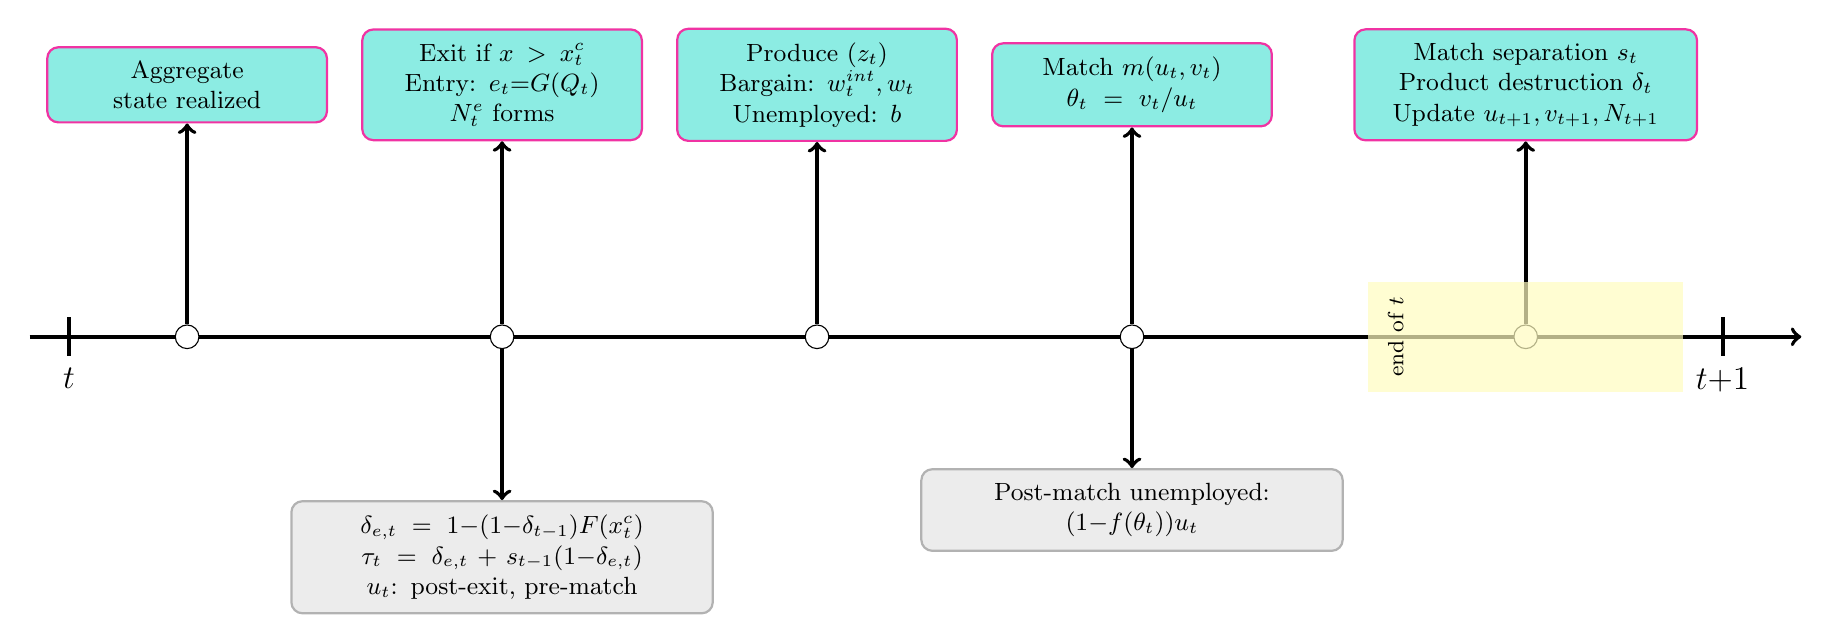
\begin{tikzpicture}[
				box/.style={draw=magenta!80, fill=turquoise!60, thick, rounded corners,
					align=center, font=\small, inner sep=5pt, text width=3.2cm},
				ebox/.style={draw=magenta!80, fill=turquoise!60, thick, rounded corners,
					align=center, font=\small, inner sep=5pt, text width=4.0cm},
				gbox/.style={draw=gray!60, fill=gray!15, thick, rounded corners,
					align=center, font=\small, inner sep=5pt, text width=5cm},
				dot/.style={circle, draw=black, fill=white, inner sep=0pt, minimum size=3mm},
				lw/.style={line width=0.5mm}]
				
				%% ── timeline ──
				\draw[lw,->] (-0.5,0) -- (22,0);
				\draw[lw] (0, 0.25) -- (0,-0.25) node[below]{\large$t$};
				\draw[lw] (21,0.25) -- (21,-0.25) node[below]{\large$t{+}1$};
				
				%% ── dots ──
				\node[dot] (d1) at (1.5,0) {};
				\node[dot] (d2) at (5.5,0) {};
				\node[dot] (d3) at (9.5,0) {};
				\node[dot] (d4) at (13.5,0) {};
				\node[dot] (d5) at (18.5,0) {};
				
				%% ── ABOVE: actions (alternating heights to avoid crowding) ──
				\node[box] (B1) at (1.5, 3.2)
				{Aggregate state realized};
				
				\node[box] (B2) at (5.5, 3.2)
				{Exit if $x>x_t^c$\\Entry: $e_t{=}G(Q_t)$\\$N_t^e$ forms};
				
				\node[box] (B3) at (9.5, 3.2)
				{Produce ($z_t$)\\Bargain: $w_t^{int},w_t$\\Unemployed: $b$};
				
				\node[box] (B4) at (13.5, 3.2)
				{Match $m(u_t,v_t)$\\$\theta_t=v_t/u_t$};
				
				\node[ebox] (B5) at (18.5, 3.2)
				{Match separation $s_t$\\Product destruction $\delta_t$\\
					Update $u_{t+1},v_{t+1},N_{t+1}$};
				
				%% ── BELOW: key implied stocks ──
				\node[gbox] (C1) at (5.5, -2.8)
				{$\delta_{e,t}=1{-}(1{-}\delta_{t-1})F(x_t^c)$\\
					$\tau_t=\delta_{e,t}+s_{t-1}(1{-}\delta_{e,t})$\\
					$u_t$: post-exit, pre-match};
				
				\node[gbox] (C2) at (13.5, -2.2)
				{Post-match unemployed:\\$(1{-}f(\theta_t))u_t$};
				
				%% ── connectors ──
				\foreach \d/\B in {d1/B1, d2/B2, d3/B3, d4/B4, d5/B5}
				\draw[lw,->] (\d) -- (\B);
				
				\draw[lw,->] (d2) -- (C1);
				\draw[lw,->] (d4) -- (C2);
				
				%% ── end-of-period shaded band ──
				\fill[yellow!25, opacity=0.7] (16.5,-0.7) rectangle (20.5,0.7);
				\node[font=\footnotesize, rotate=90] at (16.85,0) {end of $t$};
				
		\end{tikzpicture}}
		\caption{Timing. Turquoise: agent decisions. Grey: implied states. 
			Yellow band: shocks realizing end of $t$, governing $t{+}1$.}
		\label{fig:Timing}
	\end{figure}
	
	%%%%%%%%%%%%%%%%%%%%%%%%%%%%%%%%%%%%%%%%%%
	\section{Equilibrium}\label{sec:equilibrium}
	%%%%%%%%%%%%%%%%%%%%%%%%%%%%%%%%%%%%%%%%%%
	
	This section derives equilibrium given the environment of 
	Section~\ref{sec:environment}. Table~\ref{tab:ingredients_comparison} 
	positions the paper relative to the closest antecedents across 
	four model dimensions. Equilibrium comprises three blocks: a 
	business formation block governing the evolution of product lines 
	and firm values, a labor market block governing vacancy creation, 
	matching, and wage determination, and stochastic processes for 
	the three structural shocks. Section~\ref{sec:mechanism} derives 
	formally the asymmetric transmission of $\delta$ and $s$ shocks 
	that motivates the paper's empirical strategy.
	
	\begin{table}[H]
		\centering
		\footnotesize
		\setlength{\tabcolsep}{0.15cm}
		\begin{tabular}{l|cccc}
			\toprule
			& \makecell{Finitely elastic\\ vacancies} 
			& \makecell{Endogenous\\variety} 
			& \makecell{Endogenous\\separation} 
			& \makecell{Separate destruction\\margin} \\
			\midrule
			Bilbiie, Ghironi, and Melitz (2012) 
			& NA & \checkmark & NA & NA \\
			Coles and Kelishomi (2018) 
			& \checkmark & $\times$ & $\times$ & $\times$ \\
			Broer, Druedahl, Harmenberg, and \"{O}berg (2025) 
			& \checkmark & $\times$ & \checkmark & $\times$ \\
			Gabrovski and Silva (2025) 
			& \checkmark & $\times$ & $\times$ & \checkmark \\
			Shao and Silos (2013) 
			& \checkmark & \checkmark & $\times$ & $\times$ \\
			%Schaal and Taschereau-Dumouchel (2019) 
			%& $\times$ & \checkmark & $\times$ & $\times$ \\
			Christiano, Eichenbaum, and Trabandt (2016) 
			& $\times$ & $\times$ & $\times$ & $\times$ \\
			Colciago, Fasani, and Rossi (2021) 
			& $\times$ & \checkmark & $\times$ & $\times$ \\
			Cacciatore and Fiori (2016) 
			& $\times$ & \checkmark & \checkmark & $\times$ \\
		%	Schaal (2017) 
		%	& $\times$ & $\times$ & \checkmark & $\times$ \\
			\textbf{This paper} 
			& \checkmark & \checkmark & \checkmark & \checkmark \\
			\bottomrule
		\end{tabular}
		\caption{Comparison of model ingredients. 
			\emph{Finitely elastic vacancies}: sunk vacancy creation 
			costs generating a positive vacancy value. 
			\emph{Endogenous variety}: equilibrium number of product 
			lines responds to economic conditions. 
			\emph{Endogenous separation}: firm exit driven by 
			idiosyncratic profitability draws. 
			\emph{Separate destruction margin}: exogenous product-line 
			destruction distinguished from match separation.}
		\label{tab:ingredients_comparison}
	\end{table}
	
	\subsection{Household problem}
	
	Let $\nu_t$ denote the ex-dividend equity price of the aggregate 
	firm portfolio and $\nu_t^f$ the post-dividend value of an 
	individual firm, following \citet{bilbiie_2012}. Given 
	risk-aversion parameter $\sigma$ and discount factor $\beta$, 
	the household chooses consumption $c_t$ and equity shares $a_t$ 
	to maximize expected discounted utility:
	\begin{align}
		\max_{c_t,\,a_t}\sum_{t=0}^{\infty}
		\mathbb{E}_0\,\beta^t c_t^{1-\sigma}/(1-\sigma)
	\end{align}
	subject to
	\begin{align}\label{eq:bc_HH}
		c_t + \nu_t a_{t+1} = w_t(1-u_t) + b u_t 
		+ (\nu_t+d_t)a_t + D_t^{int} - T_t
	\end{align}
	where $b$ is the value of unemployment, $d_t$ is the per-share 
	dividend, $D_t^{int}$ are intermediary dividends, and $T_t$ are 
	lump-sum taxes financing unemployment benefits. Since households 
	have unit mass, $c_t = C_t$ in equilibrium. The first-order 
	condition for equity shares yields the standard asset-pricing 
	equation:
	\begin{align}\label{eq:euler_shares}
		\lambda_t \nu_t = \beta\,\mathbb{E}_t\lambda_{t+1}
		[\nu_{t+1}+d_{t+1}]
	\end{align}
	where $\lambda_t = c_t^{-\sigma}$ is the marginal utility of 
	consumption and $m_{t+1}\equiv\beta(\lambda_{t+1}/\lambda_t)$ 
	is the stochastic discount factor. To express~\eqref{eq:euler_shares} 
	at the firm level, use the mappings $\nu_t=\nu_t^f(N_t+N_t^e)$ 
	and $\nu_t+d_t=(\nu_t^f+d_t^f)N_t$, together with the firm law 
	of motion~\eqref{eq:firm_law_motion}. This yields the firm-level 
	Euler equation, familiar from BGM and extended here to 
	incorporate endogenous exit:
	\begin{align}\label{eq:euler_firm}
		\nu_t^f = \mathbb{E}_t m_{t+1}(1-\delta_t)F(x_{t+1}^c)
		(\nu_{t+1}^f+d_{t+1}^f)
	\end{align}
	Equation~\eqref{eq:euler_firm} equates the current firm value to 
	the expected discounted sum of next-period firm value and 
	dividends, adjusted for the stochastic discount factor 
	$m_{t+1}$ and the survival probability $(1-\delta_t)F(x_{t+1}^c)$, 
	which combines the probability of surviving exogenous destruction 
	$(1-\delta_t)$ and the probability of drawing a continuation 
	cost below the equilibrium cutoff $F(x_{t+1}^c)$.
	
	\subsection{Recruiters}
	\label{sec:recruiters}
	
	There is a fixed unit measure of recruiters who can create 
	vacancies subject to a sunk cost $x$ drawn from cdf $G(\cdot)$. 
	Additionally, if a vacancy is filled the recruiter pays a fixed 
	real cost $\kappa$ before bargaining with the newly matched 
	worker.\footnote{\citet{pissarides_2009} first suggested this 
		matching cost to make vacancy posting more responsive; 
		\citet{christiano_2016} estimate it accounts for the dominant 
		share of recruiting costs.} After matching, the recruiter rents 
	labor to an incumbent retailer with product line $j$. We 
	introduce recruiters as a separate agent type to avoid the 
	complications of Stole-Zwiebel intra-firm bargaining that arise 
	when workers negotiate directly with retailers facing a downward-
	sloping demand curve: with a separate recruiter, the bilateral 
	bargaining problem reduces to the standard DMP surplus-splitting 
	equation regardless of the retail market structure.\footnote{Under 
		Stole-Zwiebel bargaining, retailers would strategically over-hire 
		to improve their bargaining position, generating a fixed-point 
		problem in employment that significantly complicates aggregation. 
		The recruiter segmentation is isomorphic to the retailer--
		wholesaler structure of \citet{christiano_2016}, with recruiters 
		replacing intermediate goods.} Let $Q_t^j$ and $J_t^j$ denote 
	the values of an unfilled and filled vacancy associated with 
	product line $j$.
	
	The value of an unfilled vacancy for product line $j$ satisfies
	\begin{align}\label{eq:value_recruiter_unmatched}
		Q_{t}^j &= \mathbb{E}_t m_{t+1}(1-\delta_t)F(x_{t+1}^c)
		\bigl[(1-q(\theta_t))Q_{t+1}^j
		+q(\theta_{t})J_{t+1}^j\bigr]-q(\theta_t)\kappa \notag \\
		&= \mathbb{E}_t m_{t+1}(1-\delta_t)F(x_{t+1}^c)
		\bigl[Q_{t+1}^j+q(\theta_t)
		(J_{t+1}^j-Q_{t+1}^j)\bigr]-q(\theta_t)\kappa
	\end{align}
	An unmatched recruiter survives to next period only if the 
	product line survives both exogenous destruction and the 
	continuation-cost draw, with probability $(1-\delta_t)F(x_{t+1}^c)$. 
	In the next period, the vacancy fills with probability 
	$q(\theta_t)$, generating value $J_{t+1}^j$, or remains unfilled 
	with probability $1-q(\theta_t)$. The matching cost $\kappa$ 
	is paid upon filling. The recruiter chooses the best product 
	line: $Q_t\equiv\max_j Q_t^j$. In equilibrium, competition 
	equalizes values across active product lines: $Q_t^j=Q_t$ for 
	all $j$ with $v_t^j>0$.
	
	Define the flow value of a vacancy as the net benefit of 
	holding a vacancy this period relative to next:
	\begin{align}\label{eq:K}
		K_t \equiv Q_t - 
		\mathbb{E}_t m_{t+1}(1-\delta_t)F(x_{t+1}^c)Q_{t+1}
	\end{align}
	Rearranging~\eqref{eq:value_recruiter_unmatched} places the 
	average hiring cost on the left-hand side:
	\begin{align}\label{eq:average_hiring_cost}
		\kappa+\frac{K_t}{q(\theta_t)} = 
		\mathbb{E}_t m_{t+1}(1-\delta_t)F(x_{t+1}^c)
		(J_{t+1}^j-Q_{t+1})
	\end{align}
	
	A recruiter opens a vacancy whenever $x\leq Q_t$, so total 
	newly opened vacancies are $e_t=G(Q_t)$. Following CK, we 
	adopt a power law distribution:
	\begin{align}
		G(x)=\left(\frac{x}{x_m}\right)^{\xi}, 
		\quad x\in[0,\,x_m]
	\end{align}
	with density $g(x)=\xi x^{\xi-1}/x_m^{\xi}$.\footnote{If 
		$\xi>1$ the density is rising (relatively more high-cost 
		recruiters); if $\xi<1$ it is falling; if $\xi=1$ costs are 
		uniform on $[0,x_m]$.} Provided $Q<x_m$, inverting $e=G(Q)$ 
	gives
	\begin{align}\label{eq:Q}
		Q_t = e_t^{1/\xi}\,x_m
	\end{align}
	so the elasticity of the vacancy value with respect to entry 
	is $1/\xi$. Free entry of vacancies ($\xi\to\infty$) nests 
	the DMP baseline.
	
	By symmetry of the retail problem (established in 
	Section~\ref{sec:retailers}), recruiter compensation 
	$w_t^{int,j}$ and the value of a filled vacancy $J_t^j$ are 
	identical across active product lines; we henceforth drop the 
	superscript $j$. Recruiters supply labor in a competitive 
	market, taking $w_t^{int}$ as given. The value of a matched 
	recruiter is\footnote{The asset-pricing equations 
		\eqref{eq:value_recruiter_unmatched} and 
		\eqref{eq:value_recruiter_matched} can equivalently be obtained 
		by having the household purchase shares of recruiter firms 
		directly; the stochastic discount factor ensures equivalence. 
		Writing it via the household problem makes the derivation more 
		compact and facilitates comparison to BGM and 
		\citet{mortensen_1994}.}
	\begin{align}\label{eq:value_recruiter_matched}
		J_{t} = w_t^{int}-w_t + \mathbb{E}_{t}m_{t+1}
		(1-\delta_t)F(x_{t+1}^c)
		\bigl(s_t Q_{t+1}+(1-s_t)J_{t+1}\bigr)
	\end{align}
	The recruiter receives $w_t^{int}$ from the retailer and 
	pays the worker $w_t$. Conditional on product-line survival, 
	the match continues with probability $1-s_t$; otherwise the 
	vacancy is reposted at no additional sunk cost.
	
	\paragraph{Job creation condition.}
	Subtracting~\eqref{eq:value_recruiter_unmatched} 
	from~\eqref{eq:value_recruiter_matched} and using the definition 
	of $K_t$ yields recruiter surplus:
	\begin{align}\label{eq:value_recruiter_surplus}
		J_t - Q_t &= w_t^{int}-w_t - K_t 
		+ (1-s_t)\left(\kappa+\frac{K_t}{q(\theta_t)}\right)
	\end{align}
	Substituting~\eqref{eq:value_recruiter_surplus} into the 
	right-hand side of~\eqref{eq:average_hiring_cost} yields the 
	job creation condition:
	\begin{align}\label{eq:jcc}
		\kappa+\frac{K_t}{q(\theta_t)} = 
		\mathbb{E}_t m_{t+1}(1-\delta_{t})F(x_{t+1}^c)
		\left(w_{t+1}^{int}-w_{t+1}-K_{t+1}
		+(1-s_{t+1})\left(\kappa+\frac{K_{t+1}}{q(\theta_{t+1})}
		\right)\right)
	\end{align}
	The left-hand side is the average hiring cost: the fixed 
	matching cost $\kappa$ plus the flow cost $K_t/q(\theta_t)$, 
	equal to the opportunity cost of holding the vacancy this 
	period multiplied by its expected duration $1/q(\theta_t)$. 
	The right-hand side is the present discounted value of the 
	match: future net revenue minus the future flow entry cost, 
	plus the continuation value if the worker is retained, 
	discounted by the stochastic discount factor and the 
	product-line survival probability.
	
	\subsection{Wage determination}
	
	Nash bargaining between the recruiter and worker yields
	\begin{align}\label{eq:wage_eq}
		w_t = \phi\left(w_t^{int} - K_t 
		+ f(\theta_t)\left(\kappa
		+\frac{K_t}{q(\theta_t)}\right)\right)
		+(1-\phi)b
	\end{align}
	where $\phi$ is the worker's bargaining power.\footnote{The 
		wage equation \eqref{eq:wage_eq} has the same general form as 
		\citet{shao_2013}, their equations 21 and 22; their setting 
		includes capital affecting $w_t^{int}$ and writes the wage 
		using the vacancy value $Q_t$ rather than the flow value 
		$K_t$.} Recruiter compensation $w_t^{int}=\rho(N_t)z_t/
	\mu(N_t)$ — derived in Section~\ref{sec:retailers} — enters 
	negatively through the markup. The flow entry cost $K_t$ has 
	opposing effects: it reduces the match surplus (dampening 
	wages by $\phi K_t$) but improves the worker's threat point, 
	raising the tightness slope of the wage curve by $\phi\theta 
	K_t$; the second effect dominates when $\theta>1$. The fixed 
	cost $\kappa$ raises wages by $\phi f(\theta_t)\kappa$ because 
	a failed negotiation forces the firm to pay $\kappa$ again 
	upon next filling the vacancy. Setting $w_t^{int}=z_t$ and 
	$\kappa=0$ recovers the CK wage equation.
	
	Substituting~\eqref{eq:wage_eq} into~\eqref{eq:jcc} to 
	eliminate $w_t$ yields the wage-substituted job creation 
	condition:
	\begin{align}\label{eq:jcc_wage}
		\kappa+\frac{K_t}{q(\theta_t)} = 
		\mathbb{E}_t m_{t+1}(1-\delta_{t})F(x_{t+1}^c)
		\Biggl[&(1-\phi)\left(w_{t+1}^{int}
		-K_{t+1}-b\right) \notag \\
		&-\phi\theta_{t+1}\left(K_{t+1}
		+q(\theta_{t+1})\kappa\right) \notag \\
		&+(1-s_{t+1})\left(\kappa
		+\frac{K_{t+1}}{q(\theta_{t+1})}\right)
		\Biggr]
	\end{align}
	
	\subsection{Retailers}\label{sec:retailers}
	
	A retailer selling variety $j$ rents labor from recruiters at 
	wage $w_t^{int,j}$. At the beginning of each period, before 
	production, the firm draws a continuation cost $\chi\sim F_\chi$ 
	in units of the consumption basket, where $F_\chi$ is a mixture 
	between a mass point at zero with probability $1-p_0$ and a 
	bounded power law:
	\begin{align}\label{eq:F_chi}
		F_\chi(\chi) = (1-p_0) + p_0\left(\frac{\chi}{\chi_m}
		\right)^\psi, 
		\quad \chi\in[0,\,\chi_m]
	\end{align}
	A firm with draw $\chi>\chi_t^c$ exits; one with $\chi\leq\chi_t^c$ 
	pays the cost and continues. Define the survival probability:
	\begin{align}\label{eq:Lambda}
		\Lambda_t \equiv F_\chi(\chi_t^c) = (1-p_0) 
		+ p_0\left(\frac{\chi_t^c}{\chi_m}\right)^\psi
	\end{align}
	so that the endogenous exit rate is $1-\Lambda_t = 
	p_0\left(1-(\chi_t^c/\chi_m)^\psi\right)$, consistent with the 
	total exit rate $\delta_{e,t}=1-(1-\delta_{t-1})\Lambda_t$ from 
	Section~\ref{sec:environment}. The elasticity of the endogenous 
	exit rate with respect to the cutoff is 
	$\psi p_0(\chi_t^c/\chi_m)^\psi/(1-\Lambda_t)$, which increases 
	in $\psi$ and falls as the mass point $1-p_0$ rises.
	
	The value of a firm after its cost realization is:
	\begin{align}\label{eq:firm_bellman}
		\nu_t^f(\chi) = \max\left\{0,\; 
		\max_{y_t}\left[\rho^d(y_t)y_t - 
		w_t^{int}\frac{y_t}{z_t}\right]
		-\chi + (1-\delta_t)\mathbb{E}_t m_{t+1}\Lambda_{t+1}
		\,\nu_{t+1}^{ef}\right\}
	\end{align}
	where $\nu_t^{ef}\equiv(1/\Lambda_t)\int_0^{\chi_t^c}
	\nu_t^f(\tilde{\chi})\,dF_\chi(\tilde{\chi})$ is the expected 
	firm value conditional on survival, and $\rho^d(y_t)$ is the 
	inverse demand curve from~\eqref{eq:demand}, equal in symmetric 
	equilibrium to $\rho(N_t)$. The profit maximization problem 
	is static: letting $MR\equiv\rho'(y)y+\rho(y)$ denote marginal 
	revenue, the first-order condition is
	\begin{align}\label{eq:retailer_optimality}
		MR_t\cdot z_t = w_t^{int,j}
	\end{align}
	The left-hand side is the marginal revenue product; the 
	right-hand side is recruiter compensation, which exceeds the 
	worker's wage due to matching frictions. Equivalently, 
	$MR_t = MC_t = w_t^{int}/z_t$. The standard markup condition 
	$\rho_t = \mu(N_t)MC_t$ gives recruiter compensation:
	\begin{align}\label{eq:recruiter_compensation}
		w_t^{int} = \frac{\rho(N_t)}{\mu(N_t)}z_t
	\end{align}
	Recruiter compensation is increasing in the relative price 
	$\rho(N_t)$ and technology $z_t$ and decreasing in the markup 
	$\mu(N_t)$. Since $\mu'(N_t)\leq 0$, $w_t^{int}$ is 
	increasing in $N_t$ overall.\footnote{Following BGM, marginal 
		cost is $w_t^{int}/z_t$. Under DS-CES, $\mu=\varepsilon/
		(\varepsilon-1)$ is constant, recovering the standard formula.} 
	Retail profits gross of the continuation cost are a share 
	$(\mu(N_t)-1)/\mu(N_t)$ of sales:
	\begin{align}\label{eq:retail_profits}
		R_t^f = \frac{\mu(N_t)-1}{\mu(N_t)}\rho(N_t)y_t
	\end{align}
	
	\subsection{Firm entry and exit}\label{sec:entry_exit}
	
	By definition $\nu_t^f(\chi_t^c)=0$. Evaluating 
	the firm Bellman~\eqref{eq:firm_bellman} at 
	$\chi=\chi_t^c$ yields the cutoff condition:
	\begin{align}\label{eq:cutoff}
		\chi_t^c = R_t^f + \nu_t^f
	\end{align}
	where $\nu_t^f\equiv\nu_t^{ef}\cdot\Lambda_t$ is the 
	unconditional expected firm value. From the Bellman, 
	the firm value conditional on the cost realization is 
	$\nu_t^f(\chi)=\chi_t^c-\chi$ for all $\chi\leq\chi_t^c$, 
	so that $\nu_t^{ef}=\chi_t^c - E(\chi\,|\,\chi\leq\chi_t^c)$. 
	For the power law component, the conditional mean of a 
	positive draw satisfies $E(\chi\,|\,0<\chi\leq\chi_t^c)
	=\psi_c\chi_t^c$ where $\psi_c\equiv\psi/(\psi+1)$, 
	so the overall conditional mean (including the mass point 
	at zero) is $E(\chi\,|\,\chi\leq\chi_t^c)=p_0\psi_c\chi_t^c$. 
	Hence:
	\begin{align}\label{eq:firm_value_char}
		\nu_t^f = (1-\delta_t)\mathbb{E}_t m_{t+1}
		\Lambda_{t+1}\,\nu_{t+1}^{ef}
	\end{align}
	
	New firms are created using technology $N_t^e=z_t l_t^e/f_e$, 
	where $l_t^e$ is labor hired from recruiters at wage 
	$w_t^{int}$ and $f_e$ is the sunk entry cost in labor units, 
	equivalent to $w_t^{int}f_e/z_t=\rho(N_t)f_e/\mu(N_t)$ 
	units of the consumption basket. Firms enter until the 
	post-dividend firm value equals the sunk entry cost:
	\begin{align}\label{eq:free_entry}
		\nu_t^f = \frac{\rho(N_t)f_e}{\mu(N_t)}
	\end{align}
	Combining the free entry condition~\eqref{eq:free_entry} 
	with the cutoff condition~\eqref{eq:cutoff} yields:
	\begin{align}\label{eq:cutoff_free_entry}
		\chi_t^c = R_t^f + \frac{\rho(N_t)f_e}{\mu(N_t)}
	\end{align}
	The cutoff rises with current profitability $R_t^f$ and 
	the value of a new product line $\rho(N_t)f_e/\mu(N_t)$: 
	when conditions improve, marginal firms that would 
	otherwise exit find it worthwhile to continue.
	\subsection{Aggregation}\label{sec:aggregation}
	
	Labor market clearing implies $L_t = 1-u_t$. Define 
	gross consumption output $Y_t^c \equiv \rho(N_t)N_t y_t$ 
	and retail employment $L_t^c \equiv N_t l_t^c$. Aggregate 
	continuation costs paid by surviving firms are
	\begin{align}\label{eq:agg_fixed_costs}
		X_t^c \equiv N_t\,E(\chi\,|\,\chi\leq\chi_t^c) 
		= N_t p_0\psi_c\chi_t^c
	\end{align}
	where $\psi_c\equiv\psi/(\psi+1)$. Aggregate retail profits 
	gross of continuation costs are $\Pi_t^f = Y_t^c/
	\varepsilon(N_t) - X_t^c$, and recruiter profits are 
	$\Pi_t^{int} = (w_t^{int}-w_t)L_t$. The average per-firm 
	dividend is $d_t^f = \Pi_t^f/N_t$.
	
	Total vacancy creation costs are the sum of sunk posting 
	costs and fixed matching costs:
	\begin{align}\label{eq:X_total}
		X_t = X_v + X_f 
		= e_t\frac{\xi}{\xi+1}Q_t + \kappa q(\theta_t)v_t
	\end{align}
	where $X_v = x_m^{-\xi}\frac{\xi}{\xi+1}Q_t^{\xi+1}$ 
	follows from integrating $xg(x)$ over $[0,Q_t]$. Given 
	$e_t$ and $Q_t$, the parameter $x_m$ has no additional 
	effect on entry costs provided $Q_t < x_m$.
	
	Aggregating~\eqref{eq:bc_HH} with asset market clearing 
	$a_{t+1}=a_t$ and $T_t=bu_t$, and using 
	$Y_t^{Gross} = Y_t^c + \nu_t^f N_t^e$, real GDP net 
	of intermediate inputs is:
	\begin{align}\label{eq:gdp}
		Y_t \equiv Y_t^{Gross} - X_t - X_t^c 
		= C_t + \nu_t^f N_t^e 
		= w_tL_t + \Pi_t^f + \Pi_t^{int}
	\end{align}
	GDP comprises consumption and investment in new product 
	lines. Moreover, decomposing output into income confirms the national 
	accounts identity.
	
	Using free entry~\eqref{eq:free_entry} and $d_t^f = 
	\Pi_t^f/N_t$, the firm-level Euler 
	equation~\eqref{eq:euler_firm} becomes the business 
	formation equation:
	\begin{align}\label{eq:euler_bf}
		f_e\rho(N_t) = (1-\delta_t)\mathbb{E}_t m_{t+1}
		\Lambda_{t+1}\frac{\mu(N_t)}{\mu(N_{t+1})}
		\left\{f_e\rho(N_{t+1}) + \frac{Y_{t+1}^c}{N_{t+1}}
		\left(\mu(N_{t+1})-1-\mu(N_{t+1})
		\frac{X_{t+1}^c}{Y_{t+1}^c}\right)\right\}
	\end{align}
	The left-hand side is the current cost of creating a 
	product line. The right-hand side is the expected 
	discounted return, adjusted for survival probability 
	$(1-\delta_t)\Lambda_{t+1}$ and the current-to-future 
	markup ratio $\mu(N_t)/\mu(N_{t+1})$. The term in 
	braces is the next-period firm value plus the private 
	marginal product of a new product line net of 
	continuation costs; the net markup $\mu(N_{t+1})-1$ 
	governs the return to entry.
	
	\subsection{Definition of equilibrium}\label{sec:def_eq}
	
	\begin{definition}\label{def:equilibrium}
		Given $\rho(N)$, $\mu(N)$, $F_\chi$, initial exogenous 
		states $\{z_0,\delta_0,s_0\}$, and initial endogenous 
		states $\{v_{-1},u_{-1},u_0,N_0\}$, an equilibrium is 
		a sequence $\{N_t, C_t, \chi_t^c, Y_t^c, \theta_t, 
		K_t, Q_t, e_t, v_t, u_t\}_{t=0}^\infty$ satisfying the 
		business formation block:
		\begin{align}
			\label{eq:N_lom_eq}
			N_t &= (1-\delta_{t-1})\Lambda_t
			\left(N_{t-1} + \frac{z_{t-1}(1-u_{t-1})}{f_e} 
			- \frac{Y_{t-1}^c}{f_e\rho(N_{t-1})}\right) \\
			\label{eq:N_euler_eq}
			f_e\rho(N_t) &= (1-\delta_t)\mathbb{E}_t 
			m_{t+1}\Lambda_{t+1}
			\frac{\mu(N_t)}{\mu(N_{t+1})}
			\left\{f_e\rho(N_{t+1}) + \frac{Y_{t+1}^c}{N_{t+1}}
			\left(\mu(N_{t+1})-1-\mu(N_{t+1})
			\frac{X_{t+1}^c}{Y_{t+1}^c}\right)\right\} \\
			\label{eq:rc}
			Y_t^c &= C_t + X_t + X_t^c \\
			\label{eq:cutoff_eq}
			\chi_t^c &= \frac{Y_t^c(\mu(N_t)-1)}{\mu(N_t)N_t} 
			+ \frac{f_e\rho(N_t)}{\mu(N_t)}
		\end{align}
		and the labor market block:
		\begin{align}
			\label{eq:jcc_eq}
			\kappa+\frac{K_t}{q(\theta_t)} &= 
			\mathbb{E}_t m_{t+1}(1-\delta_t)\Lambda_{t+1}
			\left((1-\phi)\left(\frac{\rho(N_{t+1})z_{t+1}}
			{\mu(N_{t+1})}-K_{t+1}-b\right) \right. \notag \\
			&\quad\left. -\,\phi\theta_{t+1}
			\left(K_{t+1}+q(\theta_{t+1})\kappa\right)
			+(1-s_{t+1})\left(\kappa
			+\frac{K_{t+1}}{q(\theta_{t+1})}\right)\right) \\
			\label{eq:Kdef}
			K_t &= Q_t - (1-\delta_t)\mathbb{E}_t 
			m_{t+1}\Lambda_{t+1}Q_{t+1} \\
			\label{eq:entry_eq}
			e_t &= \left(\frac{Q_t}{x_m}\right)^\xi
		\end{align}
		together with laws of motion 
		\eqref{eq:v_lom}--\eqref{eq:u_lom}, auxiliary 
		definitions $\delta_{e,t}$ \eqref{eq:delta_e_lom}, 
		$\tau_t$ \eqref{eq:tau_lom}, $\Lambda_t$ 
		\eqref{eq:Lambda}, $X_t$ \eqref{eq:X_total}, $X_t^c$ 
		\eqref{eq:agg_fixed_costs}, $m_t$ \eqref{eq:euler_shares}, and 
		stochastic processes \eqref{eq:ar1_z}--\eqref{eq:ar1_s}.
	\end{definition}
	
	The business formation block jointly 
	determines $N_t$, $C_t$, $Y_t^c$, and $\chi_t^c$: 
	the firm LOM propagates the product-line stock, the 
	business formation Euler governs entry, the resource 
	constraint clears goods markets, and the cutoff equates 
	the exit threshold to current profitability plus the 
	option value of a new product line. The labor market 
	block jointly 
	determines $u_t, v_t, \theta_t$, $K_t$, and $Q_t$: the job 
	creation condition equates average hiring cost to the 
	present discounted value of a filled vacancy, and free 
	entry pins down the vacancy creation margin. The two 
	blocks interact through $\rho(N_t)$ and $\mu(N_t)$ 
	in the job creation condition and through $\delta_t$ 
	in the survival-adjusted discount factor 
	$(1-\delta_t)\Lambda_{t+1}$, which appears in both.

\subsection{Limiting cases}

The next several propositions characterize the 
relationship between the business formation block 
and labor market block, and establish the connection 
to benchmark frameworks in the literature. Proofs 
are in \ref{app:limiting_cases}.

\begin{proposition}[Independence of labor market block]
	\label{prop:independence}
	Consider general CES preferences with elasticity of 
	substitution $\varepsilon$ held fixed. The labor market 
	block $\{u_{t+1}, v_t, e_t, Q_t, K_t, w_t\}_{t=0}^{\infty}$ 
	can be solved independently of the business formation 
	block if and only if $\sigma=0$, $\zeta=0$, and $p_0=0$.
\end{proposition}

When $\sigma=0$, risk neutrality fixes $m_{t+1}=\beta$, 
eliminating the consumption dependence of the stochastic 
discount factor. When $\zeta=0$, the taste for variety 
vanishes and $\rho(N_t)=1$, removing $N_t$ from recruiter 
compensation $w_t^{int}=\rho(N_t)z_t/\mu(N_t)$ and from 
the job creation condition while leaving $\mu$ and hence 
the business formation block otherwise intact. When 
$p_0=0$, endogenous exit is absent so $\Lambda_t=1$ and 
$\delta_{e,t}=\delta_{t-1}$ depends only on the exogenous 
shock. Under all three conditions, the labor market block 
closes on its own; the business formation block then 
determines $C_t$ and $N_t$ taking $u_t$ and $X_t$ as 
given from the labor market block.

The model nests GS and CK as the taste for variety 
vanishes, which under DS-CES corresponds to 
$\varepsilon\to\infty$. This limit is not directly 
workable, however: with $f_e$ fixed, vanishing profits 
($\mu\to 1$) make entry unprofitable and $N\to 0$ from 
the resource constraint, so that $Y_t^c=\rho(N_t)N_t y_t
\to 0$ with positive employment, rendering aggregate 
production degenerate. One might restore a non-degenerate 
limit by setting $\delta\to 0$, but this would eliminate 
the destruction margin that is central to the vacancy 
law of motion in GS and CK --- precisely the channel we 
wish to preserve. We instead seek a joint limit in which 
entry costs shrink proportionally with profits, keeping 
the product-line stock well-defined and positive while 
making business formation irrelevant to aggregate labor 
market allocations. Proposition~\ref{prop:double_limit} 
shows that scaling $f_e=\bar{f}_e/\varepsilon$ jointly 
with $\varepsilon\to\infty$ achieves exactly this.

\begin{proposition}[Double limit]
	\label{prop:double_limit}
	Consider DS-CES preferences. Set $p_0=0$, and let 
	$\varepsilon\to\infty$ jointly with $f_e=\bar{f}_e/
	\varepsilon$ for fixed $\bar{f}_e>0$. Then: \emph{(i)} the product-line mass has a unique 
	positive steady-state value $\bar{N}>0$ satisfying 
	$\bar{\delta}\bar{N} = \bar{z}\bar{L}\ln\bar{N}/
	\bar{f}_e$; local stability of the $N_t$ dynamics 
	around $\bar{N}$ holds provided 
	$\bar{N}>e^{1-\bar{\delta}}$, a condition satisfied 
	for sufficiently small $\bar{f}_e$ given other 
	parameters. \emph{(ii)} firm 
	value $\nu_t^f$, investment $\nu_t^f N_t^e$, and 
	labor devoted to entry $l_t^e$ all vanish at rate 
	$1/\varepsilon$; \emph{(iii)} recruiter compensation 
	$w_t^{int}\to z_t$; and \emph{(iv)} aggregate 
	allocations $\{\theta_t, u_t, v_t, C_t, Y_t^c\}$ 
	are independent of $\bar{N}$, so the normalization 
	$\bar{N}=1$ is without loss of generality for 
	aggregate allocations. In the limit, the business 
	formation block is irrelevant to real allocations.
\end{proposition}

As $\varepsilon\to\infty$ under DS-CES, 
$\zeta=1/(\varepsilon-1)\to 0$, satisfying one of 
the separability conditions of 
Proposition~\ref{prop:independence}. 
Proposition~\ref{prop:double_limit} is stronger, 
however: it establishes not merely that the labor 
market block separates but that business formation 
becomes irrelevant to aggregate allocations entirely 
--- a consequence of profits and entry costs 
vanishing jointly at the same rate. 
Proposition~\ref{prop:ags} below implements the 
limiting economy directly via clone replacement, 
maintaining $N_t=1$ by construction rather than 
through the limit passage.

\begin{proposition}[Clone-replacement equilibrium]
	\label{prop:ags}
	Under clone replacement with $N_t=1$ and $\mu=1$, 
	the business formation block drops out and equilibrium 
	labor market variables 
	$\{u_{t+1},v_t,e_t,Q_t,K_t\}_{t=0}^\infty$ satisfy:
	\begin{align}
		\label{eq:jcc_ags}
		\kappa+\frac{K_t}{q(\theta_t)} &= 
		\mathbb{E}_t m_{t+1}(1-\delta_t)
		\left((1-\phi)(z_{t+1}-K_{t+1}-b) \right.\notag\\
		&\quad\left. -\phi\theta_{t+1}
		(K_{t+1}+q(\theta_{t+1})\kappa)
		+(1-s_{t+1})\left(\kappa+
		\frac{K_{t+1}}{q(\theta_{t+1})}\right)\right)\\
		\label{eq:K_ags}
		K_t &= Q_t-(1-\delta_t)\mathbb{E}_t 
		m_{t+1}Q_{t+1}\\
		\label{eq:v_ags}
		v_t &= (1-\delta_{t-1})
		\left[(1-q(\theta_{t-1}))v_{t-1}
		+s_{t-1}(1-u_{t-1})\right]+e_t\\
		\label{eq:u_ags}
		u_t &= (1-f(\theta_{t-1}))u_{t-1}
		+\tau_t\left[(1-u_{t-1})
		+f(\theta_{t-1})u_{t-1}\right]
	\end{align}
	together with $e_t=G(Q_t)$, 
	$m_t=\beta(C_t/C_{t-1})^{-\sigma}$, 
	$C_t=z_t(1-u_t)-X_t$, and stochastic processes 
	\eqref{eq:ar1_z}--\eqref{eq:ar1_s}, with 
	$\delta_{e,t}=\delta_{t-1}$ since endogenous exit 
	is absent by construction.
\end{proposition}

We dub this the \emph{augmented Gabrovski-Silva} 
(AGS) model. Relative to AGS, the baseline model 
adds two channels affecting labor market dynamics: 
variety effects in the job creation condition 
through $\rho(N_t)/\mu(N_t)$, and endogenous exit 
through variation in the survival cutoff $\chi_t^c$, 
as developed formally in Section~\ref{sec:mechanism} 
and evaluated quantitatively in 
Section~\ref{sec:quantitative}.

\begin{remark}[Nested special cases of AGS]
	\label{rem:nesting}
	The AGS model nests two benchmark frameworks as
	limiting cases. Setting $\sigma=\kappa=0$ renders
	the AGS system isomorphic to \citet{gabrovski_2025},
	extended here with aggregate AR(1) shocks to
	$\delta_t$ and $s_t$.
	Additionally setting $s_t=0$ recovers
	\citet{coles_2018} exactly, with $w_t^{int}=z_t$
	and consumption determined residually from
	$z_t(1-u_t)=C_t+\frac{\xi}{\xi+1}Q_t^{\xi+1}$.
\end{remark}

Strictly speaking, the baseline model does not nest
\citet{bilbiie_2012} since there is no intensive labor
margin.  However, it does nest a restricted version.
Define \emph{labor-restricted BGM} (LR-BGM) as the
\citet{bilbiie_2012} model with labor dropped from
preferences: the household maximizes $\sum_t \beta^t
c_t^{1-\sigma}/(1-\sigma)$ subject to
$c_t = w_t L_t + \pi_t - X_t$, where $\{L_t\}$ and
$\{X_t\}$ are exogenous sequences and $X_t$ is the
vacancy-creation cost absorbed as an intermediate input.
The resource constraint of LR-BGM is therefore
$Y_t = C_t + \nu_t^f N_t^e$, matching the GDP identity
\eqref{eq:gdp}, with $X_t$ netted out on both sides.

\begin{proposition}[Nesting LR-BGM]
	\label{prop:bgm_nest}
	Set $p_0=0$, so $X_t^c=0$, $\Lambda_t=1$, and
	$\delta_{e,t}=\delta_{t-1}$.  For any exogenous
	sequences $\{L_t\}$ and $\{X_t\}$, the business
	formation block of the baseline model---equations
	\eqref{eq:N_lom_eq}, \eqref{eq:N_euler_eq}, and
	\eqref{eq:gdp}---is isomorphic to LR-BGM evaluated
	at the same sequences.
\end{proposition}

The isomorphism holds at the level of GDP \eqref{eq:gdp}
rather than gross output \eqref{eq:rc}: vacancy costs
$X_t$ are intermediate inputs in both models and cancel
from the resource constraint, leaving
$Y_t = C_t + \nu_t^f N_t^e$ in each case.  The sole
departure of the baseline from LR-BGM is that $L_t$ and
$X_t$ are endogenous, determined jointly by the DMP block
\eqref{eq:v_lom}--\eqref{eq:u_lom}.  Restoring $p_0>0$
further adds endogenous exit to the LR-BGM core.

\subsection{Steady state}\label{sec:steady_state}

A steady state is a fixed point of the equilibrium system 
in which all variables are constant and shocks are at their 
long-run means $(\bar{z},\bar{\delta},\bar{s})$. We 
characterize it in two blocks. The \emph{exit block} in 
$(\chi^c, \delta_e)$ space determines the exit threshold 
and total destruction rate given aggregate profitability. 
The \emph{labor market and entry block} in $(\theta, N)$ 
space determines market tightness and product variety given 
$\delta_e$. The two blocks interact through $\delta_e$ and 
$\rho(N)$, and must be solved jointly. We focus on the 
$(\theta, N)$ block for the diagrammatic analysis, treating 
$\delta_e$ as a parameter; the full steady-state system 
and key derivations are in 
\ref{app:steady_state}.

\paragraph{Key steady-state ratios}
Setting $\delta_t = \bar{\delta}$ and $s_t = \bar{s}$, the 
Euler equations yield $N^e/N = \delta_e/(1-\delta_e)$. 
Retail profits as a fraction of consumption output are
\begin{align}\label{eq:profit_share}
	\pi_s \equiv \frac{Nd^f}{Y^c} 
	= \frac{1}{\varepsilon(N)} - \frac{X^c}{Y^c}
\end{align}
The profit share $\pi_s$ captures the net return to 
operating a product line after continuation costs: it 
falls with the elasticity of substitution (competition 
erodes markups) and with the continuation cost burden 
$X^c/Y^c$. The equilibrium relationship between total 
employment and product lines is:
\begin{align}\label{eq:labor_N}
	N = \frac{\pi_s z L (1-\delta_e)}
	{f_e\left(\frac{r+\delta_e}{\mu(N)}
		+\delta_e\pi_s\right)}
\end{align}
At a given profit share, a higher destruction rate 
$\delta_e$ reduces product lines relative to employment 
by raising the effective discount rate on future profits 
and increasing the entry required to maintain the 
product-line stock. The full derivation of steady-state 
output shares and labor allocation is in 
\ref{app:steady_state}.

\paragraph{Four steady-state curves}
The \emph{exit threshold curve} gives the locus 
$(\chi^c, \delta_e)$ consistent with the cutoff 
condition \eqref{eq:cutoff_eq} at steady state:
\begin{align}\label{eq:exit_threshold_curve}
	\chi^c = \frac{\rho(N) f_e}{\mu(N)}
	\left(\frac{r+\delta_e}{1-\delta_e}
	\cdot\frac{r+\delta_e+\psi_c(1-\delta_e)}
	{(1-\psi_c)(r+\delta_e)}+1\right)
\end{align}
A higher destruction rate requires higher per-period 
profits to compensate, raising $\chi^c$; higher variety 
$N$ shifts the curve upward through $\rho(N)$. The 
\emph{product destruction curve} follows from 
$\Lambda(\chi^c)(1-\delta) = (1-\delta_e)$:
\begin{align}\label{eq:destruction_curve}
	\chi^c = \left(\frac{1-\delta_e}{1-\delta}
	\right)^{1/\psi}\chi_m
\end{align}
It is negatively sloped: a higher cutoff $\chi^c$ 
raises the endogenous survival probability and 
therefore lowers $\delta_e$.

For the labor market block, express $e$ and $K$ as 
functions of tightness $\theta$ using the steady-state 
unemployment and vacancy laws of motion:
\begin{align}\label{eq:e_theta}
	e(\theta) = \delta_e\,
	\frac{\tau\theta + (1-\delta_e)f(\theta)}
	{\tau + (1-\delta_e)f(\theta)}, \qquad
	K(\theta) = \frac{r+\delta_e}{1+r}\,
	e(\theta)^{1/\xi}\,x_m
\end{align}
The \emph{job creation curve} is the steady-state JCC 
\eqref{eq:jcc_eq}:
\begin{align}\label{eq:curve_jcc}
	\left(\kappa+\frac{K(\theta)}{q(\theta)}\right)
	\left(r+\tau+(1-\delta_e)\phi\theta q(\theta)\right)
	= (1-\delta_e)(1-\phi)
	\left(\frac{\rho(N)z}{\mu(N)}-K(\theta)-b\right)
\end{align}
Its right-hand side is increasing in $N$ through 
$\rho(N)$: more product lines raise recruiter 
compensation, stimulating vacancy creation --- the 
employment--variety feedback emphasized by 
\citet{schaal_2019} and derived here in a more 
flexible setting. Under general CES with $\zeta=0$, 
$\rho=1$ and \eqref{eq:curve_jcc} determines $\theta$ 
independently of $N$, yielding a vertical line in 
$(\theta,N)$ space. The \emph{resource constraint 
	curve} combines the aggregate resource constraint, 
free entry \eqref{eq:free_entry}, and the $N$-$L$ 
relationship \eqref{eq:labor_N}:
\begin{align}\label{eq:curve_res_cons}
	N = \frac{(\mu(N)-1)zL(\theta)(1-\delta_e)}
	{f_e(\delta_e\mu(N)+r)}
\end{align}
Employment $L(\theta)$ is increasing and concave in 
$\theta$, so \eqref{eq:curve_res_cons} is increasing, 
concave, and bounded above by 
$\bar{N}=(\mu-1)z(1-\delta_e)/(f_e(\delta_e\mu+r))$, 
the product variety consistent with full employment.

\begin{proposition}[Variety effects and elasticity 
	of substitution]\label{prop:curves}
	The exit threshold curve \eqref{eq:exit_threshold_curve}, 
	job creation curve \eqref{eq:curve_jcc}, and resource 
	constraint curve \eqref{eq:curve_res_cons} each depend 
	on the elasticity of substitution $\varepsilon(N)$. Only 
	the exit threshold and job creation curves depend on 
	the benefit of variety $\zeta(N)$. The product 
	destruction curve \eqref{eq:destruction_curve} is 
	independent of both.
	
\end{proposition}

The result follows directly from the expressions above: 
$\varepsilon(N)$ enters $\mu(N)$ and $\pi_s$ in all 
three non-destruction curves, while $\zeta(N)$ enters 
only through $\rho(N)$, which is absent from the 
resource constraint curve \eqref{eq:curve_res_cons}. 
The product destruction curve depends only on $\psi$, 
$\chi_m$, and $\bar{\delta}$. The implication is that 
empirical variation in exit rates across recessions 
identifies the destruction curve independently of 
preference parameters.

\begin{proposition}[Steady-state equilibria]
	\label{prop:equilibria}
	Letting $p_0 \to 0$, so that $\delta_e$ collapses to a parameter, 
	there generically exist two steady-state equilibria 
	in $(\theta,N)$ given by \eqref{eq:curve_jcc} and 
	\eqref{eq:curve_res_cons}. One equilibrium features 
	strictly lower market tightness and fewer product 
	lines. Multiple equilibria arise whenever 
	$\lim_{\theta\to 0}N(\theta)>0$ from 
	\eqref{eq:curve_jcc}, which holds whenever $b>0$ or 
	$\kappa>0$: in the limit $\theta\to 0$, 
	$e(\theta)\to 0$ and $K(\theta)\to 0$, so 
	\eqref{eq:curve_jcc} implies
	\begin{align}\label{eq:N_JC_intercept}
		N_{JC}^0 \equiv \lim_{\theta\to 0}N_{JC}(\theta) 
		= \left(\frac{\mu}{z}
		\left(\frac{\kappa(r+\tau)}{(1-\delta_e)(1-\phi)}
		+b\right)\right)^{\varepsilon-1} > 0
	\end{align}
	while \eqref{eq:curve_res_cons} gives $N\to 0$ as 
	$\theta\to 0$. As $\theta\to\infty$, 
	\eqref{eq:curve_jcc} implies $N\to\infty$ while 
	\eqref{eq:curve_res_cons} implies $N\to\bar{N}<\infty$. 
	The two curves therefore cross exactly twice, as 
	depicted in Figure~\ref{fig:steady_state_curves}. 
	Under DS-CES with $\varepsilon\to\infty$, or under 
	general CES with $\zeta\to 0$, variety effects vanish 
	from \eqref{eq:curve_jcc}, yielding a unique 
	equilibrium with $\theta$ determined independently. 
	We focus on the equilibrium with higher $(\theta,N)$ 
	throughout.
	\emph{Proof in ~\ref{app:steady_state}.}
\end{proposition}

\begin{figure}[h!]
	\centering
	\begin{tikzpicture}[>=latex, scale=1.2,
		jcurve/.style={blue!80!black, thick},
		rcurve/.style={red!70!black, thick},
		eqdot/.style={circle, fill=black, inner sep=2pt}]
		
		\draw[->] (0,0) -- (4.8,0) node[right] {$\theta$};
		\draw[->] (0,0) -- (0,5.2) node[above] {$N$};
		\node[below left, font=\small] at (0,0) {$0$};
		
		\draw[gray, thin, dashed] (0,4.5)
		node[left, font=\small, black] {$\bar{N}$} -- (4.5,4.5);
		
		\draw[rcurve] plot[smooth, tension=0.5] coordinates {
			(0,0)(0.3,0.85)(0.5,1.2)(0.8,1.75)
			(1.0,2.1)(1.5,2.8)(2.0,3.35)(2.5,3.75)
			(3.0,4.0)(3.5,4.2)(4.0,4.38)(4.4,4.45)
		} node[right, font=\small, red!70!black] {RC};
		
		\draw[jcurve] plot[smooth, tension=0.5] coordinates {
			(0,1.0)(0.5,1.07)(1.0,1.2)(1.5,1.45)
			(2.0,1.85)(2.5,2.45)(3.0,3.25)(3.5,4.25)(4.1,5.5)
		} node[above right, font=\small, blue!80!black] {JC};
		
		\fill[blue!80!black] (0,1.0) circle (1.5pt);
		\node[left, font=\small, blue!80!black] at (0,1.0) {$N_{JC}^0$};
		\draw[gray, thin, dashed] (0.02,1.0) -- (0.42,1.0);
		
		\node[eqdot] at (0.42,1.06) {};
		\node[above right, font=\small] at (0.42,1.06) {$E_1$};
		
		\node[eqdot] at (3.47,4.19) {};
		\node[below right, font=\small] at (3.47,4.19) {$E_2$};
		
	\end{tikzpicture}
	\caption{Steady-state equilibria in $(\theta,N)$ space. The 
		job creation curve (JC) is convex and intersects the vertical 
		axis at $N_{JC}^0>0$ whenever $b>0$ or $\kappa>0$; see 
		\eqref{eq:N_JC_intercept}. The resource constraint curve (RC) 
		is concave, starts at the origin, and is bounded above by 
		$\bar{N}=(\mu-1)\bar{z}(1-\bar{\delta}_e)/
		(f_e(\bar{\delta}_e\mu+r))$. Two equilibria exist generically; 
		$E_1$ is the low and $E_2$ the high tightness--variety 
		equilibrium.}
	\label{fig:steady_state_curves}
\end{figure}

Figure~\ref{fig:steady_state_curves} illustrates the two 
equilibria. A positive productivity shock $z$ shifts both 
curves outward: higher $z$ raises recruiter compensation 
$w^{int}=\rho(N)z/\mu$, increasing the surplus from 
posting vacancies and shifting \eqref{eq:curve_jcc} 
rightward; simultaneously higher aggregate income 
supports more product lines for a given employment level, 
shifting \eqref{eq:curve_res_cons} upward. The high 
equilibrium moves from $E_2$ to $E_2'$ with both higher 
tightness and more product lines, as illustrated in 
Figure~\ref{fig:steady_state_curves_z}.

\begin{figure}[H]
	\centering
	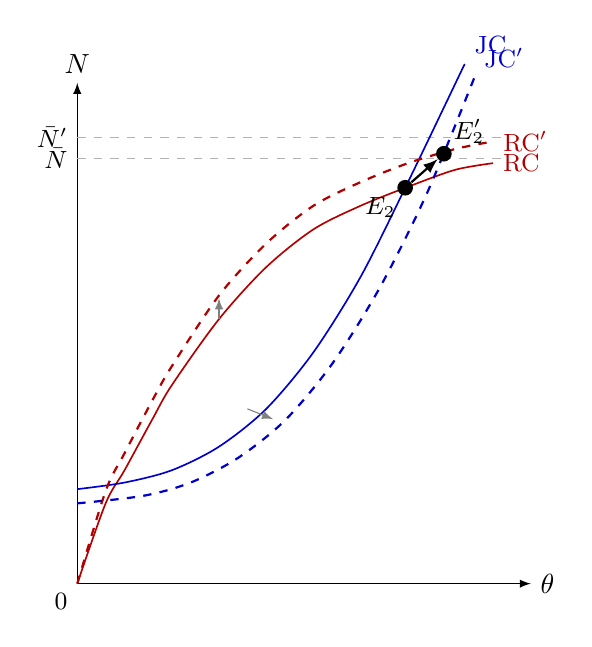
\begin{tikzpicture}[>=latex, scale=1.2,
		jc/.style={blue!80!black, semithick},
		rc/.style={red!70!black, semithick},
		jcp/.style={blue!80!black, thick, dashed},
		rcp/.style={red!70!black, thick, dashed},
		eqdot/.style={circle, fill=black, inner sep=2pt}]
		
		\draw[->] (0,0) -- (4.8,0) node[right] {$\theta$};
		\draw[->] (0,0) -- (0,5.3) node[above] {$N$};
		\node[below left, font=\small] at (0,0) {$0$};
		
		\draw[gray!60, thin, dashed] (0,4.5)
		node[left, font=\small, black] {$\bar{N}$} -- (4.5,4.5);
		\draw[gray!60, thin, dashed] (0,4.72)
		node[left, font=\small, black] {$\bar{N}'$} -- (4.5,4.72);
		
		\draw[rc] plot[smooth, tension=0.5] coordinates {
			(0,0)(0.3,0.85)(0.5,1.2)(0.8,1.75)
			(1.0,2.1)(1.5,2.8)(2.0,3.35)(2.5,3.75)
			(3.0,4.0)(3.5,4.2)(4.0,4.38)(4.4,4.45)
		} node[right, font=\small, red!70!black] {RC};
		
		\draw[jc] plot[smooth, tension=0.5] coordinates {
			(0,1.0)(0.5,1.07)(1.0,1.2)(1.5,1.45)
			(2.0,1.85)(2.5,2.45)(3.0,3.25)(3.5,4.25)(4.1,5.5)
		} node[above right, font=\small, blue!80!black] {JC};
		
		\draw[rcp] plot[smooth, tension=0.5] coordinates {
			(0,0)(0.3,0.98)(0.5,1.38)(0.8,1.95)
			(1.0,2.30)(1.5,3.05)(2.0,3.60)(2.5,4.00)
			(3.0,4.25)(3.5,4.45)(4.0,4.60)(4.4,4.68)
		} node[right, font=\small, red!70!black] {RC$'$};
		
		\draw[jcp] plot[smooth, tension=0.5] coordinates {
			(0,0.85)(0.7,0.93)(1.2,1.07)(1.7,1.33)
			(2.2,1.73)(2.7,2.33)(3.2,3.13)(3.7,4.13)(4.2,5.35)
		} node[above right, font=\small, blue!80!black] {JC$'$};
		
		\node[eqdot] at (3.47,4.19) {};
		\node[below left, font=\small] at (3.47,4.19) {$E_2$};
		
		\node[eqdot] at (3.88,4.55) {};
		\node[above right, font=\small] at (3.88,4.55) {$E_2'$};
		
		\draw[->, thick, shorten >=3pt, shorten <=3pt]
		(3.47,4.19) -- (3.88,4.55);
		
		\draw[->, gray, thin, shorten >=1pt]
		(1.8,1.85) -- (2.1,1.73);
		\draw[->, gray, thin, shorten >=1pt]
		(1.5,2.8) -- (1.5,3.05);
		
	\end{tikzpicture}
	\caption{Effect of a positive productivity shock $z\uparrow$ 
		on the steady-state equilibrium. Higher $z$ raises recruiter 
		compensation $w^{int}=\rho(N)z/\mu$, shifting the job 
		creation curve rightward (JC to JC$'$); simultaneously 
		higher income supports more product lines for given 
		employment, shifting the resource constraint curve upward 
		(RC to RC$'$, with $\bar{N}'>{\bar{N}}$). The high 
		equilibrium moves from $E_2$ to $E_2'$, with strictly 
		higher market tightness and product variety.}
	\label{fig:steady_state_curves_z}
\end{figure}

\begin{proposition}[Comparative statics]
	\label{prop:comparative_statics}
	Restricting attention to the high-$(\theta,N)$ 
	equilibrium, market tightness and product variety 
	are jointly higher under: higher productivity $z$, 
	stronger taste for variety $\zeta$, lower worker 
	bargaining power $\phi$, lower unemployment benefits 
	$b$, lower fixed entry costs $f_e$, lower exogenous 
	destruction rate $\bar{\delta}$, lower elasticity of 
	substitution $\varepsilon$, lower rate of time 
	preference $r$, and lower fixed matching cost $\kappa$. 
	Lower $\varepsilon$ and lower separation rate $\bar{s}$ 
	increase steady-state product variety $N$ but have 
	ambiguous effects on market tightness $\theta$.
\end{proposition}
	

	%%%%%%%%%%%%%%%%%%%%%%%%%%%%%%%%%%%%%%%%%
	\section{Empirical Evidence and Bartik Local Projections}\label{sec:empirical}
	%%%%%%%%%%%%%%%%%%%%%%%%%%%%%%%%%%%%%%%%%%

	\subsection{Overview and identification strategy}\label{sec:empirical_overview}

	The cross-state evidence in Section \ref{sec:introduction} establishes
	that states with structurally higher establishment exit rates accumulate
	larger unemployment gaps during recessions, but the correlation conflates
	the causal effect of exit shocks with persistent differences in industrial
	composition, institutional environment, and average firm age across
	states.  A state panel regression of labor market outcomes on local exit
	rates would confound the structural $\delta$ shock with the local demand
	conditions that drive both exits and unemployment simultaneously --- the
	classic omitted variable in any cross-sectional or within-state
	identification strategy.  The standard panel remedy of adding state and
	time fixed effects absorbs permanent cross-state heterogeneity and
	aggregate time variation but leaves untouched the within-state,
	within-time comovement between local exit activity and local business
	conditions.

	We address this using a Bartik shift-share design
	\citep{bartik_1991,goldsmith_2020}.  The instrument for state $s$ at
	quarter $t$ is a weighted average of \emph{national} industry-level
	establishment exit rates, where the weights are the state's
	pre-determined industry employment shares.  To see why this breaks the
	confound, consider Michigan in 2008: its instrument is large because
	manufacturing nationally --- not just in Michigan --- was experiencing
	a wave of permanent closings, and Michigan had a high pre-recession
	exposure to manufacturing.  The national exit rate is computed leaving
	out Michigan's own establishments (leave-one-out), so the instrument
	cannot be mechanically driven by Michigan-specific conditions.  The
	instrument thus isolates variation in exit exposure driven by a
	state's inherited industry structure interacting with national industry
	cycles, rather than by local demand or policy.

	The identifying assumption is that, conditional on state and time fixed
	effects and lagged controls, the Bartik instrument is uncorrelated with
	state-specific shocks to unemployment and vacancy creation beyond the
	exit channel. Section~\ref{sec:empirical_instr}
	describes instrument construction in detail;
	Section \ref{sec:empirical_lp} states the local projection
	specification; Section~\ref{sec:empirical_results} reports results. Section~\ref{sec:empirical_results} provides two
	validation exercises: a severity placebo that tests whether the vacancy
	IRF is driven by recession depth rather than exit exposure, and a joint
	local projection that checks robustness to controlling simultaneously
	for the layoff-and-discharge instrument.  

	\subsection{Instrument construction}\label{sec:empirical_instr}

	\paragraph{BED data and the permanence problem.}
	The underlying data source is the BLS Business Employment Dynamics
	(BED) survey, which tracks establishment-level employment via state
	unemployment insurance payroll records at quarterly frequency from
	1992Q3.  An establishment is classified as a ``closing'' in a given
	quarter if it exits the UI payroll base between consecutive March
	reference dates.  Coverage is all private-sector establishments across
	12 supersectors and all 50 states.

	Raw BED closings conflate two economically distinct events:
	\emph{permanent exits} --- establishments that dissolve irreversibly,
	destroying the associated product line and vacancy slot --- and
	\emph{temporary shutdowns}, establishments that suspend operations for
	one to three quarters before reopening.  The model's $\delta$ shock
	corresponds exclusively to permanent exit: only an irreversible
	dissolution removes a product line from the variety space and
	eliminates the recruiter's vacancy.  Using raw closings as the shock
	proxy therefore overstates the true destruction margin and introduces
	attenuation bias when the temporary-shutdown share varies over time.
	The contamination is most severe during the 2020Q2 lockdown, where
	roughly 400,000 of the recorded closings reflected government-mandated
	suspensions that subsequently reopened, but it is present at lower
	intensity throughout the sample: seasonal businesses, firms temporarily
	suspending operations during downturns, and establishments undergoing
	ownership transitions all appear as closings in BED without
	constituting permanent product-line destruction.

	\paragraph{BED Deaths as the measure of permanent exits.}
	We address this using a second BED data series that resolves the
	permanence problem directly.  In addition to closings, BED separately
	reports \emph{deaths} --- establishments absent from the UI payroll
	base for four or more consecutive quarters --- which by construction
	excludes temporary shutdowns.\footnote{BED data classes: 06 (Closings)
	records establishments absent from the next quarterly payroll file;
	08 (Deaths) records establishments absent for four or more consecutive
	quarters.  Deaths $\subseteq$ Closings in every industry$\times$quarter
	cell, so ratio is bounded above by unity by
	construction.}  Since a temporarily closed establishment re-enters the
	payroll base within one to three quarters, it never accumulates four
	consecutive absences and therefore never appears in BED Deaths.  Our
	$\delta$ instrument uses BED Deaths --- not raw closings --- as the
	numerator of the national exit rate.

	Figure~\ref{fig:bed_deaths} shows employment-weighted mean BED Closings
	and Deaths rates across 12 supersectors from 1992Q3 to 2019Q4, together
	with 10th--90th industry percentile bands.  The Deaths/Closings ratio
	(lower panel) averages 0.63 across the full sample and is remarkably
	stable over the business cycle, dipping modestly during the GFC but
	remaining well below unity throughout.  This stability implies that the
	fraction of closings that are temporary does not vary sharply over time,
	and that using Deaths directly gives a cleaner series than either raw
	closings or a time-varying permanence correction.

	\begin{figure}[h]
		\centering
		
\includegraphics[width=\linewidth]{bed_closings_vs_deaths.png}
		\caption{BED Closings and Deaths: employment-weighted rates across
		12 supersectors, 1992Q3--2019Q4.  \emph{Top panel:} mean closing
		rate (blue) and death rate (red) as percent of employment per
		quarter, with 10th--90th industry percentile bands.  Grey shading
		denotes NBER recessions.  \emph{Bottom panel:} Deaths/Closings
		ratio (dashed line at 1.0 marks the theoretical upper bound;
		ratio is bounded above by unity since Deaths $\subseteq$ Closings
		in every industry$\times$quarter cell).}
		\label{fig:bed_deaths}
	\end{figure}

	The Deaths/Closings ratio exhibits substantial cross-sector
	heterogeneity.  Mining has the lowest mean ratio (0.37), and
	Construction is similarly low (0.52), consistent with the prevalence
	of project-based and seasonal establishments that suspend operations
	temporarily without constituting permanent product-line destruction.
	Leisure and hospitality (0.58) and Other services (0.59) are also
	below the sample average.  At the other end, Manufacturing (0.71),
	Retail trade (0.70), and Information (0.70) have the highest ratios,
	reflecting structurally lower rates of temporary closure in those
	sectors.  No supersector reaches the theoretical upper bound of unity
	in any quarter of the sample.  The employment-weighted mean across all
	12 supersectors is 0.63 (2001--2019); supersector time series are
	shown in ~\ref{app:deaths_closings_supersector}.

	Most papers using BED data for shock identification
	\citep[e.g.,][]{elsby_2013} implicitly treat all
	closings as permanent.  We are not aware of a prior paper using the
	BED Deaths series to align the instrument with the structural concept
	of irreversible product-line destruction.

	\paragraph{Leave-one-out construction and base-year shares.}
	The leave-one-out (LOO) national permanent exit rate for state $s$,
	supersector $j$, quarter $t$ is
	\begin{equation}\label{eq:loo_rate}
		g^{\delta}_{-s,j,t}
		\;=\;
		\frac{\text{deaths}_{j,t}}
		     {E^{\text{nat}}_{-s,j,t_0}},
	\end{equation}
	where $E^{\text{nat}}_{-s,j,t_0}=E^{\text{nat}}_{j,t_0}-E_{s,j,t_0}$
	is base-year national employment in supersector $j$ minus state $s$'s
	own base-year employment.  The LOO correction in the denominator
	ensures that state $s$'s own exit activity cannot mechanically inflate
	its instrument value.  Numerator LOO --- subtracting state $s$'s own
	deaths from the national count --- is not implemented because
	BED state-level deaths by supersector are not publicly available.  Employment shares $\omega_{s,j}$ are drawn from the 2006
	QCEW (agglvl=54, private sector), a stable pre-GFC year that predates
	the bulk of the identifying variation.  The Bartik instrument is:
	\begin{equation}\label{eq:bartik_delta}
		B^{\delta}_{s,t}
		\;=\;
		\sum_{j} \omega_{s,j}\cdot g^{\delta}_{-s,j,t}.
	\end{equation}

	\paragraph{Residualization.}
	Raw BED exit rates co-move with industry-specific demand conditions:
	when a sector contracts nationally, establishments exit at higher rates
	\emph{and} surviving firms simultaneously reduce vacancy posting and
	raise layoffs.  An instrument built on raw $g^\delta_{j,t}$ would
	therefore partly identify the effect of industry demand contractions
	rather than the structural $\delta$ shock.  We address this by
	projecting each log shock rate on predetermined demand controls before
	Bartik aggregation, retaining the residual as the instrument input.

	The baseline residualization (v2) runs a within-industry OLS regression:
	\begin{equation}\label{eq:resid_v2}
		\log g^{\delta}_{j,t}
		\;=\;
		\alpha_j + \gamma\,\Delta\!\log p_t
		         + \lambda\,\Delta\!\log VA_{j,t-1}
		         + \nu^{\delta}_{j,t},
	\end{equation}
	where $\Delta\!\log p_t$ is aggregate nonfarm business productivity
	growth (FRED: OPHNFB) and $\Delta\!\log VA_{j,t-1}$ is real
	value-added growth in supersector $j$ lagged one quarter (BEA via
	FRED series RVAM, RVAC, etc.).  Both regressors are predetermined
	relative to the current-period shock draw: aggregate productivity is
	contemporaneous but common to all industries and thus absorbed by the
	time fixed effects in the second stage; industry VA is lagged one
	quarter to ensure strict predetermination.  The residual
	$\nu^{\delta}_{j,t}$ is then Bartik-aggregated in place of the raw
	rate, yielding $\tilde{B}^{\delta}_{s,t}$.

	The FRED BEA real value-added series begin in 2005Q1, which would
	restrict the $\delta$ residualization sample to 2005Q2.  To recover
	the full 1997Q1+ sample, we extend the quarterly VA series back to
	1992Q1 using a constrained Chow-Lin (1971) temporal disaggregation.
	An indicator regression estimated on the 2005Q1+ post-sample relates
	quarterly sectoral VA growth to real GDP growth:
	$\Delta\!\log VA_{j,t}=\alpha_j+\beta_j\,\Delta\!\log\text{GDP}_t+\varepsilon_{j,t}$.
	The pre-2005 quarterly path is recovered by applying the implied
	growth rates $\hat{\alpha}_j+\hat{\beta}_j\,\Delta\!\log\text{GDP}_t$
	recursively from the 2005Q1 anchor level.  The backcast is then
	constrained to match published BEA annual benchmarks for 1997--2004
	via a proportional Denton adjustment: for each year $A$ with annual
	benchmark $Y_{j,A}$, quarterly values are scaled by
	$Y_{j,A}/\overline{VA}_{j,A}^{\text{unconstrained}}$ so that the
	within-year average equals the published figure exactly.  Industries
	with low GDP--VA correlation (R$^2$ below threshold) receive
	$\hat{\beta}_j=0$, using only the sector-specific mean growth rate to
	avoid injecting noisy cyclical variation into the pre-period.

	After v2 residualization the cross-state correlation between the
	$\delta$ and layoffs-and-discharges (LD) Bartik instruments falls from
	approximately 0.54 on raw rates to 0.33.\footnote{As a robustness check we further augment equation~\eqref{eq:resid_v2}
		with a monetary policy sensitivity term
		$\psi(\phi_j\times\Delta MP_t)$, where $\phi_j$ is log average
		establishment size in supersector $j$ (Census CBP, 2000) and
		$\Delta MP_t$ is the quarterly change in the Wu--Xia (2016) shadow
		federal funds rate (v3 specification).  The v3 results are reported
		in Appendix~\ref{app:robustness}; v2 is the baseline throughout.}  The persistence of this residual correlation after
	controlling for industry demand cycles and aggregate productivity is
	informative: the shared variation is not a demand artifact but most
	likely reflects industry-specific financial conditions that move both
	exit rates and layoff rates simultaneously.  This motivates the joint
	local projection robustness check in
	Section~\ref{sec:empirical_results}.

	\begin{figure}[H]
		\centering
		
\includegraphics[width=\linewidth]{instrument_delta_distribution.png}
		\caption{Cross-state $\delta$ Bartik instrument distribution,
			1997Q1--2019Q4.
			\emph{Left:} residualized instrument $\tilde{B}^{\delta}_{s,t}$
			(pp of base-year employment); shading shows 25th--75th (dark) and
			10th--90th (light) cross-state percentile bands.
			\emph{Right:} z-scored cross-state means of raw (red) and
			residualized (blue dashed) instruments; $r = 0.905$.
			Orange shading (1997Q1--2000Q4): pre-LP period available for
			$\delta\to u$ but not vacancy or LD/QU.
			Grey shading: NBER recessions.}
		\label{fig:delta_distribution}
	\end{figure}

	Figure~\ref{fig:delta_distribution} documents the cross-state
	distribution of the instrument and the effect of residualization.
	Both panels extend to 1997Q1, the start of the Chow--Lin-extended
	value-added series; the orange-shaded region (1997Q1--2000Q4) marks
	the pre-JOLTS period that is available for the $\delta\to u$
	specification but not for the vacancy LP.
	The left panel shows substantial cross-sectional dispersion
	throughout, with the interquartile range widening sharply during the
	GFC.  Negative values in some states and quarters reflect
	lower-than-predicted closing rates given prevailing aggregate
	conditions and industry composition; since the local projection
	absorbs the cross-state mean via time fixed effects, identification
	comes from cross-sectional variation in residualized exposure, which
	remains well-defined regardless of sign.

	The right panel compares the z-scored cross-state means of the raw
	and residualized instruments ($r = 0.905$).  The two series track
	each other closely throughout the sample, indicating that
	residualization does not materially alter identifying variation in
	normal times.  Two episodes diverge.  During the GFC, the
	residualized mean rises somewhat more than the raw instrument at
	2008Q4 ($z = 1.51$ vs.\ $0.95$), consistent with residualization
	removing attenuating aggregate and industry-level variation.  The
	more striking divergence would appear in 2020Q2 (not shown, excluded
	from LP sample): the raw Bartik spikes to $z = 2.33$ while the
	residualized instrument falls to $z = -0.45$, because 2020Q2 BED
	closings were dominated by government-mandated temporary shutdowns
	that correlate strongly with industry composition and aggregate
	conditions; residualization correctly removes this variation, leaving
	below-average permanent destruction.  This episode illustrates
	precisely why the LP sample is capped at 2019Q4.

	The cross-state mean of the instrument exhibits a pronounced secular
	decline over the sample, falling roughly one-third from the late
	1990s to the late 2010s.  This mirrors the well-documented decline in
	aggregate labor market fluidity: the \citet{shimer_2005} quarterly
	separation rate fell proportionally over the same period, and the
	ratio of the two series is nearly constant throughout (coefficient of
	variation 14\%), indicating that permanent establishment destruction
	has declined in tandem with broader separation margins rather than
	becoming relatively more or less important over time.

	Two features of the left panel deserve note.  First, the
	cross-sectional percentile bands are narrow relative to the
	time-series movement of the mean: the within-quarter p90--p10 spread
	averages 0.045\,pp, a coefficient of variation of about 15\%.  The
	pooled standard deviation across all state-quarters ($\hat{\sigma} =
	17.4$\,pp) is therefore predominantly a time-series number, reflecting
	the common component of the instrument that moves all states together.
	The time fixed effects in the local projection absorb this common
	component; identification comes from the within-period cross-sectional
	deviations, which have a typical magnitude of roughly 0.02\,pp.
	Second, some state-quarter cells take negative values, reflecting
	lower-than-predicted closing rates given industry composition and
	aggregate conditions; these are well-defined as deviations from the
	cross-state mean and cause no identification problem.

	\subsection{Local projection specification}\label{sec:empirical_lp}

	For each horizon $h=0,1,\ldots,20$ quarters, the panel local projection
	estimating equation is
	\begin{equation}\label{eq:lp}
		y_{s,t+h} - y_{s,t-1}
		\;=\;
		\alpha_s + \alpha_t
		+ \beta_h\,\tilde{B}^{\delta}_{s,t}
		+ \gamma_1\,y_{s,t-1}
		+ \gamma_2\,\log L_{s,t-1}
		+ \varepsilon_{s,t+h},
	\end{equation}
	where $y_{s,t}$ is the labor market outcome of interest for state $s$ in quarter $t$,
	$\tilde{B}^{\delta}_{s,t}$ is the residualized $\delta$ Bartik instrument
	constructed in Section~\ref{sec:empirical_instr}, $\alpha_s$ and
	$\alpha_t$ are state and time fixed effects, $y_{s,t-1}$ is the lagged
	outcome, and $L_{s,t-1}$ is the lagged labor force.  The left-hand side
	measures the cumulative $h$-period change relative to the quarter before
	the shock, so the sequence $\{\hat\beta_h\}$ traces the impulse response
	directly.  Standard errors are clustered at the state level ($n=50$).

	The two outcomes are the state unemployment rate $u_{s,t}$ and vacancy
	rate $v_{s,t}$, both in percentage points (unemployed persons or
	vacancies as a share of the labor force).  Concretely,
	$v_{s,t} = 100 \times V_{s,t}/L_{s,t}$, where $V_{s,t}$ is the
	quarterly average of monthly JOLTS job-openings stocks (seasonally
	adjusted) and $L_{s,t}$ is the LAUS labor force.  The two
	specifications differ only in the autoregressive control $y_{s,t-1}$.

	The estimation sample runs from 2001Q1, when JOLTS state vacancy data
	become available, through 2019Q4; observations with $t+h >
	\text{2019Q4}$ are dropped to exclude COVID-19.\footnote{The $\delta$
		unemployment equation can be estimated back to 1997Q1 using the
		Barnichon (2010) Composite Help-Wanted Index as a pre-JOLTS vacancy
		proxy; extending the sample attenuates the IRF modestly (peak
		$+1.07$ pp vs.\ $+1.50$ pp) because the 1997--2000 expansion years
		exhibit faster reabsorption of displaced workers.  We use the 2001Q1
		baseline throughout to maintain a common sample across both outcomes.}
	The instrument $\tilde{B}^{\delta}_{s,t}$ has cross-sectional standard
	deviation $\hat\sigma_{\tilde{B}^\delta} = 17.4$ pp; all reported
	$\hat\beta_h$ are scaled by $\hat\sigma_{\tilde{B}^\delta}^{-1}$ so
	that the impulse responses correspond to a one-standard-deviation shock.

	We also construct Bartik instruments for layoffs-and-discharges
	$\tilde{B}^{\text{LD}}$ (JOLTS LD) and quits $\tilde{B}^{\text{QU}}$
	(JOLTS quits), using the same 2006 QCEW base-year shares and v2
	residualization.  Neither is treated as a well-identified separate
	estimation target.  $\tilde{B}^{\text{LD}}$ conflates genuine match
	dissolution at surviving establishments with vacancy withdrawals at
	partially closing firms, mixing $s$- and $\delta$-type events in
	proportions that vary across industries and cycles; moreover,
	$\tilde{B}^{\delta}$ Granger-causes future LD through $h=12$ while the
	reverse predictability fades by $h=8$, indicating that LD is partly
	endogenous to destruction.  $\tilde{B}^{\text{QU}}$ is procyclical and
	driven largely by job-to-job transitions, which represent a worker gain
	for one employer offset by a hire at another and have no clear mapping
	to the model's match separation shock $s$; we include it as a diagnostic
	instrument only.\footnote{In particular, a high quit rate in an industry
	does not imply that vacancies go unfilled --- the quitting worker is
	typically replaced by a job-to-job mover from elsewhere, so the net
	effect on aggregate vacancies is near zero.  This is conceptually
	distinct from the $s$ shock in the model, which destroys a match and
	triggers a vacancy repost.}  Both instruments and their local
	projections are reported in \ref{app:diagnostics}.

	\begin{figure}[H]
		\centering
		
\includegraphics[width=0.92\textwidth]{lp_irf_delta_uv_baseline.png}
		\caption{Impulse responses of the state unemployment rate (left)
			and vacancy rate (right) to a one-standard-deviation increase
			in the residualised $\delta$ Bartik instrument
			($\hat{\sigma}_{\tilde{B}^\delta}=17.4$ pp, 2001Q1--2019Q4).
			Both outcomes are estimated from panel local projections with
			state and time fixed effects; standard errors are clustered at the
			state level ($n=50$).  Shaded band: 90\% confidence interval;
			dashed lines: 95\% confidence interval.  The instrument is
			BED establishment deaths (equation~\eqref{eq:bartik_delta}),
			residualized on aggregate productivity growth and lagged industry
			value-added growth (equation~\eqref{eq:resid_v2})}
		\label{fig:delta_uv_irf}
	\end{figure}

	\subsection{Results}\label{sec:empirical_results}

	% --- delta -> u and delta -> v IRFs ---

	Figure~\ref{fig:delta_uv_irf} reports the impulse responses of the
	state unemployment rate and vacancy rate to a one-standard-deviation
	increase in the residualized $\delta$ Bartik instrument
	($\hat{\sigma}_{\tilde{B}^\delta} = 17.4$ pp, 2001Q1--2019Q4 sample).
	The unemployment response rises steadily from $0.22$ pp at $h=0$ to
	a plateau of $+1.71$ pp by $h=17$--$20$, remaining highly significant
	throughout ($p < 0.001$ from $h=0$).  The vacancy response falls
	persistently from $-0.11$ pp at $h=0$ to a trough of $-0.58$ pp at
	$h=18$, significant at $p < 0.01$ from $h=2$ onward and remaining so
	through $h=20$.  The simultaneous and persistent rise in unemployment
	alongside the fall in vacancies traces the outward leg of a Beveridge
	loop, consistent with the model's central prediction that permanent
	product-line destruction depletes the vacancy stock rather than merely
	suspending it.

	A notable feature of the two IRFs is their asymmetric dynamics at
	medium horizons: the vacancy response stabilizes around $h = 12$--$14$
	while the unemployment response continues to rise through $h = 20$.
	This pattern is consistent with a recovery path in which new vacancy
	creation resumes before the unemployment pool fully clears.  Whether the
	calibrated model replicates this relative timing is testable and will
	be assessed in Section~\ref{sec:quantitative}.

	% --- Severity placebo ---

	A natural concern is that the $\delta$ Bartik instrument may inadvertently
	capture recession severity: states with structurally high establishment turnover
	may also experience worse aggregate downturns, so the IRF could reflect
	demand-driven labor-market deterioration rather than product-line destruction
	per se.  We address this with a severity placebo that augments the baseline
	local projection with two interactions: $\tilde{B}_t^\delta \times
	\bar{u}_t^{\text{nat}}$, a level proxy for underlying economic slack, and
	$\tilde{B}_t^\delta \times \Delta\bar{u}_t^{\text{nat}}$, a flow proxy for
	cyclical momentum.  If the instrument were a severity proxy, these interactions
	should absorb the baseline IRF.  Instead, both interaction coefficients are
	insignificant at every horizon $h = 0, \ldots, 20$ for the vacancy outcome, and
	the baseline $\delta \to v$ coefficients are unchanged in magnitude and
	significance.  This is the cleanest external validity check in the paper: the
	vacancy response to establishment destruction is not explained by where
	the aggregate economy happens to stand in the cycle.  The severity placebo
	also passes for the unemployment outcome, though the interpretation is less
	sharp given the natural correlation between any adverse state-level shock and
	local unemployment.  Robustness results for the alternative instruments and
	the joint local projection are collected in
\ref{app:diagnostics}.

	%%%%%%%%%%%%%%%%%%%%%%%%%%%%%%%%%%%%%%%%%%
	\section{Quantitative analysis}\label{sec:quantitative}
	\subsection{Relationship to Coles and Kelishomi}\label{sec:ck_comparison}

	\citet{coles_2018} establish the mechanism at the heart of our framework: sunk
	vacancy creation costs and a destruction shock that simultaneously eliminates
	filled jobs and posted vacancies can replicate both the volatility and the
	Beveridge-curve dynamics of the U.S.\ labor market. Because each filled job and
	each vacancy corresponds to an active product line, their shock is structurally
	equivalent to the $\delta$ shock in our model. Finitely elastic vacancy creation
	limits the speed at which new product lines are opened following a destruction
	event, so the vacancy stock and unemployment comove negatively---consistent with
	the data.

	Two features of their calibration require revisiting. First, \citet{coles_2018}
	set $\delta = 0.031$ per month, effectively treating all aggregate separations as
	product destruction. BLS Business Employment Dynamics data place the
	employment-weighted permanent exit rate at $\bar\delta \approx 1.1\%$ per
	quarter, roughly one-ninth of the aggregate separation rate $\bar\tau = 9.3\%$
	per quarter; their calibration therefore overstates the destruction margin by an
	order of magnitude. \citet{gabrovski_2025} show that once $\delta$ and the match
	separation rate $s$ are distinguished and $\delta$ is calibrated to establishment
	exit data, the unconditional correlation between unemployment and labor
	productivity---notoriously difficult to match in Diamond--Mortensen--Pissarides
	models---attenuates toward its empirical value. Second, CK do not model
	endogenous firm entry, so their framework is silent on business formation
	dynamics and the variety channel through which entry costs propagate aggregate
	shocks.

	Our model addresses both gaps. We retain CK's sunk-cost structure and extend it
	to include endogenous entry and exit, imperfect competition, and a product-variety
	externality. We calibrate $\delta$ directly to BED Deaths data and separately
	identify $s$ from total separations via the \citet{shimer_2012} decomposition.
	The estimation correspondingly expands the moment set to include the permanent
	exit rate and business applications, and supplements unconditional moments with
	identified impulse responses from the Bartik local projections to separately pin
	down the propagation dynamics of $\delta$ and $s$ shocks.

	\subsection{Calibration and estimation}\label{sec:calib}

	This section sets out our estimation and calibration strategy, the taxonomy of
	parameters, and the explicit mapping from empirical targets to model objects.

	\medskip\noindent\textbf{Estimation framework.}
	We estimate the model by Bayesian simulated method of moments, combining two
	complementary sets of moment conditions that together over-identify the parameter
	vector.

	The first set consists of unconditional second moments of HP-filtered aggregate
	time series, extending \citet{coles_2018}. We target three groups: (i)~standard
	deviations ($m_1$), (ii)~contemporaneous pairwise correlations ($m_2$), and
	(iii)~first-order autocorrelations ($m_3$) for unemployment, vacancies,
	separations, the job-finding rate, the permanent exit rate, business
	applications, and labor productivity. The full empirical moment matrix is
	reported in Table~\ref{tab:smm_moments}. All series are log-transformed and
	HP-filtered with smoothing parameter $\lambda = 100{,}000$ before computing
	moments; the identical filter is applied to simulated model data when evaluating
	$m(\theta)$. This symmetric treatment renders HP-filtered second moments a valid
	indirect inference target: \citet{canova_ferroni_2011} establish that applying
	the same filter to data and simulated output controls for any filter-induced
	distortion, even when the filter introduces spurious dynamics in isolation.


\begin{table}[htbp]
\centering
\begin{threeparttable}
\caption{Business Cycle Moments}
\label{tab:smm_moments}
\begin{tabular}{l r @{\hspace{6pt}\vline\hspace{6pt}} r r r r r r r @{\hspace{6pt}\vline\hspace{6pt}} r}
\toprule
  &  $\sigma(x)$  &  \multicolumn{7}{c}{Contemporaneous correlations}  &  $\rho_1(x)$  \\
\cmidrule(lr){3-9}
  &  &  $u$  &  $v$  &  $s$  &  $f$  &  $\delta$  &  $a$  &  $z$  &  \\
\midrule
  Unemployment  &  0.2148  &  $1$  &    &    &    &    &    &    &  0.894  \\
  Vacancies  &  0.2009  &  -0.826  &  $1$  &    &    &    &    &    &  0.945  \\
  Separations  &  0.1164  &  0.513  &  -0.435  &  $1$  &    &    &    &    &  0.422  \\
  Job-finding rate  &  0.1473  &  -0.865  &  0.674  &  -0.037  &  $1$  &    &    &    &  0.910  \\
  Exit rate  &  0.0998  &  -0.041  &  0.127  &  0.492  &  0.359  &  $1$  &    &    &  0.436  \\
  Business applications  &  0.1264  &  -0.335  &  0.541  &  -0.227  &  0.250  &  -0.192  &  $1$  &    &  0.813  \\
  Labor productivity  &  0.0191  &  -0.139  &  0.299  &  -0.125  &  0.035  &  -0.158  &  0.404  &  $1$  &  0.890  \\
\midrule
  \multicolumn{10}{l}{\textit{Derived statistics}}  \\
  \quad $\sigma(\theta)/\sigma(z)$  &  20.83  &    &    &    &    &    &    &    &    \\
\bottomrule
\end{tabular}
\begin{tablenotes}[flushleft]
\footnotesize
\item \textit{Note:} HP filter with $\lambda = 100{,}000$ applied to log-levels of each series. Correlations use pairwise-complete observations; the shortest series (business applications, $a$) begins 2004Q3. Sources --- $u$: BLS LAUS; $v$: Barnichon (2010) composite HWI spliced with BLS JOLTS at 2001Q1; $s$, $f$: Shimer (2012) continuous-time flows from CPS; $\delta$: BLS BED Deaths (dataclass 08), employment-weighted; $a$: BFS high-propensity business applications (BAWBATOTALSAUS) per capita; $z$: BLS PRS85006163 (output per hour, nonfarm business).
\end{tablenotes}
\end{threeparttable}
\end{table}
	The second set consists of empirically identified impulse responses from the
	Bartik local projections of Section~\ref{sec:empirical}: the $h=0,\ldots,H$
	quarter paths of unemployment and vacancies following a one-standard-deviation
	$\delta$ shock. Following \citet{christiano_2016}, we form a Gaussian
	quasi-likelihood based on the sampling distribution of the LP estimator:
	\begin{align}\label{eq:ql_irf}
		\log \mathcal{L}_{\mathrm{IRF}}(\theta)
		= -\tfrac{1}{2}(\hat\beta - \beta(\theta))'\Omega_\beta^{-1}(\hat\beta -
		\beta(\theta)),
	\end{align}
	where $\hat\beta$ stacks the two estimated IRF paths, $\beta(\theta)$ is the
	corresponding model-implied path computed from the linearized state-space
	representation, and $\Omega_\beta$ is the sampling covariance estimated by wild
	cluster bootstrap with $n=50$ state clusters. Unlike a full structural
	likelihood, this quasi-likelihood conditions on the reduced-form LP estimator
	rather than integrating over the model's DGP; it is valid precisely because the
	Bartik design yields consistent, approximately normal IRF estimates without
	requiring distributional assumptions on the structural shocks beyond the LP
	moment conditions of Section~\ref{sec:empirical_lp}.

	A filtering asymmetry between the two blocks is present by design: unconditional
	moments are statistics of HP-filtered data, while IRF coefficients are estimated
	from level regressions. This is resolved on the model side. Model moments
	$m(\theta)$ are computed from simulated-then-filtered data, mirroring the data
	construction. Model IRFs $\beta(\theta)$ are read directly from the state-space
	impulse response without filtering, mirroring the LP estimation. The two objects
	therefore target genuinely distinct features of the model---cyclical second-moment
	structure and shock-specific propagation dynamics---in a way that is internally
	consistent on both the data and model sides.

	The two blocks provide complementary identification. Unconditional moments
	discipline the level and cyclical volatility of the destruction and separation
	processes, the amplification and comovement structure, and the persistence of key
	aggregates. The IRF block separately identifies the dynamic transmission of
	$\delta$ shocks---in particular, the simultaneous elimination of vacancies that
	distinguishes $\delta$ from $s$ and generates persistent Beveridge-curve
	dislocations---identification unavailable from unconditional moments alone, which
	conflate the contributions of all three shocks.

	To prevent the IRF block from mechanically dominating the joint objective by
	virtue of moment count, we normalize each block's quadratic form by its
	dimension. Letting $K_\beta$ denote the number of IRF moment conditions and
	$K_m$ the number of unconditional moments, the log-posterior kernel is
	\begin{align}\label{eq:posterior}
		\log p(\theta \mid \mathrm{data})
		\propto \log\pi(\theta)
		- \frac{1}{2K_\beta}(\hat\beta - \beta(\theta))'\Omega_\beta^{-1}
		(\hat\beta - \beta(\theta))
		- \frac{1}{2K_m}(\hat m - m(\theta))'\Omega_m^{-1}(\hat m - m(\theta)),
	\end{align}
	where $\hat m$ collects the empirical moments from Table~\ref{tab:smm_moments},
	$m(\theta)$ the corresponding model-implied moments from simulated HP-filtered
	data, and $\Omega_m$ a HAC covariance estimated by block bootstrap with block
	length eight quarters. The degrees-of-freedom normalization ensures each block
	contributes equally in expectation when the model is correctly specified, since
	each quadratic form is approximately $\chi^2(K)$ with expectation $K$ under the
	null \citep{dridi_2007}. Appendix~\ref{app:weighting_robustness} reports
	robustness to rescaling the unconditional moment block by factors of one-half and
	two.

	\medskip\noindent\textbf{Parameter taxonomy.}
	We partition the full parameter space $\Theta$ into three blocks.
	
	\emph{Estimated block} $\Theta_e$: structural parameters and shock processes
	whose identification comes from business-cycle moments. This block contains the
	replacement value $b$; the sunk-cost share $x_v$ of total recruiting expenditure
	(which maps to the fixed matching cost $\kappa$ in Stage~4 below); the inverse
	elasticity of entry with respect to vacancy value $\xi^{-1}$; the endogenous
	exit share $\omega_\delta \equiv (1-F(x^c))/\delta_e$; the inverse
	intertemporal elasticity of substitution $\sigma$; and the persistence
	$\rho_x$ and conditional standard deviation $\sigma_x$ of each shock
	$x\in\{z,\delta,s\}$.
	
	\emph{External block}: parameters set directly from microeconomic evidence or
	long-run data. We fix the annual discount rate $r=4\%$ and the matching-function
	elasticity $\eta_L=0.6$. Following \citet{jaimovich_2008}, 21\% of job
	destruction is attributable to establishment exit; combined with an aggregate
	monthly separation rate of $\tau=3.1\%$, this implies a monthly destruction
	rate $\delta_e=0.651\%$ (annual: $7.54\%$). We set the elasticity of
	substitution $\varepsilon=4.3$, implying a gross markup $\mu=\varepsilon/(\varepsilon-1)\approx1.30$.
	
	\emph{Dependent block} $\Theta_d$: parameters implied jointly by the
	normalizations, the external block, and a draw from $\Theta_e$ via the
	four-stage calibration procedure described below. We normalize the steady-state
	mass of firms $N=1$ and the wage $w=1$. The remaining parameters—$z$, $\phi$,
	$f_e$, $A$, $s$, $\psi$, $f_m$, $x_m$, $\kappa$, $\delta$—are recovered from
	the following targets:
	
	\begin{center}
		\ra{1.3}
		\begin{tabular}{lll}
			\toprule
			Target & Value & Parameter(s) identified \\
			\midrule
			Annual product destruction rate $\delta_e^{ann}$  & $7.54\%$  &
			Monthly $\delta_e$, exogenous rate $\delta=(1-\omega_\delta)\delta_e$ \\
			Endogenous exit share $\omega_\delta$  & estimated  &
			Exogenous rate $\delta$, separation rate $s$ \\
			Job-finding rate $f^{emp}$  & $41\%$      &
			Destruction-adjusted rate $f$, tightness $\theta$, level $A$ \\
			Vacancy-filling rate $q^{emp}$  & $80\%$  &
			Destruction-adjusted rate $q$, tightness $\theta$ \\
			Aggregate separation rate $\tau$   & $3.1\%$    &
			Match separation rate $s=(\tau-\delta_e)/(1-\delta_e)$ \\
			Recruiting cost share $X/Y$         & $1.5\%$    &
			Vacancy value $Q$, then $\kappa$, $z$, $f_e$, $x_m$, $\phi$ \\
			Fixed cost share $X^c/Y$            & $10\%$  &
			Within-sector ratio $X^c/Y^c$, profit share $\pi_s$ \\
			Wage normalization $w=1$            & ---       &  Productivity $z$ \\
			Firm-mass normalization $N=1$       & ---       &  Entry cost $f_e$ \\
			\bottomrule
		\end{tabular}
	\end{center}
	
	\medskip\noindent\textbf{Calibration algorithm.}
	Given a draw from $\Theta_e$ and the external block, we recover $\Theta_d$ in
	four sequential stages.
	
	\medskip\noindent\textit{Stage 1: direct conversions (targets $\to$ fundamentals).}
	The destruction rate target $\delta_e^{ann}$ and endogenous share $\omega_\delta$
	pin
	\begin{align}
		\delta_e = 1-(1-\delta_e^{ann})^{1/12}, \qquad
		\delta   = (1-\omega_\delta)\,\delta_e.
	\end{align}
	The match separation rate follows from the aggregate target:
	\begin{align}
		s = \frac{\tau - \delta_e}{1-\delta_e}.
	\end{align}
	The empirical job-finding and vacancy-filling rates are corrected for destruction
	before use: $f=f^{emp}/(1-\delta_e)$, $q=q^{emp}/(1-\delta_e)$.
	Market tightness $\theta=f/q$, the unemployment rate
	$u=\tau/(\tau+(1-\delta_e)f)$, and the matching-function level parameter
	$A=f/\theta^{1-\eta_L}$ are then computed analytically.
	
	\medskip\noindent\textit{Stage 2: profit share (root-find $X^c/Y^c$).}
	The fixed-cost share of retail output $X^c/Y^c$ is not directly observed; we
	recover it by solving
	\begin{align}\label{eq:calib_stage2}
		\frac{X^c/Y}{(Y^c/Y^{Gross})(Y^{Gross}/Y)} = \frac{X^c}{Y^c},
	\end{align}
	where $Y^c/Y^{Gross}=(r+\delta_e)/(r+\delta_e+\delta_e\pi_s)$ and
	$Y^{Gross}/Y=1+X/Y+X^c/Y$. The profit share $\pi_s=1/\varepsilon - X^c/Y^c$
	is a residual: retail value added equals the Lerner markup $1/\varepsilon$
	after paying stochastic fixed costs.
	
	\medskip\noindent\textit{Stage 3: cost-distribution parameters (root-find $\psi$).}
	Given $\pi_s$, we recover the mass fraction of continuing cost draws,
	$\mathit{cons}$, from
	\begin{align}\label{eq:calib_stage3}
		\pi_s = \frac{\mu-1}{\mu}\,(1-\mathit{cons})\,
		\frac{r+\delta_e}{r+\delta_e+\mathit{cons}\,(1-\delta_e)},
	\end{align}
	then map $\mathit{cons}$ to the power-law shape parameter
	$\psi = (\mathit{cons}/p_0)\,/\,(1-\mathit{cons}/p_0)$
	and location parameter $f_m = x^c/\zeta^{1/\psi}$, where
	$\zeta=([(1-\delta_e)/(1-\delta)]-(1-p_0))/p_0$ is the quantile of the exit
	threshold within the continuous part of the cost distribution. Here $p_0=0.5$
	is fixed externally as the probability that the continuation cost is positive.
	
	\medskip\noindent\textit{Stage 4: vacancy value (root-find $Q$).}
	We solve for the steady-state vacancy value $Q$ by requiring the recruiting-cost
	share to equal its target: $X/Y = 1.5\%$. Given a trial value $Q$, the
	contact-rate value $K=(r+\delta_e)Q/(1+r)$ and the fixed matching cost
	$\kappa=(1-x_v)/x_v \cdot K/q$ follow from the sunk-cost split $x_v$. Total
	recruiting expenditure $X=e/(1+\xi^{-1})\cdot Q+\kappa qv$, the interior
	wage $w^{int}$, and firm-level output $Y^c=\rho z L^c$ are computed
	sequentially. The value of $Q$ is chosen so that output implied by the
	recruiting-cost target, $Y=X/(X/Y)$, coincides with expenditure-side
	output $Y=C+\nu^f N^e$.
	The remaining dependent parameters are then recovered analytically:
	\begin{align}
		z      &= (\mu/\rho)\,w^{int}, \label{eq:z_calib}\\
		f_e    &= \pi_s\, z\, L^c\,(1-\delta_e)\,\mu\,/\,(N\,(r+\delta_e)), \label{eq:fe_calib}\\
		\phi   &= \frac{w-b}{w^{int}-K+\theta(K+q\kappa)-b}, \label{eq:phi_calib}\\
		x_m    &= Q\,/\,e^{\xi^{-1}}. \label{eq:xm_calib}
	\end{align}
	The normalizations provide clean intuition: $w=1$ pins $z$ via
	\eqref{eq:z_calib} because the interior wage $w^{int}=\rho z/\mu$ is
	proportional to productivity; $N=1$ pins $f_e$ via \eqref{eq:fe_calib}
	because free entry ties the mass of product lines to the entry cost; and the
	recruiting-cost share target $X/Y=1.5\%$, once $Q$ is found, pins bargaining
	power $\phi$ via \eqref{eq:phi_calib}.
	
	\medskip\noindent\textbf{Discussion of $b$ and $\phi$.}
	In our labor market framework, the labor share and the search wedge $w/w^{int}$
	both depend on Nash bargaining power $\phi$ and the worker outside option $b$.
	\citet{shimer_2005} interprets $b$ as unemployment insurance and calibrates it
	to $0.4$, finding that technology shocks generate an order-of-magnitude too
	little unemployment and vacancy volatility, attributing this to excessively
	wage-elastic labor markets. \citet{hagedorn_2008} show that even adjusting $\phi$
	to match the mild empirical wage cyclicality leaves tightness volatility
	unchanged; what matters is the proportional response of profits to productivity.
	We resolve this debate by estimating $b$ via simulated method of moments and, given the draw
	of $b$, selecting $\phi$ internally to satisfy~\eqref{eq:phi_calib}—ensuring
	that the wage normalization and labor-share implications are mutually consistent.
	Our model links market power with search frictions, making the labor share a
	natural discipline on both $\phi$ and $b$. Matching the consumption share and
	labor share jointly also implies a realistic stock-market capitalization-to-output
	ratio without sacrificing fit on business-cycle moments.
	
	
	
	\subsection{Posterior estimates}
	% Include posterior-prior plots
	% Include table of estimates
	% Include moments generated at posterior mean
	\subsection{Impulse responses}
	% Describe transmission mechanism of impulse responses
	\subsection{Inspecting the mechanism}
	We begin by emphasizing the significance of variety effects by comparing the impulse responses of our model with those of a similar model where $\zeta=0$. Importantly, both versions maintain consistent markup, labor share of income, and other calibrated targets. As illustrated in Figure\ref{fig:variety_effects_irf_z_comparison}, we observe that unemployment exhibits increased persistence, which is closely linked to changes in business formation and the corresponding measure of product lines. Given that the number of firms, and consequently the relative price $p$, is predetermined, the immediate response of unemployment remains unaffected by variety effects.
	\begin{figure}[H]
		\includegraphics[width=\textwidth]{"variety_effects_irf_z_comparison"}
		\centering
		\caption{}
		\label{fig:variety_effects_irf_z_comparison}
	\end{figure}
	Second, we investigate the impact of risk aversion by comparing the effects of a destruction shock in our baseline model to those in a risk-neutral environment, typical of the benchmark search model, as depicted in Figure \ref{fig:risk_aversion_comparison_delta_shock}. Our primary finding is that labor market variables are generally insensitive to the consumption smoothing motive. This result arises from two factors: (1) the finite elasticity of vacancy creation inherently encourages smoothing of vacancy creation, and (2) new vacancies constitute a small portion of the overall vacancy stock. However, with either more elastic vacancy creation or increased product destruction, the responses of vacancies and unemployment would differ. Notably, risk aversion significantly influences the responses of business formation, consumption, and output. In the absence of convex adjustment costs in business formation, a persistent destruction shock substantially diminishes the present discounted value of profits under risk neutrality. Essentially, the incentive to initiate a new product line declines with a persistent destruction shock, leading households to favor scaling back business formation and increasing consumption instead. In a risk-neutral scenario, a destruction shock would prompt consumption and output to rise alongside unemployment, thereby limiting their role in driving business cycle dynamics. Therefore, when considering the dynamics of business formation—key macroeconomic aggregates—the degree of risk aversion becomes crucial.
	\begin{figure}[H]
		\includegraphics[width=\textwidth]{"risk_aversion_comparison_delta_shock"}
		\centering
		\caption{}
		\label{fig:risk_aversion_comparison_delta_shock}
	\end{figure}
	
	Third, we explore the impact of the inverse elasticity of vacancy creation $\xi^{-1}$. Specifically, we compare the baseline response to the model recalibrated with $\xi^{-1}=0.5$.  In this analysis, we focus on the responses to both technology and destruction shocks, noting significant differences between the two scenarios.
	
	Figure \ref{fig:elastic_comparison_delta_shock} illustrates the responses under a destruction shock. With increased elasticity in vacancy creation, the number of new vacancies rises, which mitigates the increase in unemployment. This effect also leads to a smaller decline in business formation and output. Importantly, despite the heightened elasticity in entry, the negative correlation between unemployment and vacancies persists, maintaining the integrity of the Beveridge curve.
	\begin{figure}[H]
		\includegraphics[width=\textwidth]{"elastic_comparison_delta_shock"}
		\centering
		\caption{}
		\label{fig:elastic_comparison_delta_shock}
	\end{figure}
	
	Figure \ref{fig:elastic_comparison_tech_shock} depicts the responses to a contractionary technology shock. With more elastic vacancy creation, the number of new vacancies declines significantly, leading to a substantial reduction in the overall vacancy stock and, consequently, a pronounced increase in unemployment. However, the responses of business formation, consumption, and output remain relatively unchanged. Thus, increased elasticity in vacancy creation amplifies the impact of technology shocks while diminishing the effects of destruction shocks. In other words, incorporating finitely elastic vacancy creation into the benchmark search model allows destruction shocks to have a more pronounced effect on unemployment, while reducing the influence of technology shocks.
	\begin{figure}[H]
		\includegraphics[width=\textwidth]{"elastic_comparison_tech_shock"}
		\centering
		\caption{}
		\label{fig:elastic_comparison_tech_shock}
	\end{figure}
	
	\citet{pissarides_2009} proposes fixed matching costs as a means to make average hiring costs less cyclical, so that job creation becomes more sensitive to fluctuations in technology. This logic applies in our model as well, so we omit the impulse responses. However, Figure \ref{fig:kappa_comparison_delta_shock} shows that the responses are nearly identical in the case of a destruction shock.
	\begin{figure}[H]
		\includegraphics[width=\textwidth]{"kappa_comparison_delta_shock"}
		\centering
		\caption{}
		\label{fig:kappa_comparison_delta_shock}
	\end{figure}
	\textcolor{red}{To do: include plot for corresponding BGM model}
	Finally, we compare a technology shock in this framework to \citet{bilbiie_2012}. There are several key differences. First, labor reponds only via the extensive margin. It is predetermined on impact and can only expand gradually. A Frisch elasticity of labor supply of one produces a similar response of output on impact. 
	%%%%%%%%%%%%%%%%%%%%%%%%%%%%%%%%%
	\section{Conclusion}\label{ref:conclusion}
	\newpage
	\appendix

	%%%%%%%%%%%%%%%%%%%%%%%%%%%%%%%%%%%%%%%%%%
	\section{Data sources}\label{app:data_sources}

	\begin{table}[H]
	\centering\footnotesize
	\caption{Data sources\label{tab:data_sources}}
	\begin{tabular}{@{}p{3.8cm}p{2.4cm}p{4.2cm}p{3.2cm}@{}}
		\toprule
		Series & Source & Frequency \& coverage & Unit \\
		\midrule
		\multicolumn{4}{l}{\textit{Panel A: Instrument construction}} \\[2pt]
		BED establishment deaths (dc~08) & BLS BED   & Quarterly, 1992Q3--2024Q2  & National $\times$ supersector \\[2pt]
		QCEW employment shares           & BLS QCEW  & Annual, base year 2006     & State $\times$ supersector    \\[2pt]
		Layoffs \& discharges (LD)        & BLS JOLTS & Monthly, 2001Q1--2023Q1    & National $\times$ supersector \\[2pt]
		Quits (QU)                       & BLS JOLTS & Monthly, 2001Q1--2023Q1    & National $\times$ supersector \\[5pt]
		\multicolumn{4}{l}{\textit{Panel B: Residualization controls}} \\[2pt]
		Labor productivity (OPHNFB)      & BLS, FRED & Quarterly, 1947Q1--present & National                      \\[2pt]
		Value added by industry          & BEA, FRED & Quarterly, 2005Q1--present & National $\times$ supersector \\[5pt]
		\multicolumn{4}{l}{\textit{Panel C: LP outcome variables}} \\[2pt]
		Unemployment rate                & BLS LAUS  & Monthly, 1990M1--present   & State                         \\[2pt]
		Civilian labor force             & BLS LAUS  & Monthly, 1990M1--present   & State, thousands              \\[2pt]
		Job openings                     & BLS JOLTS & Monthly, 2001M1--present   & State, thousands              \\[5pt]
		\multicolumn{4}{l}{\textit{Panel D: Bayesian estimation moments}} \\[2pt]
		Job-finding rate ($f_t$)         & BLS CPS   & Monthly, 1948M1--present   & National                      \\[2pt]
		Separation rate ($s_t$)          & BLS CPS   & Monthly, 1967M1--present   & National                      \\[2pt]
		Business formations (BF8)        & Census BFS & Quarterly, 2004Q3--present & National                     \\[2pt]
		\bottomrule
	\end{tabular}
	\end{table}

	\noindent Panel~A instruments are constructed as Bartik shift-share aggregates.
	BED deaths (dataclass~08) counts employment at establishments absent for four or more consecutive quarters, excluding temporary shutdowns by construction.
	QCEW shares are fixed at the 2006 base year and leave-one-out corrected.
	LD and QU are summed from monthly to quarterly; QU serves as a placebo instrument (Appendix~\ref{app:qu_placebo}).
	Panel~B controls enter the v2 residualization as first log-differences: aggregate productivity growth (OPHNFB) and lagged industry value-added growth (12 BEA supersector series via FRED: VAPGDPIP, VAMFNIP, VACONIP, VATRDIP, VATRIIP, VAINIP, VAFNSIP, VAPBSIP, VAEDUHIP, VALAHIP, VAOSIP, VAGOSIP); the value-added series are extended to 2001Q1 via Chow--Lin temporal disaggregation using BLS employment as the indicator.
	Panel~C outcomes are averaged from monthly to quarterly; the vacancy rate is defined as job openings divided by civilian labor force, expressed in percentage points.
	Panel~D moments are national aggregates used as targets in Bayesian estimation.
	Job-finding and separation rates are constructed from CPS unemployment flows with the continuous-time correction for time-aggregation bias \citep{shimer_2005}.
	BF8 counts business applications with planned wages that appear in QCEW within eight quarters, and proxies for the model entry flow $N^e_t$.


	%%%%%%%%%%%%%%%%%%%%%%%%%%%%%%%%%%%%%%%%%%
	\section{Instrument diagnostics and robustness}\label{app:diagnostics}
	\subsection{Deaths/Closings ratio by supersector}\label{app:deaths_closings_supersector}
	Figure~\ref{fig:deaths_by_supersector} plots the Deaths/Closings ratio
	for each of the 12 BLS supersectors separately, divided into the six
	with the highest mean ratio (left panel) and the six with the lowest
	(right panel).  Across all sectors and quarters the ratio remains
	strictly below unity, confirming that BED Deaths are always a subset
	of BED Closings.  The cross-sector range is wide: Manufacturing,
	Retail, and Information cluster near 0.70, while Mining (0.37) and
	Construction (0.52) are substantially lower, consistent with the
	prevalence of project-based and cyclically suspended establishments in
	those sectors.  The ratio is broadly stable within each supersector
	over time, with no systematic cyclical pattern, supporting the use of
	a fixed Deaths/Closings fraction as the implicit permanence assumption
	in our instrument.
	
	\begin{figure}[H]
		\centering
		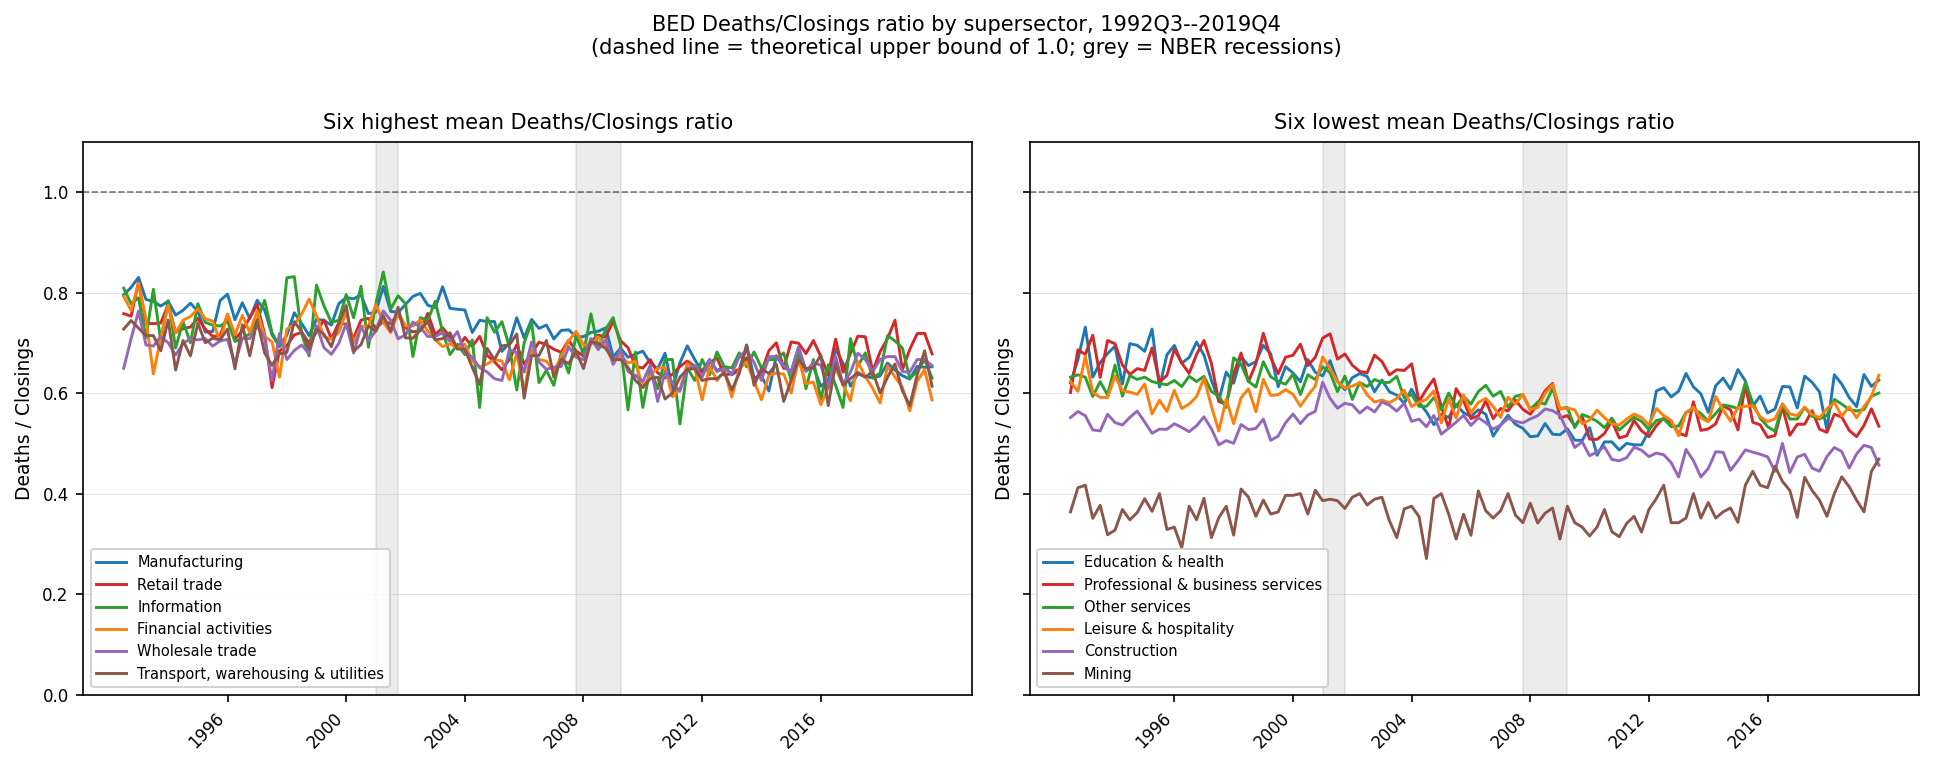
\includegraphics[width=\linewidth]{bed_deaths_by_supersector.png}
		\caption{BED Deaths/Closings ratio by supersector, 1992Q3--2019Q4.
			\emph{Left panel:} six supersectors with highest mean ratio.
			\emph{Right panel:} six supersectors with lowest mean ratio.
			Dashed horizontal line at 1.0 is the theoretical upper bound
			(Deaths $\subseteq$ Closings by construction).
			Grey shading denotes NBER recessions.}
		\label{fig:deaths_by_supersector}
	\end{figure}
	\subsection{Residual \texorpdfstring{$\delta$}{delta}--LD correlation}\label{app:delta_ld_corr}

	After v2 residualization the cross-state correlation between the $\delta$
	and layoffs-and-discharges instruments is
	$r(\tilde{B}^\delta, \tilde{B}^{\text{LD}}) = 0.334$, down from $0.54$
	on raw rates.  The residualization controls for aggregate productivity
	growth, lagged industry value-added, and lagged labor-market tightness,
	ruling out the most obvious industry-demand and aggregate-cycle
	explanations for the shared variation.  The leading interpretation is
	industry-specific financial conditions: when credit tightens in a sector,
	both product-line exit ($\uparrow \delta$) and layoffs at surviving
	establishments ($\uparrow \text{LD}$) rise simultaneously, generating
	positive covariance without a structural link between the two shocks.
	Consistent with this, the Granger-causality evidence shows that $\delta$
	predicts future LD at horizons $h = 4$--$12$ while LD predicts future
	$\delta$ only at $h = 0$--$4$; the long-horizon dependence runs from
	destruction to layoffs and not the reverse.  A natural further step
	would be to residualize on a measure of sector-level credit supply,
	such as SLOOS net C\&I tightening interacted with industry leverage
	exposure; we leave this for future work.

	\subsection{LD local projections}\label{app:ld_lp}

	The separate LD local projections are subsumed by the joint LP figure
	(Figure~\ref{fig:joint_lp_vacancy} below), which overlays the LD
	separate-specification IRF alongside the joint-LP coefficient for the
	same instrument.  In the separate specification the LD unemployment
	response rises monotonically to a peak of $+1.68$ pp at $h=20$,
	significant throughout, while the vacancy response is persistently
	negative (trough $-0.45$ pp at $h=20$).  Both patterns survive the
	severity placebo.  The monotonically rising unemployment IRF is
	anomalous given the estimated LD persistence
	$\hat\rho_{\text{LD}} \approx 0.3$: a transitory shock should produce
	a hump-shaped response, not a path that continues to rise five years
	out.  The most likely explanation is GFC contamination --- the 2008--09
	recession produced a severe and prolonged layoff episode whose
	industry-composition variation is not fully absorbed by the v2
	residualization --- rather than a structural property of the $s$ shock.
	We regard the LD IRFs as indicative rather than structural, and do not
	use them as estimation targets.

	\subsection{Joint local projection}\label{app:joint_lp}

	Figure~\ref{fig:joint_lp_vacancy} reports the joint versus separate
	local projections for the vacancy outcome.  Each panel overlays the
	joint-LP coefficient (red, solid) against the corresponding
	separate-LP coefficient (blue, solid), with 90\% confidence bands.

	\begin{figure}[H]
		\centering
		
\includegraphics[width=\textwidth]{lp_joint_delta_ld_vacancy.png}
		\caption{Joint versus separate local projections: vacancy rate
			outcome.  \emph{Left panel:} $\delta$ instrument --- joint LP
			(red) vs.\ separate LP (blue).  \emph{Right panel:} LD
			instrument --- joint LP (red) vs.\ separate LP (blue).
			Shading denotes 90\% confidence intervals; standard errors
			clustered at the state level ($n=50$).  Instruments are
			v2-residualized; sample 2001Q1--2019Q4.}
		\label{fig:joint_lp_vacancy}
	\end{figure}

	Three findings emerge from the figure.  First, the $\delta$ vacancy IRF
	is qualitatively stable across specifications: the joint and separate
	coefficients share the same sign, timing, and shape throughout, and the
	confidence bands overlap at most horizons.  The trough in the joint
	specification ($-0.535$ pp at $h=5$) is somewhat shallower and earlier
	than in the separate specification ($-0.582$ pp at $h=18$), reflecting
	partial absorption of the shared variation with LD, but the persistent
	negative response to product-line destruction is not an artifact of LD
	exposure.

	Second, the $\delta$ unemployment IRF shrinks by roughly $0.6$--$0.8$
	pp in the joint specification relative to the separate LP, reflecting
	absorption of the variation that $\tilde{B}^\delta$ and
	$\tilde{B}^{\text{LD}}$ share.  The joint peak of $+1.15$ pp remains
	positive and significant, so the unemployment result is robust, if
	attenuated.

	Third, the LD vacancy coefficient collapses from its separate-LP value
	to approximately zero and is insignificant at all horizons once
	$\delta$ is controlled for (right panel).  This collapse should
	\emph{not} be read as evidence that $\delta$ subsumes a genuine LD
	effect on vacancies.  Rather, it reflects that
	$r(\tilde{B}^\delta,\tilde{B}^{\text{LD}})=0.334$ is large enough that
	the two instruments do not span orthogonal directions in the shock
	space: the variation in $\tilde{B}^{\text{LD}}$ orthogonal to
	$\tilde{B}^{\delta}$ is insufficient to separately identify the LD
	vacancy response.  The appropriate conclusion is that LD is not
	separately identified as a structural shock in this setting, not that
	separation shocks have zero causal effect on vacancies.

	We therefore treat the separate $\delta$ LP as the primary
	specification.  The joint LP establishes that the headline result ---
	a persistent vacancy decline in response to product-line destruction
	--- is robust to controlling for LD, and that the failure to separately
	identify LD is an instrument-space problem rather than a finding about
	vacancy dynamics.

	\subsection{QU placebo instrument}\label{app:qu_placebo}

	$\tilde{B}^{\text{QU}}$ is constructed from JOLTS quit rates using the
	same shares and residualization as the primary instruments.  Quits
	represent voluntary job-to-job transitions: the quitting worker moves
	directly to another employer, leaving the origin firm with an unfilled
	position but supplying the destination firm with a worker.  The net
	effect on aggregate unemployment and vacancies is therefore ambiguous
	and governed by matching frictions at the destination, not by the
	separation event at the origin.  This is conceptually distinct from the
	model's $s$ shock, which dissolves a match and triggers an unambiguous
	vacancy repost.  Furthermore, the quit rate is procyclical --- it rises
	when labor markets tighten --- so $\tilde{B}^{\text{QU}}$ partly
	reflects the same industry-level demand cycle that v2 residualization
	attempts to remove.

	Empirically, the QU instrument does not behave as a flat-zero placebo.
	Its unemployment and vacancy IRFs are nearly identical in magnitude to
	those of $\tilde{B}^\delta$, and the within-instrument correlation
	$\text{corr}(\hat\beta^u_h, \hat\beta^v_h) = -0.971$ across $h =
	0,\ldots,20$ --- the same mechanical proportionality observed for
	$\tilde{B}^\delta$ ($-0.948$).  This signature indicates that QU
	identifies industry-level demand contractions (which move $u$ and $v$
	symmetrically along the Beveridge curve) rather than a structurally
	distinct separation shock.  The contamination is likely structural:
	high-quit industries tend to be procyclical, so the industry component
	of the quit rate is correlated with demand conditions even after
	residualization on aggregate productivity and lagged VA.  The QU
	failure confirms that a well-identified $s$-type instrument remains an
	open challenge and motivates treating the LD results as indicative
	rather than structural.

	%%%%%%%%%%%%%%%%%%%%%%%%%%%%%%%%%%%%%%%%%%


	\section{Steady state}\label{app:steady_state}
	We summarize the steady state of the system below:
	\begin{align}
		%	p&=N^{1/(\varepsilon-1)}\\
		\nu^f&=\rho(N)f_e/\mu(N)\\
		w^{int}&=\rho(N)z/\mu(N)\\
		\frac{d^f}{\nu^f}&=\frac{r+\delta_e}{1-\delta_e}\\
		\kappa+\frac{K}{q(\theta)}&=\frac{1-\delta_e}{r+\tau}(w^{int}-w-K)\\
		%\frac{\gamma P}{q(\theta)}&=\frac{z/\mu-w}{\rho+s}\\
		%\gamma N^{1/(1-\varepsilon)}\left[\frac{\rho+s}{q(\theta)}+\phi \theta\right]&=(1-\phi)\left(pz/\mu-b-K\right)\\
		w &= \phi \left[ w^{int}-K+\theta(K+q(\theta)\kappa)\right]+(1-\phi)b\\
		Q&=e^{1/\xi}x_m \\
		1-\delta_e&=(1-\delta)F(x^c),\quad \tau=1-(1-\delta_e)(1-s)\\
		K&=\frac{r+\delta_e}{1+r}Q\\
		u&=\frac{\tau}{\tau+(1-\delta_e)f(\theta)}\label{eq:u_ss}\\
		e&=\delta_e(v+1-u)\label{eq:e_ss}\\
		N^e&=\delta_e N/(1-\delta_e)\\
		L^c&=\frac{r+\delta_e}{r+\delta_e+\delta_e \pi_s \mu}L,\quad L^e=\frac{\delta_e \pi_s \mu}{r+\delta_e+\delta_e\pi_s L \mu}\label{eq:labor_ss}\\
		x^c&=\frac{\rho f_e}{\mu}\left(\frac{r+\delta_e}{1-\delta_e}\frac{\mu-1}{\mu \pi_s}+1\right)\\
		\pi_s&=\frac{\mu-1}{\mu}\frac{(1-\psi_c)(r+\delta_e)}{r+\delta_e+\psi_c(1-\delta_e)}\\
		Y^{Gross}&=Y^C+\nu^f N^e=w^{int}L+Nd^f\\
		Y&=C+\nu^fN^e\\
		X&=e\frac{\xi}{\xi+1}Q+\kappa qv\\
		X^c&=N\psi_c x^c\\
		Y^c&=\rho zL^c=C+X+X^c\\
	\end{align}
	Most of these equations are self-evident from the equilibrium system. For instance, evaluating \eqref{eq:u_lom} yields \eqref{eq:u_ss}. To find $e$, start with the steady-state vacancy law of motion:
	\begin{align}
		[1-(1-\delta_e)(1-q)]v=(1-\delta_e)s(1-u)+e
	\end{align}
	Expanding the left-hand side as $\delta_e v+(1-\delta_e)qv$ and rewriting $(1-\delta_e)qv=\tau(1-u)$, we have
	\begin{align}
		\delta_e v+\tau(1-u)=(1-\delta_e)s(1-u)+e\\
		\delta_e v + [\tau-(1-\delta_e)s](1-u)=e
	\end{align}
	so $e=\delta_e(v+1-u)$. Equation~\eqref{eq:e_ss} makes clear how the contribution of new entrants to the vacancy pool is governed by the total exit rate $\delta_e$.
	
	To find labor in entry $L^e$ in terms of aggregate labor, \eqref{eq:labor_ss}, we plug the resource constraint curve into the expression for $L$:
	\begin{align}
		L^e&=\frac{\delta_e}{1-\delta_e}Nf_e/z\\
		&=\frac{\delta_e}{1-\delta_e}\left[\frac{(\mu-1)zL(1-\delta_e)}{f_e(\delta_e \mu+r)}\right]f_e/z\\
		&=\frac{\delta_e(\mu-1)}{\delta_e \mu+r}L
	\end{align}
	The steady-state job creation and wage equations can be arranged as
	\begin{align}\label{eq:jcc_wage_ss}
		\kappa+\frac{K}{q}=\frac{1-\delta_e}{r+\tau}\left[(1-\phi)(w^{int}-K-b)-\phi \theta q\!\left(\kappa+\frac{K}{q}\right)\right]
	\end{align}
	Equation \eqref{eq:jcc_wage_ss} equates the average recruiting cost to the present-discounted value of the match, adjusted for the wage bargain. The right-hand side incorporates a fraction $1-\phi$ of the flow surplus $(w^{int}-K-b)$ and an adjustment for the outside option of the worker. Whereas in the standard DMP model, the analogous expression would characterize tightness, here $K$ and $w^{int}$ are additional endogenous variables. Moreover, the average recruiting cost has the compound form $\kappa+K/q$, and discounting is adjusted by the overall firm survival rate $1-\delta_e$.
	
	\section{Derivations}
	\subsection{Relationship between profit share and Power law shape parameter $\psi$} 
	Here, we can establish the relationship between $\pi_s$ and $\psi_c=\psi/(1+\psi)$. and the probability of a positive fixed cost $p_0$. Recall that the cutoff satisfies $x^c=Y^c[(\mu-1)/(\mu N)]+\rho f_e/\mu$. So, aggregate fixed costs are $X^c=\psi_c p_0(Y^c(\mu-1)/\mu+N\rho f_e/\mu)$.
	Divide by $Y^c$ and use $Y^c=\rho z L^c$ to show that
	\begin{align}
		\frac{X^c}{Y^c}=\frac{\psi_c p_0}{\mu}\left(\mu-1+\frac{f_eN}{zL^c}\right)
	\end{align}
	Now, plug in \eqref{eq:labor_C_N} to show
	\begin{align}
		\frac{X^c}{Y^c}=\frac{\psi_c p_0}{\mu}\left(\mu-1+\frac{1-\delta_e}{r+\delta_e}\mu \pi_s\right)
	\end{align}
	Hence, 
	\begin{align}
		\pi_s=\frac{\mu-1}{\mu}(1-\psi_c p_0)-\frac{\psi_c p_0(1-\delta_e)\pi_s}{r+\delta_e}
	\end{align}
	We solve for $\pi_s$ as
	\begin{align}\label{eq:profit_share}
		\pi_s=\frac{\mu-1}{\mu}\frac{(1-\psi_cp_0)(r+\delta_e)}{r+\delta_e+\psi_cp_0(1-\delta_e)}
	\end{align}
	It is easy to verify that, holding $\delta_e$ fixed, $\pi_s$ is increasing with $\psi_c$. In particular, for $\psi_c=0, \pi_s=(\mu-1)/\mu=1/\varepsilon$, as \citet{bilbiie_2012}. 
	We can rewrite the cutoff $x^c$ in terms of both the profit share and $\psi_c p_0$:
	\begin{align}
		x^c&=\frac{\rho}{\mu}\left(\frac{zL^c(\mu-1)}{N}+f_e\right)\\
		&=\frac{\rho f_e}{\mu}\left(\frac{r+\delta_e}{1-\delta_e}\frac{\mu-1}{\mu \pi_s}+1\right)\\
		&=\frac{\rho f_e}{\mu}\left(\frac{r+\delta_e}{1-\delta_e}\frac{r+\delta_e+\psi_cp_0(1-\delta_e)}{(1-\psi_cp_0)(r+\delta_e)}+1\right)
	\end{align}
	
	\subsection{Resource constraint curve}
	Expressing the $N$--$L$ relationship in terms of the distributional parameter $\psi_c$, rearrange~\eqref{eq:labor_N} as 
	\begin{align}
		N=\frac{ zL(1-\delta_e)}{f_e\left(\frac{r+\delta_e}{\mu \pi_s}+\delta_e\right)}
	\end{align}
	Substitute the value $\pi_s$ from \eqref{eq:profit_share} to obtain
	\begin{align}
		N=\frac{zL(\mu-1)(1-\psi_c p_0)}{f_e[r+\delta_e+\psi_c(1-\delta_e)+\delta_e (\mu-1)(1-\psi_c)]}
	\end{align}
	
	Hence, labor in entry is
	\begin{align}
		L^e&=\frac{\delta_e}{1-\delta_e}\frac{Nf_e}{z}\\
		&=\frac{\delta_e(\mu-1-\psi_c p_0)L}{\delta_e \mu+r+\psi_c p_0(1-\mu \delta_e)}
	\end{align}
	Thus, labor in the consumption sector is
	\begin{align}
		L^c=\frac{r+\delta_e+\psi_c p_0(1-(\mu-1)\delta_e)}{\delta_e\mu+r+\psi_c p_0(1-\mu \delta_e)}L
	\end{align}
	We can substitute to solve for $X^c$ as
	\begin{align}
		X^c&=\frac{\rho z L}{\mu}\psi_c p_0\left(\mu-1+\frac{(\mu-1-\psi_c p_0)(1-\delta_e \mu)}{\delta_e \mu+r+\psi_c p_0(1-\mu \delta_e)}\right)\\
	\end{align}
	Hence, the ratio $X^c/Y^c$ satisfies
	\begin{align}
		\frac{X^c}{Y^c}=\frac{L}{L^c}\frac{\psi_c p_0}{\mu}\left(\mu-1+\frac{(\mu-1-\psi_cp_0)(1-\delta_e \mu)}{\delta_e \mu+r+\psi_c p_0(1-\mu \delta_e)}\right)
	\end{align}
	%\eqref{eq:curve_res_cons}.
	\subsection{Labor share of GDP}
	The aggregate resource constraint can be rearranged to pin down the income of recruiters:
	\begin{align}
		w^{int}L=\frac{Y^c}{\mu}+\nu^f N^e
	\end{align}
	Thus, the income share of recruiters relative to gross output is
	\begin{align}
		\frac{w^{int}L}{Y^{Gross}}&=\pfrac{r+\delta_e}{r+\delta_e+\delta_e \pi_s}\frac{1}{\mu}+\frac{\delta_e\pi_s}{r+\delta_e+\pi_s}\\
		&=\frac{r+\delta_e+\delta_e \mu \pi_s}{\mu(r+\delta_e+\delta_e\pi_s)}
	\end{align}
	The labor share of GDP is
	\begin{align}
		\frac{wL}{Y} = (1+\frac{X+X^c}{Y})\frac{w}{w^{int}}\frac{r+\delta_e+\delta_e \mu \pi_s}{\mu(r+\delta_e+\delta_e\pi_s)}
	\end{align}
	The steady-state labor share is composed of three factors. The first factor just reflects the wedge between gross output and GDP, which depends on the recruiting cost and fixed cost shares. The second and third comprise a search wedge $w/w^{int}$ and a market power wedge $w^{int}L/Y^{Gross}$. Through the latter, the labor share depends positively on $\delta_e$ and $\rho$, and negatively on $\pi_s$. Intuitively, a higher product destruction rate requires more labor resources, and thus income accruing to labor. A higher price markup raises profits and thus lowers the labor share. Indeed, in standard DSGE models with monopolistic competition, the labor share just the inverse of the price markup. Here that arises as a limiting case in which search frictions vanish ($w\to w^{int}$) and $\delta \to 0$. The latter entails eliminating the entry sector, which affects the labor share since only retailers charge markups. Note that the search wedge, in turn, depends on $\phi$ and $b$. Moreover, variety effects affect the search wedge through $w^{int}$ but otherwise do not affect the steady-state shares.
	
	The special case studied by \citet{bilbiie_2012} arises if we shut down labor market frictions and fixed costs in production. In this limit $\delta_e=\delta$ (no endogenous exit), $w^{int}=w$, $X=X^c=0$, and $\pi_s=1/\varepsilon$, giving
	\begin{align}
		\frac{wL}{Y}=\frac{(r+\delta)(\varepsilon-1)+\delta}{\varepsilon(r+\delta)+\delta}=\frac{C}{Y}\frac{1}{\mu}+\frac{\nu^f N^e}{C}
	\end{align}
	which equals the consumption share divided by the markup plus the entry share.
	
	\subsection{Wage determination}
	We characterize the wage $w_t$. To characterize these value functions, we revisit the value of the large household:
	\begin{align}
		W_t&=\max_{c_t,a_t} \frac{c_t^{1-\sigma}}{1-\sigma}+\beta \mathbb{E}_t W_{t+1} \quad \text{s.t.}\\
		&c_t+\nu_ta_{t+1}=w_tL_t+b(1-L_t)+(\nu_t+d_t)a_t+D_t^{int} -T_t
	\end{align}
	Note that, given the continuum of members in a household, the surplus of moving an unemployed household into employment is $\der{W_t}{L_t}$. Nash bargaining solves
	\begin{align}\label{eq:Nash_product}
		w_t=\arg \max [\der{W_t(w_t)}{L_t}]^{\phi}[J_t(w_t)-Q_t]^{1-\phi}
	\end{align}
	For convenience, we define the match surpluses $S_T^H = \der{W_t}{L_t}$. and $S_t^J=J_t-Q_t$.
	
	From the Bellman equation,
	\begin{align} \label{eq:Nash_rule}
		\der{W_t}{L_t}=c_t^{-\sigma}\der{c_t}{L_t}+\beta \mathbb{E}_t[\der{W_{t+1}}{L_{t+1}}\der{L_{t+1}}{L_t}]
	\end{align}
	From the budget constraint, $\der{c_t}{L_t}=w_t-b$. Moreover, given the law of motion of employment $L_{t+1}=(1-\delta_t)[f(\theta_t)(1-L_t)+(1-s_t)]L_t$, we have
	\begin{align}
		\der{L_{t+1}}{L_t}=(1-\delta_t)(1-s_t-f(\theta_t))
	\end{align}
	Putting it together, we have
	\begin{align}
		S_t^H=c_t^{-\sigma}(w_t-b)+\beta(1-\delta_t)(1-s_t-f(\theta_t))\mathbb{E}_tS_{t+1}^H
	\end{align}
	The first-order condition of the Nash product \eqref{eq:Nash_product} is
	\begin{align}
		\phi \frac{\der{S_t^H}{w_t}}{S_t^H}+(1-\phi)\frac{\der{J_t}{w_t}}{J_t}=0
	\end{align}
	We evaluate
	\begin{align}
		\der{S_t^H}{w_t}=\der{[u'(c_t)(w_t-b)]}{w_t}+\beta(1-\delta_t)(1-s_t-f(\theta_t))\der{}{w_t}\mathbb{E}_tS_{t+1}^H
	\end{align}
	The term $\der{}{w_t}\mathbb{E}_tS_{t+1}^H=0$ because the next-period wage is re-bargained based on next period conditions. Thus, $\der{S_t^H}{w_t}=c_t^{-\sigma}$.
	Recall that the firm surplus is
	\begin{align}
		S_t^J=w_t^{int,j}-w_t-K_t +(1-s_t)\left(\kappa+\frac{K_t}{q(\theta_t)}\right)
	\end{align}
	Note that $\der{S_t^J}{w_t}=-1$, so we obtain the sharing rule
	\begin{align}
		S_t^H=\frac{\phi}{1-\phi}c_t^{-\sigma}S_t^J
	\end{align}
	%The solution has the form $\der{W_t}{w_t}=(\phi/(1-\phi))J_t$.
	%Recognizing that $\der{W_t}{w_t}c_t^{-\sigma}=\der{W_t}{L_t}$, we have
	
	From \eqref{eq:average_hiring_cost},
	\begin{align}
		\mathbb{E}_t\beta(1-\delta_t)\pfrac{c_{t+1}}{c_t}^{-\sigma}S_{t+1}^J=\kappa+\frac{K_t}{q(\theta_t)}
	\end{align}
	Nash bargaining at period $t+1$ corresponds to \eqref{eq:Nash_rule} forwarded one period.
	Hence,
	\begin{align}
		\beta (1-\delta_t) \mathbb{E}_tS_{t+1}^H=\frac{\phi}{1-\phi}c_t^{-\sigma}\left(\kappa+\frac{K_{t}}{q(\theta_{t})}\right)
	\end{align}
	We can rewrite the household surplus as
	\begin{align}
		S_t^H=c_t^{-\sigma}(w_t-b)+(1-s-f(\theta_t))\frac{\phi}{1-\phi}c_t^{-\sigma}\left(\kappa+\frac{K_{t}}{q(\theta_{t})}\right)
	\end{align}
	Now, we wish to substitute out $S_t^H$. To do so, we combine the expressions for recruiter surplus and bargaining:
	\begin{align}
		S_t^J&=w_t^{int}-w_t-K_t+(1-s_t)\left(\kappa+\frac{K_t}{q(\theta_t)}\right)\\
		S_t^J&=\frac{1-\phi}{\phi}c_t^{\sigma}S_t^H
	\end{align}
	so that
	\begin{align}
		w_t^{int}-w_t-K_t+(1-s_t)\left(\kappa+\frac{K_t}{q(\theta_t)}\right)=\frac{1-\phi}{\phi}\left(w_t-b+(1-s-f(\theta_t))\frac{\phi}{1-\phi}\left(\kappa+\frac{K_t}{q(\theta_t)}\right)\right)
	\end{align}
	This expression can be rearranged explicitly for the wage:
	\begin{align}
		w_t=\phi\left(w_t^{int}-K_t+f(\theta_t)\left(\kappa+\frac{K_t}{q(\theta_t)}\right)\right)+(1-\phi)b
	\end{align}
\section{Limiting cases}
\label{app:limiting_cases}

\subsection*{Proof of Proposition~\ref{prop:independence}}

We establish the if-and-only-if by showing necessity 
and sufficiency of each condition separately.

\paragraph{Sufficiency}
Set $\sigma=0$, $\zeta=0$, $p_0=0$. Under $\sigma=0$, 
the stochastic discount factor reduces to 
$m_{t+1}=\beta$, eliminating dependence on 
consumption $C_t$ from all intertemporal conditions. 
Under $\zeta=0$, general CES preferences give 
$\rho(N_t)=1$ for all $N_t$, so recruiter 
compensation $w_t^{int}=\rho(N_t)z_t/\mu(N_t) = 
z_t/\mu$ depends on $N_t$ only through $\mu(N_t)$; 
but under general CES with $\zeta=0$, $\mu$ is a 
constant independent of $N_t$, so $w_t^{int}=z_t/\mu$ 
is exogenous to the labor market block. Under $p_0=0$, 
$\Lambda_t = F_\chi(\chi_t^c) = 1-p_0 = 1$ for all 
$\chi_t^c$, so $\delta_{e,t}=1-(1-\delta_{t-1})\Lambda_t 
= \delta_{t-1}$ depends only on the exogenous shock.

Under all three conditions, inspect the labor market 
block \eqref{eq:jcc_eq}--\eqref{eq:entry_eq} and 
laws of motion \eqref{eq:v_lom}--\eqref{eq:u_lom}. 
With $m_{t+1}=\beta$, $w_t^{int}=z_t/\mu$, and 
$\delta_{e,t}=\delta_{t-1}$, these equations form 
a closed system in 
$\{u_{t+1},v_t,e_t,Q_t,K_t,w_t\}_{t=0}^\infty$ 
given exogenous states $\{z_t,\delta_t,s_t\}$ and 
initial conditions $\{v_{-1},u_0\}$. No variable 
from the business formation block 
$\{N_t,C_t,Y_t^c,\chi_t^c\}$ appears. The labor 
market block is therefore self-contained.

Given the solution to the labor market block, 
the business formation block 
\eqref{eq:N_lom_eq}--\eqref{eq:cutoff_eq} 
determines $\{N_t,C_t,Y_t^c,\chi_t^c\}$ taking 
$\{u_t,X_t\}$ as given. This confirms the 
recursive structure.

\paragraph{Necessity}
We show that relaxing any single condition 
breaks separability.

\emph{$\sigma>0$}: With $\sigma>0$, 
$m_{t+1}=\beta(C_{t+1}/C_t)^{-\sigma}$ depends on 
$C_t$, which is determined by the resource 
constraint \eqref{eq:rc} jointly with $N_t$, 
$X_t^c$, and $Y_t^c$. The job creation condition 
\eqref{eq:jcc_eq} and flow vacancy value 
\eqref{eq:Kdef} both contain $m_{t+1}$, so the 
labor market block depends on $C_t$ and hence on 
the business formation block.

\emph{$\zeta>0$}: With $\zeta>0$, $\rho(N_t)>1$ 
for $N_t>1$ and $\rho'(N_t)>0$, so 
$w_t^{int}=\rho(N_t)z_t/\mu(N_t)$ depends on $N_t$. 
Since $N_t$ is determined in the business formation 
block, the job creation condition \eqref{eq:jcc_eq} 
depends on $N_{t+1}$ through $w_{t+1}^{int}$, 
breaking separability.

\emph{$p_0>0$}: With $p_0>0$, 
$\Lambda_t=F_\chi(\chi_t^c)<1$ for $\chi_t^c<\chi_m$, 
and $\chi_t^c$ satisfies the cutoff condition 
\eqref{eq:cutoff_eq} which depends on $Y_t^c$, 
$N_t$, and $\mu(N_t)$ --- all determined in the 
business formation block. Hence 
$\delta_{e,t}=1-(1-\delta_{t-1})\Lambda_t$ depends 
on business formation variables. Since $\delta_{e,t}$ 
enters both laws of motion 
\eqref{eq:v_lom}--\eqref{eq:u_lom}, the labor 
market block depends on the business formation 
block. \hfill$\square$

\subsection*{Proof of Proposition~\ref{prop:double_limit}}

Consider the DS-CES equilibrium with $p_0=0$ and 
parameters $(\varepsilon, f_e)$ satisfying 
$f_e=\bar{f}_e/\varepsilon$ for fixed $\bar{f}_e>0$. 
Since $p_0=0$, $\Lambda_t=1$ and 
$\delta_{e,t}=\delta_{t-1}$ throughout. We establish 
claims (iii), (iv), (i), and (ii) in that order, 
since (iii) is used in (iv) and (i) validates an 
assumption used in (iii).

\paragraph{Claim (iii): $w_t^{int}\to z_t$.}
Under DS-CES, $\mu=\varepsilon/(\varepsilon-1)\to 1$ 
and $\rho(N_t)=N_t^{1/(\varepsilon-1)}$. For any 
$N_t$ satisfying $N_t = O(e^{o(\varepsilon)})$ as 
$\varepsilon\to\infty$ --- a condition weaker than 
boundedness, verified below --- 
$\ln\rho(N_t) = \ln N_t/(\varepsilon-1)\to 0$, so 
$\rho(N_t)\to 1$. Hence 
$w_t^{int}=\rho(N_t)z_t/\mu(N_t)\to z_t$ along 
any such equilibrium path. $\square$

\paragraph{Claim (iv): $N_t$ drops out of aggregate 
	allocations.}

We show that $\{\theta_t, u_t, v_t, C_t, Y_t^c\}$ 
are determined independently of $N_t$ in the limit.

\emph{Labor market block.} From claim (iii), 
$w_t^{int}\to z_t$. Since $p_0=0$ gives $\Lambda_t=1$, 
the job creation condition \eqref{eq:jcc_eq}, flow 
vacancy value \eqref{eq:Kdef}, free entry 
\eqref{eq:entry_eq}, and laws of motion 
\eqref{eq:v_lom}--\eqref{eq:u_lom} converge to 
\eqref{eq:jcc_ags}--\eqref{eq:u_ags}, which contain 
no reference to $N_t$.

\emph{Resource constraint.} Since $p_0=0$, 
$X_t^c=0$. Labor devoted to entry satisfies 
$l_t^e = f_e N_t^e/z_t = O(1/\varepsilon)\to 0$, 
established in claim (ii). Hence 
$L_t^c = L_t - l_t^e \to L_t = 1-u_t$. 
Output per firm $y_t = z_t L_t^c/N_t \to 
z_t(1-u_t)/N_t$, and $Y_t^c = \rho(N_t)N_t y_t 
\to 1\cdot N_t\cdot z_t(1-u_t)/N_t = z_t(1-u_t)$. 
The resource constraint becomes 
$C_t = z_t(1-u_t)-X_t$, independent of $N_t$.

Since all equations determining 
$\{\theta_t,u_t,v_t,C_t,Y_t^c\}$ are independent 
of $N_t$ in the limit, the normalization $\bar{N}=1$ 
is a units convention for the measure of product 
lines --- analogous to normalizing household measure 
to unity --- and involves no loss of generality for 
aggregate allocations. No restriction on $\bar{f}_e$ 
is required to implement it. $\square$

\paragraph{Claim (i): steady-state value of $N_t$.}

Since aggregate allocations are independent of 
$N_t$ by claim (iv), the dynamic path of $N_t$ 
does not affect the proposition's main result. We 
nonetheless characterize the steady state and 
local dynamics of $N_t$ to confirm it remains 
well-defined in the limiting economy.

Substituting $f_e=\bar{f}_e/\varepsilon$ and 
$\rho(N_t)=N_t^{1/(\varepsilon-1)}$ into the firm 
LOM \eqref{eq:N_lom_eq} with $p_0=0$ and taking 
$\varepsilon\to\infty$, using the approximation 
$N^{-1/(\varepsilon-1)} = e^{-\ln N/(\varepsilon-1)} 
\approx 1-\ln N/(\varepsilon-1)$:
\begin{align}\label{eq:N_lom_limit}
	N_t \to (1-\delta_{t-1})
	\left(N_{t-1} + \frac{z_{t-1}(1-u_{t-1})
		\ln N_{t-1}}{\bar{f}_e}\right)
\end{align}
This is a nonlinear predetermined variable equation 
driven by the exogenous processes 
$\{z_t,\delta_t,u_t\}$, with no forward-looking 
terms. Its unique positive steady state 
$\bar{N}$ satisfies:
\begin{align}\label{eq:N_ss_limit}
	\bar{\delta}\bar{N} = 
	\frac{\bar{z}\bar{L}\ln\bar{N}}{\bar{f}_e}
\end{align}
where $\bar{L}=1-\bar{u}$. The right-hand side 
is zero at $\bar{N}=1$, strictly positive and 
increasing for $\bar{N}>1$, while the left-hand 
side is linear with positive slope $\bar{\delta}$. 
A unique solution $\bar{N}>1$ exists for any 
$\bar{\delta},\bar{f}_e,\bar{z},\bar{L}>0$ by 
the intermediate value theorem and strict 
monotonicity.

Linearizing \eqref{eq:N_lom_limit} around 
$\bar{N}$ gives autoregressive coefficient:
\begin{align}
	\rho_N \equiv (1-\bar{\delta})
	\left(1+\frac{\bar{z}\bar{L}}
	{\bar{f}_e\bar{N}}\right)
	= (1-\bar{\delta})
	\left(1+\frac{\bar{\delta}}{\ln\bar{N}}\right)
\end{align}
where the second equality uses 
\eqref{eq:N_ss_limit}. Local stability requires 
$\rho_N < 1$, which holds if and only if 
$\bar{N} > e^{1-\bar{\delta}}$. For 
$\bar{\delta}\approx 0.05$, this requires 
$\bar{N}>e^{0.95}\approx 2.59$ --- satisfied for 
sufficiently small $\bar{f}_e$ given other 
parameters. When the stability condition holds, 
$N_t$ follows a well-defined stationary process 
driven by $\{z_t,\delta_t,u_t\}$, confirming the 
path satisfies $N_t=O(e^{o(\varepsilon)})$ as 
required by claim (iii). $\square$

\paragraph{Claim (ii): rates of convergence.}

\emph{Firm value}: $\nu_t^f=\rho(N_t)f_e/\mu(N_t) 
\approx 1\cdot(\bar{f}_e/\varepsilon)\cdot 1 = 
O(1/\varepsilon)$.

\emph{Investment}: At steady state, 
$N_t^e=\bar{\delta}\bar{N}/(1-\bar{\delta})=O(1)$, 
so $\nu_t^f N_t^e = O(1/\varepsilon)\cdot O(1) 
= O(1/\varepsilon)$.

\emph{Labor to entry}: $l_t^e=f_eN_t^e/z_t = 
(\bar{f}_e/\varepsilon)\cdot O(1)/z_t = 
O(1/\varepsilon)$. $\square$

\subsection*{Proof of Proposition~\ref{prop:ags}}

Under clone replacement, $N_t=1$ and $\mu=1$ are 
maintained by construction at all times. We verify 
that the business formation block drops out and 
the remaining system reduces to 
\eqref{eq:jcc_ags}--\eqref{eq:u_ags}.

\emph{Business formation block.} Substituting 
$N_t=1$ and $\mu=1$ into the baseline equilibrium 
definition:

The firm LOM \eqref{eq:N_lom_eq}: with $N_t=1$ 
maintained by construction, this equation is 
satisfied trivially by the clone replacement 
assumption and imposes no restriction on other 
variables.

The business formation Euler \eqref{eq:N_euler_eq}: 
with $\rho(1)=1$, $\mu(1)=1$, $f_e\rho(N_t)=f_e$, 
and $(\mu(N_{t+1})-1)=0$, the right-hand side 
reduces to $(1-\delta_t)\mathbb{E}_t m_{t+1}\Lambda_{t+1}
\{f_e\}=f_e\cdot(1-\delta_t)\mathbb{E}_t m_{t+1}$. 
This is a condition on $f_e$ alone and is satisfied 
by appropriate choice of $f_e$ given $\beta$ and 
$\bar{\delta}$; it imposes no restriction on labor 
market variables.

The cutoff condition \eqref{eq:cutoff_eq}: with 
$\mu=1$, $(\mu-1)/\mu=0$, so 
$\chi_t^c = f_e\rho(N_t)/\mu(N_t) = f_e$. Since 
clone replacement maintains $N_t=1$ regardless of 
profitability, the exit decision is moot; 
$\chi_t^c=f_e$ is a constant that imposes no 
restriction on aggregate allocations.

The resource constraint \eqref{eq:rc}: since 
$p_0=0$ under clone replacement (endogenous exit 
is absent by construction), $X_t^c=0$. With 
$\rho(1)=1$ and $\mu(1)=1$, $Y_t^c=z_t(1-u_t)$ 
and $l_t^e=0$, giving $C_t=z_t(1-u_t)-X_t$, 
which is \eqref{eq:rc_limit}.

\emph{Labor market block.} Substituting $\rho(N_t)=1$, 
$\mu(N_t)=1$, $\Lambda_t=1$, and 
$\delta_{e,t}=\delta_{t-1}$ into 
\eqref{eq:jcc_eq}--\eqref{eq:u_lom} yields 
\eqref{eq:jcc_ags}--\eqref{eq:u_ags} directly. 
The stochastic discount factor 
$m_t=\beta(C_t/C_{t-1})^{-\sigma}$ is unchanged. 
The stochastic processes \eqref{eq:ar1_z}--\eqref{eq:ar1_s} 
are unchanged.

The resulting system
\eqref{eq:jcc_ags}--\eqref{eq:u_ags} together
with $e_t=G(Q_t)$, $m_t=\beta(C_t/C_{t-1})^{-\sigma}$,
$C_t=z_t(1-u_t)-X_t$, and stochastic processes
\eqref{eq:ar1_z}--\eqref{eq:ar1_s} is well-posed:
it inherits a unique bounded equilibrium from
standard DSGE existence conditions, since it is
a special case of the baseline model with
$N_t=1$ fixed, which satisfies the Blanchard-Kahn
conditions on the labor market block established
in the baseline analysis. \hfill$\square$

\subsection*{Proof of Proposition~\ref{prop:bgm_nest}}

Set $p_0=0$. Then $F_\chi(0)=0$, so no firm pays a
continuation cost: $X_t^c=0$, $\Lambda_t=1$, and
$\delta_{e,t}=\delta_{t-1}$ for all $t$.

\emph{Firm LOM~\eqref{eq:N_lom_eq}.} With $\Lambda_t=1$
and $\delta_{e,t}=\delta_{t-1}$, the baseline LOM becomes
\begin{equation*}
  N_t = (1-\delta_{t-1})\!\left(N_{t-1}
  + \frac{z_{t-1}(1-u_{t-1})}{f_e}
  - \frac{Y_{t-1}^c}{f_e\rho(N_{t-1})}\right),
\end{equation*}
where $\{1-u_{t-1}\}$ is treated as an exogenous
sequence by assumption.  Using the gross-output identity
$Y_{t-1}^c = z_{t-1}(1-u_{t-1})\rho(N_{t-1})/\mu(N_{t-1})$
(from retail-firm optimality), the parenthesized term
equals $N_{t-1}^e = z_{t-1}(1-u_{t-1})/f_e \cdot
(1-1/\mu(N_{t-1}))$, which is the BGM entry flow
$N_t^e = G(Q_t)$ evaluated at $Q_t = f_e/\nu_t^f$.
Hence \eqref{eq:N_lom_eq} is the BGM firm LOM.

\emph{Business formation Euler~\eqref{eq:N_euler_eq}.}
With $\Lambda_{t+1}=1$ and $X_{t+1}^c=0$, the baseline
Euler simplifies to
\begin{equation*}
  f_e\rho(N_t) = (1-\delta_t)\,\mathbb{E}_t m_{t+1}
  \frac{\mu(N_t)}{\mu(N_{t+1})}
  \left\{f_e\rho(N_{t+1})
  + \frac{Y_{t+1}^c}{N_{t+1}}(\mu(N_{t+1})-1)\right\}.
\end{equation*}
Dividing by $\rho(N_t)$ and using
$\nu_t^f = f_e\rho(N_t)$ (free entry), this is the BGM
asset-pricing equation for firm equity.

\emph{Resource constraint~\eqref{eq:gdp}.} With
$X_t^c=0$, gross output satisfies $Y_t^c = C_t + X_t$.
Netting out $X_t$ on both sides gives the GDP identity
$Y_t = C_t + \nu_t^f N_t^e$, which is the BGM resource constraint.
The household budget constraint
$c_t = w_t(1-u_t) + \pi_t - X_t$
closes the system identically in both models.

The two systems thus share the same three equations and
the same exogenous sequences $\{z_t,\delta_t,1-u_t,X_t\}$.
Since $1-u_t$ and $X_t$ are endogenous in the baseline but
exogenous in LR-BGM, the proposition asserts isomorphism
for any realization of those sequences, not that the
equilibrium distributions coincide. \hfill$\square$


	\subsection{Details of comparative statics}
	\textcolor{red}{Comment out this section temporarily}
	%In this section, we qualitatively characterize how steady state labor market tightness and firm product lines responds to various shocks under both DS-CES and general-CES preferences.  We analyze the equilibrium in $(\theta,N)$ given by the system \eqref{eq:curve_jcc} and \eqref{eq:curve_res_cons}
	%\begin{align}
	%\left(\kappa+\frac{K(\theta)}{q(\theta)}\right)\left(r+\tau+\phi(1-\delta)\theta q(\theta)\right)&=(1-\delta)(1-\phi)\left(\rho(N)z/\mu-K(\theta)-b\right) \\
	%N&=\frac{(\mu-1)zL(\theta)(1-\delta)}{f_e(\delta \mu+r)}
	%\end{align}
	%%which is graphically represented in \ref{fig:steady_state_curves}.
	%%\begin{figure}[h!]\label{fig:steady_state_curves}
	%%	\centering
	%%	\includegraphics[scale=.3]{steady_state.png}
	%%	\caption{Steady state in $(\theta,N)$.}
	%%\end{figure}
	%
	%where we refer \eqref{eq:curve_jcc} as the job creation (JC) curve and \eqref{eq:curve_res_cons} as the aggregate resource constraint (AC) curve. 
	%
	%Distinct from a standard labor search model, the JC curve includes the flow cost of entry $K(\theta)$ due to finitely elastic vacancy creation.  Futhermore, the number of product lines $N$ is relevant to optimal job creation in that it affects the wage recruiters receive $w^{int}=\rho(N)z/\mu$ through the relative price $\rho(N)$.  In the case of DS-CES preferences $\rho(N)=N^{1/(\epsilon-1)}$ and in the case of general-CES prefences $\rho(N)=N^\zeta$ where $\varepsilon$ is the elasticity of substitution across product lines and $\zeta$ measures agents' desire for variety.  Under both preferences the markup is given by $\mu=\varepsilon/(\varepsilon-1)$.
	%
	%Note that under DS-CES preferences, the limiting case $\epsilon \rightarrow \infty$ in which variety effects are absent, the job creation curve independently determines equilibrium labor market tightness.  That is, the number of product lines is not relevant for vacancy creation.  The resource constraint curve is essentially a market clearing condition which shows the equilibrium level of employment ($L(\theta)$) that a given number of business lines ($N$) can support.  Under general-CES preferences, the limiting case $\zeta \rightarrow 0$ similarly removes variety effects and renders the job creation curve independent of $N$.  With general-CES preferences, however, there can still exist a finite elasticity of substitution since variety effects and the markup are distinct from one another. 
	%
	%When considering steady state comparative statics, the only difference between DS-CES and general-CES preferences is the role of $\rho(N)$ in the job creation curve.  Therefore, with the exception of parameters $\epsilon$ and $\zeta$, all comparative statics are common across the two specifications.  We discuss the common comparative statics first and the role of $\epsilon$ and $\zeta$ last.
	%
	%Consider a positive productivity shock $z$.  Higher productivity increases the real wage recruiters receive $w^{int}=\rho(N)z/\mu$; for a given level of employment $L$ higher aggregate income can support a larger number of businesses.  This is represented by the AC curve shifting upward.  Similarly, higher wages $w^{int}$ increases the surplus received by recruiters; for a given level of business lines $N$ there is more vacancy creation causing a higher level of labor market tightness $\theta$.  This is represented by a rightward shift of the JC curve.  The new equilibrium features both higher tightness and business lines.
	%\begin{figure}[h!]
	%	\centering
	%	\includegraphics[scale=.3]{steady_state_z.png}
	%	\caption{Productivity shock: $z$}
	%\end{figure}
	%
	%Next, consider a positive shock to workers bargaining power $\phi$.  More bargaining power to workers lowers the surplus received by recruiters forcing them to realize higher compensating vacancy filling rates (lower labor market tightness).  This is represented by a leftward shift of the JC curve.  With looser labor markets, movement down along the AC curve shows there is a lower equilibrium level of business lines due to less employment.
	%\begin{figure}[h!]
	%	\centering
	%	\includegraphics[scale=.3]{steady_state_mu.png}
	%	\caption{Bargaining power shock: $\phi$}
	%\end{figure}
	%
	%Notice that an increase in unemployment benefits $b$ will result in the same qualitative effects as an increase in bargaining power.  Rather than shrinking the fraction of the joint surplus recruiters receive, higher unemployment benefits shrinks the joint surplus itself.  Nonethess, it similarly results in lower labor market tightness and fewer product lines.
	%
	%Next, consider a positive shock to fixed entry costs $f_e$.  This shock discourages entry for any given level of tightness and is represented by a downward shift of the AC curve.  Fewer business lines reduce the wage that recruiters receive, through variety effects, causing fewer vacancies to be opened.  This movement down along the JC curve results in lower equilibrium tightness and business lines.
	%\begin{figure}[h!]
	%	\centering
	%	\includegraphics[scale=.3]{steady_state_fe.png}
	%	\caption{Fixed entry cost shock: $f_e$}
	%\end{figure}
	%
	%Next, consider a positive shock to the separation rate $s$ or destruction rate $\delta$.  Both these variables affect the aggregate separation rate $\tau = 1-(1-\delta)(1-s)$, but further impact the JC curve through its affects on entry and the flow cost of vacancy creation
	%\begin{align*}
	%K &= \frac{\rho+\delta}{1+ \rho}\left(e/F \right)^{1/\xi} \\
	%e &= \delta \left( \frac{\theta \tau+(1-\delta)f(\theta)}{\tau + (1-\delta)f(\theta)}\right)
	%\end{align*}
	%which also features the aggregate separation rate $\tau$.  We have that 
	%$$
	%\partial e/\partial \tau = \frac{(\theta-1)\delta (1-\delta)f(\theta)}{(\tau+(1-\delta)f(\theta))^2}
	%$$
	%so that the relationship between entry and the aggregate separation rate depends on whether or not $\theta$ is greater or less than 1.  In the case that $\theta>1$ higher aggregate separation rate $\tau$ increases entry $e$ which increases the flow vacancy cost $K$.  These effects are represented by an upward shift of the job creation curve.  The resource constraint curve is affected by $\tau$ via aggregate employment
	%$$
	%L = \frac{(1-\delta)f(\theta)}{\tau+(1-\delta)f(\theta)}
	%$$
	%such that a higher separation rate shifts the resource constraint curve downward.  Therefore, in the case $\theta>1$ the net result is lower market tightness and fewer business lines.
	%
	%\begin{figure}[h!]\label{steady_state_s}
	%	\centering
	%	\includegraphics[scale=.3]{steady_state_s.png}
	%	\caption{Separation rate shock: $s$, for $\theta-1>0$}
	%\end{figure}
	%
	%If, however, $\theta<1$ then higher aggregate separation $\tau$ results in less entry which \textit{lowers} the flow vacancy creation cost $K$.  In this case the net effect on the job creation curve is ambiguous.  Although there will surely be fewer business lines, it is unclear whether the labor market will be tighter or looser.
	%
	%You can show that $\partial K/\partial \delta>0$ so that higher destruction rates unambiguously increase the flow vacancy cost.  This causes the job creation curve the shift upward while the resource constraint curve shifts due to $\partial L/\partial \delta <0$.  Therefore the effects are the same as depicted in \ref{steady_state_s} resulting in lower market tightness and fewer product lines.
	%
	%Next, consider  an increase in the mass of potential entrants $F$.  Higher $F$ only affects the job creation curve through the flow vacancy cost $K$, and clearly $\partial K/\partial F<0$ so that the job creation curve shifts rightward resulting in tighter labor markets and fewer business lines.
	%
	%
	%\begin{figure}[h!]
	%	\centering
	%	\includegraphics[scale=.3]{steady_state_F.png}
	%	\caption{Potential entrants shock: $F$}
	%\end{figure}
	%
	%Next, consider a positive shock to the rate of time preference $r$.  Higher rate of time preference raises the flow entry cost $K$ and reduces the present value of the expected surplus resulting in  fewer vacancies.  For any given level of tightness, higher rates of time preference increase the value of current product lines allowing higher levels of employment for any given $N$.  This is why the resource constraint curve shifts rightward.  The net result is lower equilibrium tightness and business lines represented as in \eqref{steady_state_s}.  
	%
	%Increases to the hiring cost $\kappa$ similarly raises the cost of job creation and therefore also shift the JC curve leftward.  However, there is no affect on the AC curve.  The net result is fewer product lines and lower labor market tightness.
	%
	%%\begin{figure}[h!]
	%%	\centering
	%%	\includegraphics[scale=.3]{steady_state_kappa.png}
	%%	\caption{Hiring cost shock: $\kappa$}
	%%\end{figure}
	%
	%Finally, we consider parameters $\varepsilon$ and $\zeta$ which have distinct effects under DS-CES and general-CES preferences.  Under DS-CES preferences $\varepsilon$ simultaneously controls the desire for variety and markups; whereas under general-CES preferences it only affects markups while $\zeta$ independently measures the desire for variety.
	%
	%Consider an increase the the elasticity of substitution $\epsilon$ under DS-CES preferences.  The value of $\varepsilon$ affects the real wage of recruiters through two distinct channels: the price ($\rho(N)=N^{\frac{1}{\varepsilon-1}}$) and the markup ($\mu=\frac{\epsilon}{\varepsilon-1}$).  Clearly, $\partial \mu/\partial \varepsilon <0$ so that higher values of $\varepsilon$ increase the real wage of recruiters.  Conversely, $\partial p/\partial \varepsilon<0$ so that higher values of $\epsilon$ decreases the wage recruiters receive.  The relative strength of these two opposing effects determine the reaction of labor market tightness and products lines.  The net effect on recruiters wages summarized by the following conditions
	%\begin{align*}
	%\partial w^{int}/\partial \varepsilon <0 & \quad \text{if} \quad  \frac{\epsilon-1}{\varepsilon}< \ln N \\
	%\partial w^{int}/\partial \varepsilon >0 & \quad \text{if} \quad \frac{\epsilon-1}{\varepsilon}> \ln N \\
	%\partial w^{int}/\partial \epsilon =0 & \quad \text{if} \quad \frac{\varepsilon-1}{\varepsilon}= \ln N
	%\end{align*}
	%Therefore, the JC curve will rotate about the point $N=e^{\frac{\varepsilon-1}{\varepsilon}}$.   At high values of $N$, an increase in $\varepsilon$ will cause recruiters to realize lower wages; so that the variety effect dominates.  At lower values of $N$ an marginal increase in $\varepsilon$ causes recruiters to realize higher wages; so that the markup effect dominates the markup effect.
	%
	%The AC curve is only affected through the markup and we have that
	%\[
	%\partial N/\partial \mu = \frac{z(1-\delta)L(\theta)f_e(\delta+\rho)}{[f_{e}(\delta\mu+\rho)]^2}>0
	%\]
	%so that higher $\varepsilon$ causes the AC curve to shift downward.  Intuitively, lower markups result in higher wages $w^{int}$ which allows for more employment via the AC curve.  Of course, the only way to have more employment is to have a tighter labor market $\uparrow \theta$ which is why the AC curve shifts righward.
	%
	%\begin{figure}[h!]
	%	\centering
	%	\includegraphics[scale=.3]{steady_state_e.png}
	%	\caption{Elasticity  shock under DS-CES preferences: $\varepsilon$}
	%\end{figure}
	%
	%Now consider the effect of $\varepsilon$ under general-CES preferences.  In this case, there is no effect on the relative price.  The only impact of $\varepsilon$ is on markups $\mu=\varepsilon/(\varepsilon-1)$.  Lower markups increase the wage recruiters receive causing higher tightness represented by a rightward shift of the JC curve.  As before, the AC curve shifts rightward.  Although the equilibrium mass of firms $N$ clearly falls, the effect on market tightness is ambiguous.
	%
	%%\begin{figure}[h!]
	%%	\centering
	%%	\includegraphics[scale=.3]{steady_state_e_generalCES.png}
	%%	\caption{Elasticity  shock under general-CES preferences: $\varepsilon$}
	%%\end{figure}
	%
	%Lastly, consider a positive shock to desire for variety $\zeta$.  Desire for variety only affects the relative price $\rho(N)=N^{\zeta}$ and therefore only impacts the JC curve.  Higher $\zeta$ increases the relative price $\rho(N)$ and therefore increases the wage recruiters receive.  Recruiters are willing to create more vacancies indicated by a rightward shift of the JC curve. This result in higher equilibrium product lines and market tightness.
	%
	%%\begin{figure}[h!]
	%%	\centering
	%%	\includegraphics[scale=.3]{steady_state_zeta.png}
	%%	\caption{Elasticity  shock under general-CES preferences: $\varepsilon$}
	%%\end{figure}
	%
	%
	%Below is a summary of the comparative statics:
	%\fontsize{9pt}{9pt}\selectfont
	%\begin{longtable}{|l|c|c|c|c|p{6cm}|}
	%	\hline
	%	\textbf{Parameter} & \textbf{$N$} & \textbf{$\theta$} & \textbf{JC Curve} & \textbf{AC Curve} & \textbf{Comments} \\
	%	\hline
	%	\endfirsthead
	%	\hline
	%	Productivity $z$ & $\uparrow$ & $\uparrow$ & rightward & upward & Increase in the wage recruiters receive $w^{int}=\rho(N)z/\mu$ causes them to open more vacancies for any given level of $N$. Similarly, higher wages result in lower employment through market clearing. \\
	%	\hline
	%	Elasticity $\varepsilon$ & & & & &\\(DS-CES) & $\downarrow$ & ambiguous & rotate counter-clockwise & downward & Higher elasticity simultaneously reduces the price and markup.  The net effect on recruiters' wages depends on the level of business lines.  However, lower markups increase employment, for a given $N$, through market clearing. \\
	%	\hline
	%	Elasticity $\varepsilon$ & & & & &\\(general-CES) & $\downarrow$ & ambiguous & downward & leftward & Higher elasticity only reduces markups. This increases the wage recruiters receive, causing them to open more vacancies for any given level of $N$. Higher wages increase employment, for a given $N$, through market clearing. \\
	%	\hline
	%	Love of variety $\zeta$ & & & & &\\(general-CES) & $\uparrow$ & $\uparrow$ & rightward & no movement & More desire for variety increases the relative price $\rho(N)$ which increases the wage that recruiters receive.  This increases vacancy creation resulting in more employment and more business lines.\\
	%	\hline
	%	Bargaining power $\phi$ & $\downarrow$ & $\downarrow$ & leftward & no movement & More bargaining power to the worker reduces the surplus that recruiters receive in the wage bargain. For a given level of $N$, they will open fewer vacancies. \\
	%	\hline
	%	Unemployment benefit $b$ & $\downarrow$ & $\downarrow$ & leftward & no movement & Higher unemployment benefits improve the workers' threat point in the wage bargain, resulting in less surplus to the recruiter. Hence, they are less willing to open vacancies for a given $N$. \\
	%	\hline
	%	Fixed entry cost $f_e$ & $\downarrow$ & $\downarrow$ & no movement & downward & Higher entry costs reduce the amount of new business formation for a given level of employment $L$. \\
	%	\hline
	%	Separation rate $s$ & $\downarrow$ & ambiguous & ambiguous & downward & The effect of $\tau$ on vacancy creation $e$ depends on whether $\theta > 1$. I don't yet have a good intuition for why this is the case. When $\theta<1$, there is an additional ambiguity coming from opposing effects on the JC curve from $\uparrow \tau$ and $\downarrow K$. \\
	%	\hline
	%	Destruction rate $\delta$ & $\downarrow$ & $\downarrow$ & leftward & downward & Larger destruction rate increases the flow cost of opening vacancies $K$. For any given level of $N$, recruiters are less willing to open vacanci
	\bibliographystyle{econometrica}
	\bibliography{references}
	\end{document}